
%%%%%%%%%%%%%%%%%%%%%%%%%%%%%%%%%%%%%%%%%%%%%%%%%%%%%%%%%%%%%%%%
%
% PhD Thesis 
% Author : Fernando D�az Ledezma
% Created :
% Last changed :
% Description :
%	Main file of the PhD
%
%%%%%%%%%%%%%%%%%%%%%%%%%%%%%%%%%%%%%%%%%%%%%%%%%%%%%%%%%%%%%%%%

%%%%%%%%%%%%%%%%%%%%%%%%%%%%%%%%%%%%%%%%%%%%%%%%%%%%%%%%%%%%%%%%
%%%%%%%%%%%%%%%%%%%%%%%%%%%%%%%%%%%%%%%%%%%%%%%%%%%%%%%%%%%%%%%%
\documentclass[12pt]{book}

\newcommand{\phdTitle}{Learning The-Self: Leveraging Proprioception to Guide the Autonomous Discovery of the Robotic Body Schema}
\newcommand{\phdAuthor}{Fernando D�az Ledezma, M.Sc.}
%%% Style %%%

\newcommand{\myparagraph}[1]{\paragraph{#1}\mbox{}\\}
\newsavebox\CBox
\newcommand\hcancel[2][0.5pt]{%
  \ifmmode\sbox\CBox{$#2$}\else\sbox\CBox{#2}\fi%
  \makebox[0pt][l]{\usebox\CBox}%  
  \rule[0.5\ht\CBox-#1/2]{\wd\CBox}{#1}}
  
% Abbreviations

\newcommand{\skillmodelabbr}{GGTWreP}
\newcommand{\skillmodel}{graph-guided twist-wrench policy approximation}
\newcommand{\skillmodelcap}{Graph-Guided Twist-Wrench Policy Approximation}
\newcommand{\platformname}{Franka Emika Robot}
\newcommand{\softwarecap}{Machine Intelligence Operation System}
\newcommand{\software}{Machine Intelligence Operating System}
\newcommand{\softwareabbr}{MIOS}

\newcommand{\task}{\iota}
\newcommand{\skill}{\varsigma}

% Wrench
\newcommand{\wrench}{\boldsymbol{f}}
\newcommand{\dwrench}{\dot{\boldsymbol{f}}}
\newcommand{\ddwrench}{\ddot{\boldsymbol{f}}}
\newcommand{\wrenchd}{\boldsymbol{f}_d}
\newcommand{\dwrenchd}{\dot{\boldsymbol{f}}_d}
\newcommand{\ddwrenchd}{\ddot{\boldsymbol{f}}_d}
\newcommand{\wrenchdd}[1]{\boldsymbol{f}_\text{d,#1}}
\newcommand{\wrenchff}{\boldsymbol{f}_{ff}}
\newcommand{\dwrenchff}{\dot{\boldsymbol{f}}_{ff}}
\newcommand{\ddwrenchff}{\dot{\boldsymbol{f}}_{ff}}
\newcommand{\extwrench}{\boldsymbol{f}_\text{ext}}
\newcommand{\extwrenchd}[1]{\boldsymbol{f}_\text{ext,#1}}

% Torque
\newcommand{\torque}{\boldsymbol{\tau}}
\newcommand{\dtorque}{\dot{\boldsymbol{\tau}}}
\newcommand{\ddtorque}{\ddot{\boldsymbol{\tau}}}
\newcommand{\torqued}{\boldsymbol{\tau}_d}
\newcommand{\dtorqued}{\dot{\boldsymbol{\tau}}_d}
\newcommand{\ddtorqued}{\ddot{\boldsymbol{\tau}}_d}
\newcommand{\exttorque}{\boldsymbol{\tau}_\text{ext}}

% Motion and kinematics
\newcommand{\q}{\boldsymbol{q}}
\newcommand{\dq}{\dot{\boldsymbol{q}}}
\newcommand{\ddq}{\ddot{\boldsymbol{q}}}
\newcommand{\posem}{\boldsymbol{T}}
\newcommand{\posemd}{\boldsymbol{T}_d}
\newcommand{\posev}{\boldsymbol{x}}
\newcommand{\posevd}{\boldsymbol{x}_d}
\newcommand{\twist}{\dot{\boldsymbol{x}}}
\newcommand{\twistd}{\dot{\boldsymbol{x}}_d}
\newcommand{\acc}{\ddot{\boldsymbol{x}}}
\newcommand{\accd}{\ddot{\boldsymbol{x}}_d}

% Dynamics
\newcommand{\stiffnesscart}{\boldsymbol{K}_x}
\newcommand{\stiffnesscartd}{\boldsymbol{K}_{x,d}}
\newcommand{\stiffness}{\boldsymbol{K}}
\newcommand{\stiffnessd}{\boldsymbol{K}}
\newcommand{\dampingcart}{\boldsymbol{D}_x}
\newcommand{\damping}{\boldsymbol{D}}
\newcommand{\jacobian}{\boldsymbol{J}_x}
\newcommand{\massmatrix}{\boldsymbol{M}}
\newcommand{\coriolis}{\boldsymbol{C}}
\newcommand{\gravityvector}{\boldsymbol{g}}
\newcommand{\frictionest}{\boldsymbol{\tau}_\chi}

% Taxonomy

\newcommand{\policy}{\boldsymbol{\pi}_d}
\newcommand{\policyi}[1]{\boldsymbol{\pi}_{d,#1}}
\newcommand{\policyset}{\Pi}
\newcommand{\policyopt}{\pi^\star}
\newcommand{\process}{\textit{p}}
\newcommand{\processset}{\mathcal{P}}
\newcommand{\taxonomyalg}{\mathcal{T}}
\newcommand{\taxonomychoice}{\textit{c}}


% Process
\newcommand{\object}{\mathit{o}}
\newcommand{\objectset}{\mathcal{O}}
\newcommand{\stateinit}{s_0}
\newcommand{\statefinal}{s_1}
\newcommand{\statepolicy}{s_\pi}
\newcommand{\stateerror}{s_e}
\newcommand{\state}{s}
\newcommand{\stateset}{S}
\newcommand{\condpre}{\mathcal{C}_\text{pre}}
\newcommand{\condsuc}{\mathcal{C}_\text{suc}}
\newcommand{\conderr}{\mathcal{C}_\text{err}}
\newcommand{\condprei}{\mathcal{C}_{\text{pre},0}}
\newcommand{\condsuci}{\mathcal{C}_{\text{suc},0}}
\newcommand{\conderri}{\mathcal{C}_{\text{err},0}}
\newcommand{\transitionset}{\Delta}
\newcommand{\transition}{\delta}

% GGTWreP

%\newcommand{\endeffector}{\text{EE}}
\newcommand{\roi}{\text{ROI}}
\newcommand{\maxtime}{t_\text{max}}
\newcommand{\maxtorque}{\boldsymbol{\tau}_\text{ext,max}}
\newcommand{\maxwrench}{\boldsymbol{f}_\text{ext,max}}
\newcommand{\maxtwist}{\dot{\boldsymbol{x}}_\text{max}}
\newcommand{\maxacc}{\ddot{\boldsymbol{x}}_\text{max}}
\newcommand{\objectpose}[1]{T_{\object_#1}}
\newcommand{\percept}{\boldsymbol{\Omega}}
\newcommand{\constraints}{\mathbb{C}}
\newcommand{\menv}{\mathbb{E}}
\newcommand{\worldstatespace}{\mathcal{W}}
\newcommand{\worldstate}{\mathit{w}}
\newcommand{\paramsopt}{\boldsymbol{\theta}^\star}
\newcommand{\params}{\boldsymbol{\theta}}
\newcommand{\paramsskill}{\boldsymbol{\theta}_\pi}
\newcommand{\paramscontrol}{\boldsymbol{\theta}_c}
\newcommand{\param}{\theta}
\newcommand{\req}{\mathcal{R}}
\newcommand{\effects}{\mathit{E}}
\newcommand{\domain}{\mathbb{D}}
\newcommand{\commands}{\mathcal{C}}
\newcommand{\semantica}{\mathcal{I}_1}
\newcommand{\semanticb}{\mathcal{I}_2}
\newcommand{\sendeffector}{\text{EE}}
\newcommand{\primitive}{\textit{p}}
\newcommand{\primitives}{\textit{P}}
\newcommand{\taskframe}{\text{T}}

% Others
\newcommand{\physicalstate}{\boldsymbol{\varsigma}}


% Learning
\newcommand{\dataset}{\mathfrak{D}}
\newcommand{\quality}{\mathcal{Q}}

% Planning
\newcommand{\assemblypart}{\rho}
\newcommand{\assemblypartset}{\Gamma}
\newcommand{\assembly}{\mathcal{A}}
\newcommand{\graph}{G}
\newcommand{\worker}{w}
\newcommand{\workerset}{W}
\newcommand{\assemblysequence}{\alpha}
\newcommand{\assemblyaction}{a}
\newcommand{\assemblystate}{\zeta}
\newcommand{\assemblystateset}{\mathcal{Z}}


% Helper

\newcommand{\zerovec}{\boldsymbol{0}}
\newcommand{\V}[1]{\boldsymbol{#1}}
\newcommand{\err}[2]{\mathit{e}_{\text{#1}}\pm {#2}\text{ m}}
\newcommand{\senvaround}[1]{\mathcal{U}(#1)}
\newcommand{\senvaroundd}[2]{\mathcal{U}_{#2}(#1)}
\newcommand{\paramtoprow}{Parameter & Description & Size \\}
\newcommand{\RNum}[1]{\uppercase\expandafter{\romannumeral #1\relax}}
\newcommand{\mysubparagraph}[1]{\subparagraph{#1}\mbox{}\\}


% units
\newcommand{\unitmpers}{\frac{\text{m}}{\text{s}}}
\newcommand{\unitrpers}{\frac{\text{rad}}{\text{s}}}
\newcommand{\unitmperss}{\frac{\text{m}}{\text{s}^2}}
\newcommand{\unitrperss}{\frac{\text{rad}}{\text{s}^2}}
\newcommand{\unitnewton}{\text{N}}
\newcommand{\unitnewtonm}{\text{Nm}}
\newcommand{\unitfreq}{\text{Hz}}
\newcommand{\unitrad}{\text{rad}}
\newcommand{\unitsec}{\text{s}}



% Policies
\newcommand{\freq}{\upsilon}
\newcommand{\twistg}[1]{
\ifthenelse{\equal{#1}{}}
{\twist_g}
{
\twist_{g,#1}
}
}
\newcommand{\accg}[1]{
\ifthenelse{\equal{#1}{}}
{\acc_g}
{
\acc_{g,#1}
}
}
\newcommand{\mposegen}{f_{pg}}
\newcommand{\mtwistgen}{f_{tg}}
\newcommand{\mwrenchgen}{f_{wg}}
\newcommand{\mfgrasp}{f_\text{grasp}}

\newcommand{\mmovetopose}[2]{\twistd=\mposegen(T_{\object_#1},\twistg{\mprimitive_#2},\accg{\mprimitive_#2})}

\newcommand{\mmovetodir}[2]{\twistd=\mtwistgen(#1,\twistg{\mprimitive_#2},\accg{\mprimitive_#2})}
\newcommand{\mtwistzero}{\twistd = \V{0}}
\newcommand{\mwrenchzero}{\wrenchd = \V{0}}
\newcommand{\mwrenchgrasponly}{\wrenchd = \left[\begin{array}{cc} \V{0} \quad \mfgrasp \end{array}\right]^T}
\newcommand{\mwrenchstatic}[2]{\wrenchd = \left[\begin{array}{cc} \V{F}_\text{#1} \quad \ifthenelse{\equal{#2}{}}
{0}
{\mfgrasp} \end{array}\right]^T}
\newcommand{\mwrenchwiggle}[2]{\wrenchd = \left[\begin{array}{cc} \V{a} \sin(2\pi \V{f} t + \V{\varphi}) \ifthenelse{\equal{#2}{}}
{}
{+ #2} \quad #1 \end{array}\right]^T}

\newcommand{\mtwistmovewiggle}[2]{\twistd = \mposegen(T_{\object_#1},\twistg{\mprimitive_#2},\accg{\mprimitive_#2}) + \left[\begin{array}{cc} \V{a} \sin(2\pi \V{f} t) \quad 0 \end{array}\right]^T}


\newcommand{\mposegenlin}{f_{lpg}}
\newcommand{\mposegenrot}{f_{rpg}}

\newcommand{\polmovetoposelin}[1]{\mposegenlin(T_{\object_#1},\twistg,\accg)}
\newcommand{\polmovetoposerot}[1]{\mposegenrot(T_{\object_#1},\twistg,\accg)}
\newcommand{\polmovetopose}[1]{\mposegen(T_{\object_#1},\twistg,\accg)}
\newcommand{\polzero}{\V{0}}

\newcommand{\polwrenchgrasponly}{\left[\begin{array}{cc} \V{0} \quad \mfgrasp \end{array}\right]^T}
\newcommand{\polwrenchstatic}{\left[\begin{array}{cc} \V{f}_\text{Const.} \quad \mfgrasp \end{array}\right]^T}

\newcommand{\poltwistmovelinwiggle}[1]{\mposegenlin(T_{\object_#1},\twistg,\accg) + \left[\begin{array}{cc} \V{a} \sin(2\pi \V{f} t) \quad 0 \end{array}\right]^T}
\newcommand{\poltwistmoverotwiggle}[1]{\mposegenrot(T_{\object_#1},\twistg,\accg) + \left[\begin{array}{cc} \V{a} \sin(2\pi \V{f} t) \quad 0 \end{array}\right]^T}
\newcommand{\poltwistmovewiggle}[1]{\mposegen(T_{\object_#1},\twistg,\accg) + \left[\begin{array}{cc} \V{a} \sin(2\pi \V{f} t) \quad 0 \end{array}\right]^T}

\newcommand{\poltwistwiggle}{\left[\begin{array}{cc} \V{a} \sin(2\pi \V{f} t) \quad 0 \end{array}\right]^T}

\newcommand{\polwrenchstaticwiggle}{\left[\begin{array}{cc} \V{a} \sin(2\pi \V{f} t + \V{\varphi}) + \V{f}_\text{Const.} \quad \mfgrasp \end{array}\right]^T}

\newcommand{\polwrenchwiggle}{\left[\begin{array}{cc} \V{a} \sin(2\pi \V{f} t + \V{\varphi}) \quad \mfgrasp \end{array}\right]^T}

\newcommand{\policyfun}[2]{\begin{array}{rl}\twistd&=#1\\\wrenchd&=#2\end{array}}

% For revision
\newcommand{\TODO}{\hl{\textbf{TODO}}}
\newcommand{\redtext}[1]{\textcolor{red}{#1}}

% -------------------------------------------------------------
% used packages
%set fonts to ...
%\usepackage{bookman} %bookman

%set paper size and layout geometry
%\usepackage{a4}


%language
%\usepackage{ngerman}
%\usepackage[ngerman,english]{babel}

%\usepackage[ansinew]{inputenc}
%\selectlanguage{english}

%\usepackage[latin1]{inputenc} 
%\usepackage[ngerman]{babel}


%\usepackage[grey]{quotchap}



% AMS extesions
%\usepackage{amsmath}% math ext.
%\usepackage{amssymb}% additonal symbols
%\usepackage{amsfonts}% font ext.





%add-on for nomencatur generation (Abkürzungsvwerzeichnis!)
%\usepackage{nomencl}



%I have to ask Micha for this one...
%\usepackage{capt-of}


\usepackage{afterpage}
\usepackage{algorithm}
\usepackage[noend]{algpseudocode}
\usepackage{amsmath}
\usepackage{amssymb}
\usepackage{amsthm}
\usepackage{array}
\usepackage{arydshln}
%\usepackage[normal]{subfigure}
\usepackage[english]{babel}
\usepackage{bbding}
\usepackage{bbold}
%\usepackage[backend=biber,style=ieee,sorting=nty]{biblatex}
%\usepackage[style=ieee,sorting=nty]{biblatex}
\usepackage{bbm} % Add-on for capital letters with double line, use for \mathbbm
\usepackage{bm}
\usepackage{booktabs}
\usepackage{calc}
\usepackage[scriptsize,bf,tableposition=top]{caption} % Smaller fonts for captions
\usepackage{color} 
\usepackage{colortbl}
\usepackage{csquotes}
\usepackage{cite}
\usepackage{dirtytalk}
\usepackage{epigraph}
\usepackage{float}
\usepackage{fourier}
\usepackage[paper=a4paper,body={16cm,24cm},verbose=false,centering]{geometry} 
%\setlength{\parindent}{0mm}
\usepackage{graphicx}
\graphicspath{{figures/}} % Setting the graphicspath
\usepackage{helvet}  %Helvetica
\usepackage{hyphenat}
\usepackage{import}
\usepackage[ansinew]{inputenc}
%\usepackage[utf8]{inputenc}
\usepackage{layouts}
\usepackage{mathtools}
\usepackage{multicol}
\usepackage{multirow}
\usepackage{myRCS}
%\usepackage[skip=10pt plus1pt, indent=20pt]{parskip}
\usepackage{pifont}
\usepackage[grey,bookman]{quotchap} % Add-on for quotes at begin of chapter (not included in TeTex!!!)


\usepackage{setspace}
%\singlespacing
\onehalfspacing

\usepackage{blindtext}
%\usepackage{draftwatermark}
\usepackage{enumitem}
\usepackage{framed}
\usepackage{soul}
\usepackage{tikz,tkz-tab,amsmath}
\usepackage{wrapfig}





\usepackage{soul}
\usepackage{subcaption}
\usepackage{textcomp} % Add-on for degree-symbol and more
\usepackage{t1enc}
\usepackage{titlecaps}
\usepackage[normalem]{ulem}
\usepackage{varwidth}
\usepackage{xcolor}

\DeclareMathAlphabet{\mathcal}{OMS}{cmsy}{m}{n}
\DeclareMathAlphabet\mathbfcal{OMS}{cmsy}{b}{n}




%%\usepackage{draftwatermark}
\usepackage[T1]{fontenc}

\usepackage[symbol]{footmisc}

%%\usepackage[bookmarks=true]{hyperref}

%



%\usepackage{siunitx}
%\usepackage{soul}
%\usepackage{subfig}
%\usepackage{tikz}
%\usepackage{times}  % assumes new font selection scheme installed
%\usepackage{units}
%\usepackage{url}
%\usepackage{wrapfig}

%\usepackage{titlesec, blindtext, color}
\definecolor{gray75}{gray}{0.75}
\definecolor{shadecolor}{gray}{0.9}
%\newcommand{\hsp}{\hspace{20pt}}
%\titleformat{\chapter}[hang]{\Huge\bfseries}{\thechapter\hsp\textcolor{gray75}{|}\hsp}{0pt}{\Huge\bfseries}



%\renewcommand{\baselinestretch}{1.15}

% for curriculum vitae
\usepackage{currvita}

% --------------------------------------------------------------------
% Titel, Autor und sonstige Titelblatt--Angaben:
% --------------------------------------------------------------------


\title{\phdTitle}
\author{\phdAuthor}

% Die Prüfungskommision
\vorsitzender{Prof. Dr. XXX}
\pruefereins{Prof. Dr.-Ing. Sami Haddadin}
\prueferzwei{Prof. XXX}
\prueferdrei{Prof. XXX}

% Hier bitte eintragen, was vom Promotionsamt gesagt wird.
\eingereicht{\textbf{XX.XX.2024}}
\angenommen{\textbf{XX.XX.2024}}
%\eingereicht{\textbf{..........}}
%\angenommen{\textbf{..........}}


%%%%%%%%%%%%%%%%%%%%%%%%%%%%%%%%%%%%%%%%%%%%%%%%%%%%%%%%%%%%%%%%
\usepackage{ifpdf}
\ifpdf
	\usepackage[pdftex]{hyperref}
	\hypersetup{
			bookmarksopen=false,
%			bookmarksopenlevel=1,
%			pdfpagemode=UseOutlines, 
%			plainpages=false, 
			hypertexnames=false, 
			naturalnames=true,
%pdfpagelabels=true,
%hyperindex=true,
%	    bookmarks=true,         % show bookmarks bar?
%	    unicode=false,          % non-Latin characters in Acrobat�s bookmarks
	    pdftoolbar=true,        % show Acrobat�s toolbar?
	    pdfmenubar=true,        % show Acrobat�s menu?
%	    pdffitwindow=false,     % window fit to page when opened
%	    pdfstartview={FitH},    % fits the width of the page to the window
	    pdftitle={\phdTitle},    % title
	    pdfauthor={\phdAuthor},     % author
	    pdfsubject={Doctoral Thesis},   % subject of the document
	    pdfcreator={\phdAuthor},   % creator of the document
%	    pdfproducer={Producer}, % producer of the document
%	    pdfkeywords={keywords}, % list of keywords
	    pdfnewwindow=true,      % links in new window
	    colorlinks=true,       % false: boxed links; true: colored links
	    linkcolor=black,          % color of internal links
	    citecolor=black,        % color of links to bibliography
	    filecolor=black,      % color of file links
	    urlcolor=black           % color of external links
	}
\else
	\usepackages{hyperref}
%\usepackage[%
%pdfpagemode=UseOutlines, colorlinks=true, linkcolor=black,
%filecolor=black, urlcolor=black, citecolor=black, plainpages=false,
%hypertexnames=false, pdfpagelabels=true,breaklinks=true,
%hyperindex=true%
%]{hyperref} 
\fi

%%%%%%%%%%%%%%%%%%%%%%%%%%%%%%%%%%%%%%%%%%%%%%%%%%%%%%%%%%%%%%%%
% Okay here starts the PDF specific stuff!!!
%%%%%%%%%%%%%%%%%%%%%%%%%%%%%%%%%%%%%%%%%%%%%%%%%%%%%%%%%%%%%%%%
%\ifpdf
%   \usepackage[pdftex]{graphicx}
%\else
%   \usepackage[dvips]{graphicx}
%\fi

%%%%%%%%%%%%%%%%%%%%%%%%%%%%%%%%%%%%%%%%%%%%%%%%%%%%%%%%%%%%%%%%
% algoritmic
%%%%%%%%%%%%%%%%%%%%%%%%%%%%%%%%%%%%%%%%%%%%%%%%%%%%%%%%%%%%%%%%
\renewcommand{\algorithmiccomment}[1]{/* #1 */}
%\renewcommand{\algorithmiccomment}[1]{ \begin{flushright} /* #1 */ \end{flushright} }

%%%%%%%%%%%%%%%%%%%%%%%%%%%%%%%%%%%%%%%%%%%%%%%%%%%%%%%%%%%%%%%%
% misc. helpers
%%%%%%%%%%%%%%%%%%%%%%%%%%%%%%%%%%%%%%%%%%%%%%%%%%%%%%%%%%%%%%%%
\theoremstyle{definition}
\newtheorem{assumption}{Assumption}[chapter]
\newtheorem{definition}{Definition}[chapter]

\setcounter{tocdepth}{2}

\setcounter{secnumdepth}{3}

%\addbibresource{bibliography/dissertation_bibliography.bib}

%\bibliography{bibliography/dissertation_bibliography}
%\bibliographystyle{./IEEEtran}

%\setlength{\parindent}{20pt}

%%%%%%%%%%%%%%%%%%%%%%%%%%%%%%%%%%%%%%%%%%%%%%%%%%%%%%%%%%%%%%%%
%%%%%%%%%%%%%%%%%%%%%%%%%%%%%%%%%%%%%%%%%%%%%%%%%%%%%%%%%%%%%%%%
%%%%%%%%%%%%%%%%%%%%%%%%%%%%%%%%%%%%%%%%%%%%%%%%%%%%%%%%%%%%%%%%
\begin{document}
% 
\pagenumbering{roman}

%%%%%%%%%%%%%%%%%%%%%%%%%%%%%%%%%%%%%%%%%%%%%%%%%%%%%%%%%%%%%%%%
% title page
%%%%%%%%%%%%%%%%%%%%%%%%%%%%%%%%%%%%%%%%%%%%%%%%%%%%%%%%%%%%%%%%
\maketitle
% 
\epigraph{I am not Ultron, I am not Jarvis, I am$\ldots$ I am.}{\textit{Vision, Avengers: Age of Ultron}}
%\epigraph{T}

%\selectlanguage{english}
%%*****************************************************************************************
%*****************************************************************************************
%*****************************************************************************************
\cleardoublepage\currentpdfbookmark{Acknowledgment}{phd_acknowledgment}
\chapter*{Acknowledgment}

Human intelligence is most noteworthy in our ability to design and use tools.
It is my dream to make robots become intelligent tools, the hammer of tomorrow, an extension of our own mind.
This thesis is my humble attempt to make this dream come true, and thus contribute to solutions for our society's most pressing problems by utilizing robots as the physical embodiment of artificial intelligence.

For the opportunity to complete this work, first and foremost I want to thank my supervisor and mentor Sami Haddadin for his continued support, counsel and feedback during the process of creating this dissertation, as well as for the numerous opportunities to explore various facets of the robotics research landscape.
He gave me the opportunity to do research on the very frontier of robotics technology, and the platform to present my work to the research community, industry, politics and beyond.
The impact that my work has might otherwise not have been possible.

Then, I would like to thank my former colleagues at the Munich Institute of Robotics and Machine Intelligence as as the Institute of Automatic Control at the Gottfried Wilhelm Leibniz Universit\"at Hannover, Anna Adamczyk, Lingyun Chen, Xiao Chen, Diego Hidalgo Carvajal, Alexander Moortgat-Pick, Robin Kirschner, Torsten Lilge, Kim Peper, Edmundo Pozo Fortunic, Dennis Ossadnik, Johannes Ringwald, Moritz Schappler, Jonathan Vorndamme, and Fan Wu for their company, interesting conversations and perspectives, and fruitful collaboration.
I especially want to express my gratitude to Samuel Schneider who supported me with experimental work, Fernando Diaz Ledezma, Dennis Knobbe, Johannes K\"uhn, Erfan Shahriari, Florian Voigt, and Peter So for the many successful team-ups for publications and demonstrators, Rolando Franjga for the invaluable craftsmanship support and pragmatism, and Jan Harder and Regine Hunstein for their commitment and dedication to make MIRMI a place of opportunities that enabled me to write this thesis.
Furthermore, I want to thank Sven Parusel at Franka Emika GmbH for his continued support with the robot hardware I used.

Finally, I would like to thank my parents, my brother and my sister for their support and interest in my work, and most importantly my wife Maria and daughter Kira for their love, support, and patience.

%%%%%%%%%%%%%%%%%%%%%%%%%%%%%%%%%%%%%%%%%%%%%%%%%%%%%%%%%%%%%%%%
% abstract
%%%%%%%%%%%%%%%%%%%%%%%%%%%%%%%%%%%%%%%%%%%%%%%%%%%%%%%%%%%%%%%%
%\selectlanguage{english}
\chapter*{Abstract}
As robots become increasingly integral to human life, the imperative emerges for them to autonomously explore and construct models of their bodies. Robots should take cues from human capabilities, aspiring to build and utilize their body schema for advanced locomotion, finer manipulation, and adaptive interactions. Thus, a crucial foundation lies in seamlessly integrating the body schema to elevate learning, motor control, coordination, and spatial awareness. Furthermore, future robots should become self-sufficient entities that conduct monitoring, calibration, and adaptation exclusively through onboard sensing modalities. Standardizing constant self-monitoring nurtures spatial awareness and facilitates rapid error detection and correction. A profound understanding of their body structure will undoubtedly lead to enhanced, safe, and energy-aware interactions. However, current robot learning approaches encounter limitations,  such as suboptimal generalization and sample efficiency, exhibiting a need for more structural knowledge. Versatile methods, like neural networks, confront challenges related to data and topology, confining learning to specific regions. On the other hand, learning robot physical attributes still rely on a presumed knowledge of the mechanical topology, often involving calibration and offline identification in controlled environments with a persistent reliance on external measurements, such as vision and motion-capturing systems. The research landscape generally reveals the lack of a unified framework that enables robots to build representations of their body schema to achieve improved body awareness and interaction capabilities. This study addresses these challenges by consolidating necessary and sufficient proprioceptive signal quantities, enabling robots to autonomously acquire knowledge about their body structure without relying on exteroceptive off-body sensors. It introduces an approach that reformulates robot kinematic calibration and system identification as a modular computational graph amenable to machine learning. This abstracted architecture, applied in online learning phases, seamlessly merges proprioceptive signals with first-order principles, extracting fundamental features of the robot body schema. Characterizing morphological properties of tree-like structures, the study infers mechanical topology through information-theoretic measures, validating and applying it independently of off-robot calibration. The research extends its scope by complementing the robot body schema by instantiating inertial properties, ensuring online learning and physical feasibility. Ultimately, this work challenges the uncritical application of end-to-end learning in physical systems, urging a reevaluation of its limitations when excluding principled knowledge. It underscores opportunities for machine learning frameworks in embodied systems, emphasizing the untapped potential of synergizing structural knowledge with data-driven methods. This study catalyzes future research in an incipient field that underscores building and maintaining a body schema by demonstrating that fundamental properties of a robot's morphology can be deduced from proprioceptive signals. Its implications are far-reaching, addressing the needs of conventional and dynamic robotic structures with diverse sensory modalities that require a more profound sense of self.
%In the realm of robotics, the seamless integration of the body schema emerges as a foundational pillar, facilitating learning, motor control, coordination, and advanced spatial awareness for future robots. As robots become integral to diverse aspects of human life, autonomous self-discovery of their body schema becomes imperative. Inspired by human capabilities, future robots are envisioned to skillfully employ their body schema for advanced locomotion, motion planning, precise grasping, intricate object manipulation, and adaptive interactions with other agents. Constant self-monitoring of the sensorimotor state and internal body models becomes the norm, enabling instantaneous error detection and correction, fostering spatial awareness and advanced interaction capabilities. Robots are anticipated to be self-sufficient entities, performing monitoring, calibration, and adaptation of their body representation solely through onboard sensing capabilities, encompassing somatosensation and vision. Understanding their own body structure enhances interactions with other robots and humans, allowing adjustments for safety and optimizing energy consumption for energy-aware robotics. However, challenges persist in current robot learning approaches, including limitations in generalization capabilities, reliance on external measurements, and gaps in understanding object handling and mechanical topology. Addressing these challenges, the research consolidates proprioceptive signals, freeing robots from dependency on external sensors. Introducing a computational graph for robot calibration and system identification, the study abstracts this into a pipeline of online learning phases, merging proprioceptive signals with first-order principles to extract fundamental features of the robot body schema. The research characterizes morphological properties, infers mechanical topology, and instantiates inertial properties, challenging end-to-end learning approaches and emphasizing the need for a synergistic integration of existing structural knowledge with data-driven methods. The impact of this work extends beyond theoretical realms, demonstrating that a robot's body schema can be deduced through a fundamental set of proprioceptive signals. As future robots are anticipated to feature diverse on-board sensing modalities, the findings serve as a catalyst for research into their integration, coupled with online learning of body properties, promising refined body models and heightened autonomy. This study significantly contributes to the emerging research area, emphasizing the importance of building and maintaining a body schema for embodied systems, spanning conventional structures to those with dynamic morphologies and multimodal sensory modalities.

%In the rapidly advancing field of robotics, the seamless integration of the body schema emerges as a cornerstone for the future development of robots, unlocking a myriad of capabilities including learning, motor control, coordination, and advanced spatial awareness. As robots transition from mere tools to integral components of human life, the imperative of autonomous self-discovery of their body schema becomes evident. Taking inspiration from human capabilities, the vision for future robots extends beyond mere functionality to encompass the skillful deployment of their body schema for advanced locomotion, precise grasping, intricate object manipulation, and adaptive interaction with other agents. A paradigm shift is observed in the constant self-monitoring of sensorimotor states and internal body models, becoming a norm for instantaneous error detection and correction. This practice, rooted in adaptability, facilitates the development of spatial awareness, enabling rapid planning and deployment of contingent motion strategies for advanced interaction capabilities with the environment. Robots are envisioned to be self-sufficient entities capable of monitoring, calibrating, and adapting their body representation through onboard sensing capabilities, incorporating somatosensation (proprioception and touch) and vision as fundamental modalities. Understanding their own body structure not only enhances robots' interactions with other robots and humans by adjusting movements for safety but also enables them to optimize energy consumption based on physical properties, contributing to the realm of energy-aware robotics. However, this vision faces several challenges inherent in current robot learning approaches, ranging from limitations in generalization capabilities to a heavy reliance on external measurements such as vision and motion-capturing systems for calibration. In response to these challenges, this research makes a significant contribution by consolidating proprioceptive signals, liberating robots from their dependency on exteroceptive off-body sensors. The introduction of a computational graph for robot kinematic calibration and system identification presents a novel approach, abstracted into a pipeline of online learning phases. This transformative architecture integrates streams of proprioceptive signals with first-order principles, facilitating the extraction of fundamental features of the robot body schema. Furthermore, the study characterizes essential morphological properties and infers mechanical topology using model-free information-theoretic measures, validating and employing this topology for the kinematic description of the robot's body without external calibration devices. The instantiation of inertial properties, governed by the Riemannian manifold of symmetric positive definite matrices, is introduced for online learning while ensuring physical feasibility. This holistic integration challenges the application of end-to-end learning approaches to physical systems, emphasizing the need for a synergistic integration of existing structural knowledge with data-driven methods. The impact of this work extends beyond theoretical realms, demonstrating that a robot's body schema can be deduced through a fundamental set of proprioceptive signals. As future robots are anticipated to feature diverse on-board sensing modalities, the findings serve as a catalyst for research into the integration of these modalities, coupled with online learning of body properties. This integration holds the promise of refining and adapting body models, ultimately empowering robots with heightened autonomy. In conclusion, this study significantly contributes to the emerging research area emphasizing the importance of building and maintaining a body schema as a crucial capability for embodied systems. It spans the spectrum from robots with conventional structures to those with dynamic morphologies and multimodal sensory modalities, paving the way for a future where robots seamlessly integrate and evolve their sense of self, recognizing and utilizing the affordances inherent in their bodies.



%In the quest for advancing robotics, the integration of the body schema emerges as a foundational pillar, fostering enhanced motor control, coordination, and spatial awareness. Inspired by human capabilities, future robots aim to adeptly employ the body schema for intricate object manipulation, adaptive responses, and instantaneous error correction. As robots become pervasive in human life, the autonomous development of body models becomes imperative, influencing real-time self-monitoring and optimizing energy consumption. However, challenges persist in learning a robot's physical attributes, calibration routines, and offline identification methods, particularly for floating base robots.
%
%This thesis tackles these challenges and makes significant contributions. It identifies proprioceptive signals for robot self-discovery and explores the influence of embodiment and first-order principles in shaping network topologies. The restructuring of kinematic calibration and parametric system identification processes for stationary-base robots into an online learning scenario, utilizing proprioception and kinematic/dynamic principles, marks a paradigm shift.
%
%The thesis unfolds in four interconnected parts. The first introduces the fundamentals of robotic calibration, system identification, and body schema concepts. It delves into different meanings of the body schema and outlines learning stages for characterizing the robotic body schema from an engineering perspective. In the second part, the concept of embodiment and its significance in finding the robot structure is presented. In particular, mutual information is proposed as a tool to unveil the mechanical topology based on proprioceptive signals. The third section deals with the characterization of the kinematic structure extending exteroception-based kinematic calibration methods with proprioception-based online learning. Crucially, the discussion departs from the assumption of a known mechanical topology, elaborating on how mutual information and basic differential kinematic laws characterize the robot's joint axes. The fourth part 
%delves into established methods for robot inertial parameter identification and proposes gradient-based online learning methods. Exploits the property that inertial parameters lie on the manifold of symmetric positive definite matrices.
%
%This work demonstrates that, with the proper set of proprioceptive measurements, the body schema's properties can be learned. It breaks constraints of laboratory-based robotic system identification, showing that mutual information evaluates nonlinear relationships among sensorimotor signals, linked to the embodiment of the robot. In essence, this thesis paves the way for advanced robotic functionality, adaptability, and autonomy.

%Robots are becoming more and more commodity in our society.
%Industry has long been a place for robots, but now also healthcare, logistics, and the domestic sector are starting to take advantage of such flexible automation solutions.
%The most relevant drivers for this development are the demographic change and labor shortage.
%In order to meet the upcoming requirements technology jumps are necessary that pave the way for next-generation tactile robots.
%Future Workplaces and factories will rely on the versatility and manipulation capabilities of tactile robots to automate highly dynamic manufacturing processes while keeping the energy demand low.
%The robots will generate solutions to problems on-the-fly without the need for manual programming, and learn them completely autonomously.
%They will become intelligent tools in autonomous, modular factories, assistants in households, and embodiments for telepresence applications.
%Besides interaction and mobility, manipulation capabilities are key to progress further in this direction.
%
%Vast progress in robotic manipulation research has already been made toward this vision, especially in the last decade, and the results, such as novel control methodologies, motion planning, and perception are beginning to merge into the industrial domain.
%As of today there already exist application fields such as testing, inspection and machine tending that make use of advanced pre-programmed robot skills.
%However, considering more difficult manipulation processes, there is a two-part challenge. First, there is a missing constructive link between process descriptions and tactile skill models. Second, learning such models for challenging tactile processes is difficult and currently not even the most powerful (traditional) end-to-end frameworks are capable of generating reliable manipulation skill solutions, let alone achieve transfer between different problems.
%
%The main contribution of this thesis is an autonomous synthesis framework that connects formal process definitions provided by process experts with compatible tactile skill models.
%The connection between these endpoints is proposed to be a tactile manipulation skill taxonomy that determines a unique solution skill for a given process.
%The tactile skill is then formulated as a learning problem that can be solved with a sample-efficient learning architecture.
%This divide and conquer approach can be scaled indefinitely in terms of numbers of skills and processes and can also be connected to automatic process planning systems. It may thus allow for solving complex tasks without the need for expert programming.
%The resulting versatility in terms of manipulation process solutions makes this concept a first step toward an ever increasing curriculum for robots that, similar to established curricula for (human) trainees in industrial fields, could provide a framework for the acquisition of all relevant manipulation skills for robots.
%
%This thesis provides the theoretical foundations for tactile skills, their synthesis, learning and planning capabilities.
%It describes the implementation of the foundations and a number of validation cases.
%Extensive experimental work is presented that demonstrates the manipulation framework's capabilities.
%Exhaustive verification experiments validate the approach for a meaningful number of skills, showcasing high robustness and performance, which are fundamental requirements for industrial applications.
%The learning performance of the proposed architecture and synthesis pipeline is analyzed for state-of-the-art machine learning algorithms.
%The overall system shows superior learning performance and efficiency when compared against bleeding-edge end-to-end approaches.
%In a large experimental campaign, even a systematic transfer learning effect between different challenging physical manipulation skill instances was observed. This allows to learn large number of skills by systematically exploiting their similarity.
%The performance of the optimized skills and the learning performance are directly compared to human capabilities.
%The results show that for some skills human-level performance can already be achieved.
%Finally, a collaborative assembly planning problem for industrial mechatronics systems with tight tolerances and multi-dimensional insertion processes showcases the planning capabilities of the framework.
%With the developed framework it finally is possible to automate robot programming even for complex manipulation processes without the need for robot expert knowledge.
%
%The results of this work have impacted further research efforts in control, learning, telepresence, and motion planning, and have even opened up an entirely new field, namely dentronics. Furthermore, it has influenced various projects, publications and products.
%To the best of the author's knowledge, this thesis is the first that enables non-experts to solve complex manipulation problems on an industrial level through an automatic skill synthesis and learning approach with low energy demand and only restricted computational resources.


%\selectlanguage{ngerman}
%%*****************************************************************************************
%*****************************************************************************************
%*****************************************************************************************
\chapter*{Zusammenfassung}

Roboter werden in unserer Gesellschaft immer mehr zu einem allt\"aglichen Werkzeug.
In der Industrie werden Roboter schon lange eingesetzt, aber auch im Gesundheitswesen, in der Logistik und im h\"auslichen Bereich werden solche flexiblen Automatisierungsl\"osungen zunehmend genutzt.
Die wichtigsten Treiber f\"ur diese Entwicklung sind der demografische Wandel und der Arbeitskr\"aftemangel.
Um den kommenden Anforderungen gerecht zu werden, sind Technologiespr\"unge notwendig, die den Weg f\"ur die n\"achste Generation taktiler Roboter ebnen.
Zuk\"unftige Arbeitspl\"atze und Fabriken werden sich auf die Vielseitigkeit und die Manipulationsf\"ahigkeiten von taktilen Robotern verlassen, um hochdynamische Fertigungsprozesse zu automatisieren und gleichzeitig den Energiebedarf niedrig zu halten.
Die Roboter werden im laufenden Betrieb L\"osungen f\"ur Probleme generieren, ohne dass eine manuelle Programmierung erforderlich ist, und diese v\"ollig autonom erlernen.
Sie werden zu intelligenten Werkzeugen in autonomen, modularen Fabriken, zu Assistenten in Haushalten und zu Verk\"orperungen f\"ur Telepr\"asenzanwendungen.
Neben Interaktion und Mobilit\"at sind die Manipulationsf\"ahigkeiten der Schl\"ussel zu weiteren Fortschritten in dieser Richtung.

Auf dem Gebiet der Robotermanipulation wurden, vor allem in den letzten zehn Jahren, bereits gro{\ss}e Fortschritte erzielt, und die Ergebnisse, wie z. B. neuartige Kontrollmethoden, Bewegungsplanung und Wahrnehmung, finden allm\"ahlich Eingang in den industriellen Bereich.
Heute gibt es bereits Anwendungsbereiche wie Testen, Inspektion und Maschinenbedienung, in denen fortgeschrittene, jedoch vorprogrammierte Roboterf\"ahigkeiten zum Einsatz kommen.
Betrachtet man jedoch schwierigere Manipulationsprozesse, so besteht eine zweiteilige Herausforderung. Erstens fehlt eine konstruktive Verbindung zwischen Prozessbeschreibungen und taktilen F\"ahigkeitsmodellen. Zweitens ist das Erlernen solcher Modelle f\"ur anspruchsvolle taktile Prozesse schwierig, und derzeit sind nicht einmal die leistungsst\"arksten (traditionellen) End-to-End-Frameworks in der Lage, zuverl\"assige L\"osungen f\"ur Manipulationsf\"ahigkeiten zu generieren, geschweige denn eine \"ubertragung zwischen verschiedenen Problemen zu erreichen.

Der Hauptbeitrag dieser Arbeit ist eine autonomes Synthese-Pipeline, welche formale Prozessdefinitionen, die von Prozessexperten bereitgestellt werden, mit kompatiblen taktilen F\"ahigkeitsmodellen verbindet.
Als Verbindung zwischen diesen Endpunkten wird eine Taxonomie der taktilen Manipulationsf\"ahigkeiten vorgeschlagen, die eine eindeutige L\"osungsf\"ahigkeit f\"ur einen bestimmten Prozess bestimmt.
Die taktile Fertigkeit wird dann als ein Lernproblem formuliert, das mit einer effizienten Lernarchitektur gel\"ost werden kann.
Dieser teile-und-hersche-Ansatz l\"asst sich in Bezug auf die Anzahl der Fertigkeiten und Prozesse unbegrenzt skalieren und kann auch mit automatischen Prozessplanungssystemen verbunden werden. Auf diese Weise k\"onnen komplexe Aufgaben gel\"ost werden, ohne dass eine Programmierung durch Experten erforderlich ist.
Die sich daraus ergebende Vielseitigkeit bei der L\"osung von Manipulationsprozessen macht dieses Konzept zu einem ersten Schritt in Richtung eines immer umfangreicheren Curriculums f\"ur Roboter, das, \"ahnlich wie etablierte Curricula f\"ur (menschliche) Auszubildende in industriellen Bereichen, einen Rahmen f\"ur den Erwerb aller relevanten Manipulationsf\"ahigkeiten f\"ur Roboter bieten k\"onnte.

Diese Arbeit liefert die theoretischen Grundlagen f\"ur taktile F\"ahigkeiten, ihre Synthese, Lern- und Planungsf\"ahigkeiten.
Sie beschreibt die Umsetzung der Grundlagen und eine Reihe von Validierungsf\"allen.
Es werden umfangreiche experimentelle Arbeiten vorgestellt, die die F\"ahigkeiten des Manipulationsrahmens demonstrieren.
Ausf\"uhrliche Verifizierungsexperimente validieren den Ansatz f\"ur eine aussagekr\"aftige Anzahl von Fertigkeiten und zeigen eine hohe Robustheit und Leistung, die grundlegende Anforderungen f\"ur industrielle Anwendungen sind.
Die Lernleistung der vorgeschlagenen Architektur und Synthesepipeline wird f\"ur modernste maschinelle Lernalgorithmen analysiert.
Das Gesamtsystem zeigt eine \"uberlegene Lernleistung und Effizienz im Vergleich zu den modernsten End-to-End-Ans\"atzen.
In einer umfangreichen experimentellen Kampagne wurde sogar ein systematischer Transfer-Lerneffekt zwischen verschiedenen anspruchsvollen physikalischen Manipulationsf\"ahigkeiten beobachtet. Dies erm\"oglicht das Erlernen einer gro{\ss}en Anzahl von Fertigkeiten durch systematische Ausnutzung ihrer \"Ahnlichkeit.
Die Leistung der optimierten Fertigkeiten und die Lernleistung werden direkt mit den menschlichen F\"ahigkeiten verglichen.
Die Ergebnisse zeigen, dass f\"ur einige Fertigkeiten bereits das Niveau menschlicher F\"ahigkeiten erreicht werden kann.
Abschlie{\ss}end wird anhand eines kollaborativen Montageplanungsproblems f\"ur industrielle Mechatroniksysteme mit engen Toleranzen und mehrdimensionalen Einf\"ugeprozessen die Planungsf\"ahigkeit des Frameworks demonstriert.
Mit dem entwickelten Framework ist es schlie{\ss}lich m\"oglich, die Roboterprogrammierung auch f\"ur komplexe Manipulationsprozesse zu automatisieren, ohne dass Roboterexpertenwissen erforderlich ist.

Die Ergebnisse dieser Arbeit haben weitere Forschungsarbeiten im Bereich der Steuerung, des Lernens, der Telepr\"asenz und der Bewegungsplanung beeinflusst und sogar ein v\"ollig neues Gebiet, n\"amlich die Dentronik, er\"offnet. Dar\"uber hinaus haben sie verschiedene Projekte, Ver\"offentlichungen und Produkte beeinflusst.
Nach bestem Wissen des Autors ist diese Arbeit die erste, die es Nicht-Experten erm\"oglicht, komplexe Manipulationsprobleme auf industrieller Ebene durch einen automatischen Synthese- und Lernansatz mit geringem Energiebedarf und nur begrenzten Rechenressourcen zu l\"osen.
 

%%%%%%%%%%%%%%%%%%%%%%%%%%%%%%%%%%%%%%%%%%%%%%%%%%%%%%%%%%%%%%%
% tables (contents , figures, ...)
%%%%%%%%%%%%%%%%%%%%%%%%%%%%%%%%%%%%%%%%%%%%%%%%%%%%%%%%%%%%%%%%
%
\cleardoublepage\currentpdfbookmark{Contents}{phd_contents}
\tableofcontents

%\input{./publication_list.tex}

% 
% \cleardoublepage\currentpdfbookmark{List of Figures}{phd_listoffigures}
% \listoffigures
% % 
% \listoftables
% 
%\makenomenclature
%\printnomenclature


%*****************************************************************************************
%*****************************************************************************************
%*****************************************************************************************
%\phantomsection
%\addcontentsline{toc}{chapter}{Abbreviations and Variables}
\cleardoublepage\currentpdfbookmark{Abbreviations and Symbols}{abbr}
\chapter*{Abbreviations and Symbols}

In this thesis, scalar quantities are written as plain letters, e.g., $\lambda$, $c$, $K$.
Vectors and matrices are represented by bold letters, whereas vectors have small letters, e.g., $\boldsymbol{q}$, $\boldsymbol{\theta}$ and matrices capital letters $\boldsymbol{K}$, $\boldsymbol{M}$.
The total derivative w.r.t. time is indicated by a dot above the symbol, i.e., $\dot{\boldsymbol{x}}=\frac{d}{dt}\boldsymbol{x},\ddot{\boldsymbol{x}}=\frac{d^2}{dt^2}\boldsymbol{x}$.
The Euclidian norm of a vector $q$ is denoted by $\vert q \vert$, the dot product of two vectors $a$ and $b$ by $(a,b)$ and their cross product by $a \times b$.

All symbols are introduced in the text before they are used.
In some sections, the argument is omitted for brevity.
Several variables appear with different subscripts, superscripts, additional symbols and dimensions.
In the following list, the quantities are generally described without being further specified.
The specific meaning becomes apparent when the respective variable is introduced in the text.
Please note that the list of symbols is not complete, but it contains symbols that appear frequently or are of major importance in this thesis.

\section*{List of Symbols}

\subsection*{General Symbols}
\begin{tabbing}
symbol \= \hspace{1.5cm} \= text \kill
%
$\q$ \> \> Joint positions \\[1.1ex]
$\dq$ \> \> Joint velocities \\[1.1ex]
$\ddq$ \> \> Joint acceleration \\[1.1ex]
$\posem$ \> \> Pose in matrix form \\[1.1ex]
$\posemd$ \> \> Desired pose in matrix form \\[1.1ex]
$\posev$ \> \> Pose in vector form \\[1.1ex]
$\posevd$ \> \> Desired pose in vector form \\[1.1ex]
$\twist$ \> \> Twist \\[1.1ex]
$\twistd$ \> \> Desired twist \\[1.1ex]
$\acc$ \> \> Cartesian acceleration \\[1.1ex]
$\accd$ \> \> Desired Cartesian acceleration \\[1.1ex]
$\wrench$ \> \> Wrench \\[1.1ex]
$\wrenchd$ \> \> Desired wrench \\[1.1ex]
$\wrenchff$ \> \> Feed-forward wrench \\[1.1ex]
$\extwrench$ \> \> External wrench \\[1.1ex]
$\torque$ \> \> Joint motor torques \\[1.1ex]
$\torqued$ \> \> Desired joint motor torques \\[1.1ex]
$\exttorque$ \> \> External joint torque \\[1.1ex]
$\stiffnesscart$ \> \> Cartesian stiffness \\[1.1ex]
$\stiffness$ \> \> Joint stiffness \\[1.1ex]
$\dampingcart$ \> \> Cartesian damping \\[1.1ex]
$\damping$ \> \> Joint damping \\[1.1ex]
$\jacobian$ \> \> Jacobian \\[1.1ex]
$\massmatrix$ \> \> Mass matrix \\[1.1ex]
$\coriolis$ \> \> Coriolis vector \\[1.1ex]
$\gravityvector$ \> \> Gravity vector \\[1.1ex]
$t$ \> \> Time \\[1.1ex]
$\senvaround(.)$ \> \> Environment around a pose \\[1.1ex]
\end{tabbing}
\subsection*{Process, Tactile Skill, and Taxonomy}
\begin{tabbing}
symbol \= \hspace{1.5cm} \= text \kill
$\skill$ \> \> Skill \\[1.1ex]
$\task$ \> \> Task \\[1.1ex]
$\policy$ \> \> Tactile policy \\[1.1ex]
$\policyset$ \> \> Set of tactile policies \\[1.1ex]
$\process$ \> \> Process \\[1.1ex]
$\processset$ \> \> Set of processes \\[1.1ex]
$\taxonomyalg$ \> \> Taxonomic synthesis algorithm \\[1.1ex]
$\object$ \> \> Object \\[1.1ex]
$\objectset$ \> \> Set of objects \\[1.1ex]
$\state$ \> \> Process state \\[1.1ex]
$\stateinit$ \> \> Initial process state \\[1.1ex]
$\statefinal$ \> \> Final process state \\[1.1ex]
$\stateerror$ \> \> Error process state \\[1.1ex]
$\statepolicy$ \> \> Policy process state \\[1.1ex]
$\condpre$ \> \> Process pre condition \\[1.1ex]
$\conderr$ \> \> Process error condition \\[1.1ex]
$\condsuc$ \> \> Process success condition \\[1.1ex]
$\transition$ \> \> Process step transition \\[1.1ex]
$\transitionset$ \> \> Set of process step transition \\[1.1ex]
$\params$ \> \> Parameters \\[1.1ex]
$\paramsskill$ \> \> Skill parameters \\[1.1ex]
$\paramscontrol$ \> \> Controller parameters \\[1.1ex]
\end{tabbing}

\subsection*{\skillmodelabbr{} framework}
\begin{tabbing}
symbol \= \hspace{1.5cm} \= text \kill
$\worldstate$ \> \> World state \\[1.1ex]
$\worldstatespace$ \> \> World state space \\[1.1ex]
$\effects$ \> \> Effects of skill execution on environment \\[1.1ex]
$\req$ \> \> Requirements for skill execution \\[1.1ex]
$\domain$ \> \> Parameter domain \\[1.1ex]
$\constraints$ \> \> Skill constraints \\[1.1ex]
$\dataset$ \> \> Dataset from a learning experiment \\[1.1ex]
$\quality$ \> \> Quality metric \\[1.1ex]
$\commands$ \> \> Tactile policy commands \\[1.1ex]
\end{tabbing}
\subsection*{Planning}
\begin{tabbing}
symbol \= \hspace{1.5cm} \= text \kill
$\assembly$ \> \> Assembly \\[1.1ex]
$\assemblypart$ \> \> Assembly part \\[1.1ex]
$\assemblypartset$ \> \> Set of assembly parts \\[1.1ex]
$\assemblyaction$ \> \> Assembly action \\[1.1ex]
$\assemblysequence$ \> \> Sequence of assembly actions \\[1.1ex]
$\worker$ \> \> Agent \\[1.1ex]
$\workerset$ \> \> Set of agents \\[1.1ex]
$\assemblystate$ \> \> Assembly state \\[1.1ex]
$\assemblystateset$ \> \> Set of assembly states \\[1.1ex]

%
\end{tabbing}

\section*{Abbreviations}

\begin{tabbing}
symbol \= \hspace{1.5cm} \= text \kill
%
AI \> \> Artificial intelligence \\[1.1ex]
API \> \> Application programming interface \\[1.1ex]
DL \> \> Deep learning \\[1.1ex]
DLR \> \> Deutsches Zentrum f\"ur Luft- und Raumfahrt (German Aerospace Centre) \\[1.1ex]
DMP \> \> Dynamic motion primitives \\[1.1ex]
DOF \> \> Degrees of freedom \\[1.1ex]
EE \> \> End effector \\[1.1ex]
e.g. \> \> \textit{Exemplis grata} (for example) \\[1.1ex]
ET \> \> Empirical transferability \\[1.1ex]
etc. \> \> \textit{Et cetera} (and so forth) \\[1.1ex]
F/T sensor \> \> Force/torque sensor \\[1.1ex]
FCI \> \> Franka control interface \\[1.1ex]
\skillmodelabbr{} \> \> \skillmodelcap{} \\[1.1ex]
ICRA \> \> International Conference on Robotics and Automation \\[1.1ex]
i.e. \> \> \textit{Id est} (that is) \\[1.1ex]
IEEE \> \> Institute of Electrical and Electronics Engineers \\[1.1ex]
IROS \> \> International Conference on Intelligent Robots and Systems \\[1.1ex]
LbD \> \> Learning by demonstration \\[1.1ex]
LE \> \> Learning effort \\[1.1ex]
LER \> \> Learning effort ratio \\[1.1ex]
LTE \> \> Long-term evolution \\[1.1ex]
LWR \> \> Lightweight Robot \\[1.1ex]
KPI \> \> Key performance indicator \\[1.1ex]
ML \> \> Machine learning \\[1.1ex]
MIRMI \> \> Munich Institute of Robotics and Machine Intelligence \\[1.1ex]
ODE \> \> Ordinary differential equation \\[1.1ex]
PA \> \> Policy approximator \\[1.1ex]
PC \> \> Personal computer \\[1.1ex]
PbD \> \> Programming by demonstration \\[1.1ex]
PDDL \> \> Planning domain definition language \\[1.1ex]
RL \> \> Reinforcement learning \\[1.1ex]
RMM \> \> Robot motor memory \\[1.1ex]
\roi{} \> \> Region of interest \\[1.1ex]
ROS \> \> Robot Operating System \\[1.1ex]
RPC \> \> Remote procedure call \\[1.1ex]
SVM \> \> Support vector machine \\[1.1ex]
TMS \> \> Taxonomy of Manipulation Skills \\[1.1ex]
TUM \> \> Technical University Munich \\[1.1ex]
UAV \> \> Unmanned aerial vehicle \\[1.1ex]
UDP \> \> User datagram protocol \\[1.1ex]
w.r.t. \> \> With respect to \\[1.1ex]
%....
\end{tabbing}

%%%%%%%%%%%%%%%%%%%%%%%%%%%%%%%%%%%%%%%%%%%%%%%%%%%%%%%%%%%%%%%%
% the main chapters
%%%%%%%%%%%%%%%%%%%%%%%%%%%%%%%%%%%%%%%%%%%%%%%%%%%%%%%%%%%%%%%%
\cleardoublepage


\pagenumbering{arabic}


\chapter{Introduction}\label{ch:introduction}
This chapter introduces the theoretical foundations on which the proposed learning architecture is built.
The fundamental element of the framework is the tactile skill formalism described in Sec.~\ref{ch:foundations:representation} consisting of the tactile platform, tactile controller, tactile policy, and a performance evaluator.
As a complementary component, a formal process definition is provided that describes industrial processes in terms of manipulation steps and boundary conditions such as error and success states.
In order to connect these two elements, a taxonomy is devised with a hierarchical structure that organizes tactile policies according to process properties.
Based on the tactile skill, process definition, and taxonomy, a synthesis procedure is presented that automatically selects a tactile policy that is suited to solve a given input process.
In Sec.~\ref{ch:foundations:planning} an assembly planner is introduced that makes direct use of the tactile skill concept and extends it to skill sequences. The planner solves the allocation problem for a team of humans and robots for a given assembly problem.
Finally, in Sec.~\ref{ch:foundations:learning} the basis for the learning architecture introduced in Ch.~\ref{ch:architecture} is introduced.
It presents a number of state-of-the-art learning algorithms that are used throughout this thesis as well as useful performance metrics to realize the performance evaluator.
Finally, a robot motor memory effect is described that was discovered in an earlier experiment. The effect forms the basis for the transfer learning experiments described in Ch.~\ref{ch:experiments}.
This chapter was written based on \cite{Johannsmeier.2017,Johannsmeier.2019,Johannsmeier.2023,Johannsmeier.2023b}.

\chapter{Related Work}
%\begin{enumerate}
%\item What has been written on your topic
%\item Who the key authors are and what the key works are
%\item The main theories and hypotheses
%\item \textbf{The main themes that exist in the literature.}
%\item \textbf{Gaps and weaknesses that your study will then help fill.} This thesis emphasizes the importance of online learning and thus presents methods that cast and extends typical problems in robot system identification as online learning problems where the parameters of a robot are learned as data arrives. The properties of the body (body schema) are learned from motion data and scarce prior information in the form of first-order principles for kinematics and dynamics.
%\end{enumerate}


%A directly related approach to the work in this dissertation is presented in \cite{Lutter2023InductiveBiasesMachine} where the question \say{How can one combine existing knowledge and data-driven deep learning methods to learn models and policies applicable to physical robots?} is addressed.\\

One fundamental characteristic of humans is the awareness of the body, which allows its control with dexterity and plasticity. We know where our body is in space, we know much of that space our body takes, and we know how to take it from its present situation at time $t$, its current \textit{state} $\bm{s}_t$, to a predicted or expected future state $\bm{s}_{t+1}$ at time $t+1$ given a carefully chosen \textit{action} $\bm{a}_t$. The ability to anticipate the future and to determine the actions that can take us there is connected to the notions of forward and inverse models in cognitive science and robotics \cite{Kawato1999Internalmodelsmotor,Pierella2019dynamicsmotorlearning,NguyenTuong2011Modellearningrobot}. An alternative and complementary interpretation is that of sensorimotor contingencies \cite{Maye2013Extendingsensorimotorcontingency,Jacquey2019Sensorimotorcontingenciesas,Buhrmann2013dynamicalsystemsaccount}, which denote the structured relations between the actions of an agent and the ensuing sensory inputs resulting from interaction. The potential sensorimotor interactions are connected to the concept of \textit{embodiment}, which, as expressed by Pfeifer et al. \cite{Pfeifer2006Howbodyshapes}, deals with \say{how the body shapes the way we think,} putting a premium on the morphology and capacities of an agent. Last, a few strongly related concepts are pertinent to the discussion: the \textit{ecological self} \redtext{REFERENCE}, the \textit{physical self} \redtext{REFERENCE}, and the \textit{body schema} \redtext{REFERENCE}. They are different interpretations of \textit{body models} that describe its physical structure and capabilities, and integrate sensory information for prediction and action. Research in cognitive science tells us that we construct and maintain representations involving the previous concepts from the moment that we are in womb and during all our conscious existence. Maintaining those models is not only a matter of refining and tuning them but also may involve adapting them to accommodate unexpected drastic changes. The level of bodily awareness encoded in those representations allows to achieve remarkable feats, like reach for things without even looking, catching an object in midair, or contorting our bodies to maneuver in tight spaces or negotiate obstacles.

As discussed in the \nameref{ch:introduction} the vision for future robots involves giving them bodily awareness capabilities inspired in humans. To contextualize what is the state of the art towards realizing that vision, this chapter provides a review and discussion of relevant works that address the field of modeling in robotics; in particular, model learning. The discussion will include a brief review of the fundamental methods to model robots and will gradually move to the paradigm of learning local and global models with and without prior knowledge. The discussion will connect with the above mentioned concepts pertaining body models and present pertinent works that have presented methods to learn the body schema and sensorimotor representations in robotics


% ===========================================================================================
%                                           |                                               |
% -------------------------------------- SECTION -------------------------------------------|
%                                           |                                               |
% ===========================================================================================
\section{Model learning in robotics}
Existing learning frameworks often focus on developing forward and inverse models using either a global or local approach to capture input-output relationships \cite{NguyenTuong2011Modellearningrobot}.

Global methods risk overfitting and computational overload, while local methods suffer from limited generalization and hyperparameter sensitivity \cite{Thrun2002Probabilisticrobotics,Goodfellow2016DeepLearning}. Despite advancements in computational power and data availability, deep learning faces challenges due to the neglect of prior principled knowledge, making it difficult to determine dedicated neural network architectures \cite{Baker2017Designingneuralnetwork,Elsken2019Neuralarchitecturesearch}. 

\subsection{End-to-end learning}

\subsubsection{Classical neural networks model learning}
Model-learning problems using neural networks (NN) mainly involves:
\begin{enumerate}
	\item Input/output data collection: assumed to be available
	\item Architecture design: usually found by trial and error
	\item Parameter optimization/learning: via well understood schemes, e.g., backpropagation and variants
\end{enumerate}
Designing NN for a particular problem requires experts to determine the best topology, i.e. the number of nodes and layers, connectivity, and activation functions \cite{Matteucci2006ELeaRNTEvolutionarylearning}. Furthermore, generalization is difficult as the architecture needs to balance achieving accuracy while avoiding overfitting \cite{Rocha2005Simultaneousevolutionneural,He2015Topologicaloptimisationartificial,Matteucci2006ELeaRNTEvolutionarylearning,Kwok1995Constructivefeedforwardneural,Lawrence1998Whatsizeneural,Talebi2010NeuralNetworkBased}. Therefore, if a NN is used without any model information, large amounts of training data are required to generalize to unknown data \cite{Urolagin2012Generalizationcapabilityartificial}.

\subsubsection{Topology learning related works}
Finding NN topologies is an important and challenging step \cite{Tirumala2016Evolvingdeepneural,Rocha2005Simultaneousevolutionneural,Baker2017Designingneuralnetwork}. Normally, function approximation via NN uses empirical topologies that rely on numerous parameters and do not lend themselves to interpretation. Such models provide no insight into the actual relation between the system variables. Recent works have aimed to find optimal topologies automatically. For example, evolutionary methods have been utilized to optimize the topology of Feed Forward NN (FFNN) \cite{Rocha2005Simultaneousevolutionneural,Matteucci2006ELeaRNTEvolutionarylearning} as well as  deep NN \cite{Tirumala2016Evolvingdeepneural}, by adding/deleting connections and weights. Constructive methods \cite{Kwok1995Constructivefeedforwardneural} and pruning methods \cite{Srinivas2016LearningNeuralNetwork} have also been applied to FFNN. Another method used for FFNN represents the network as a graph and reduces its degrees-of-freedom (DoF) \cite{He2015Topologicaloptimisationartificial}. Furthermore, reinforcement learning (through Q-learning) and topology learning (using variance analysis) have also been implemented to generate architectures \cite{Baker2017Designingneuralnetwork,Castillo2007Functionalnetworktopology}. Noticeably, for learning complex dynamical systems, such as articulated robot structures, results have been limited in accuracy and generalization capabilities \cite{NguyenTuong2011Modellearningrobot,NguyenTuong2008Learninginversedynamics,NguyenTuong2010Usingmodelknowledge}. 

\subsubsection{Robot inverse dynamics estimation via classical NN}\label{sec:classic_inv_dyn}
NN have been applied in numerous variants to model robot inverse dynamics. In \cite{Atencia2015Hopfieldnetworksoptimization}, Hopfield NN were applied to identify the inertial parameters. Likewise, in \cite{Zhu2014Inertiaparameteridentification} a FFNN that used the regressor matrix as training samples was applied. Extreme Learning Machines were utilized in \cite{Bargsten2016ExperimentalRobotInverse} with the same purpose. More recently a two-hidden-layers network with rectified linear activation units (ReLU) was used in \cite{Christiano2016TransferSimulationReal}. Similarly, recurrent NN have been used to account for the sequential nature of the data. In \cite{Yan1997Robotlearningcontrol}, a recurrent NN in the hidden layer of an otherwise conventional three-layer FFNN was proposed. Additionally, self-organizing-networks, in conjunction with echo state networks, were used in \cite{Polydoros2015Realtimedeep} via a real-time deep learning algorithm.
% ===========================================================================================
%                                           |                                               |
% -------------------------------------- SECTION -------------------------------------------|
%                                           |                                               |
% ===========================================================================================
\section{Data-driven learning with structure information}
In lieu of the challenges faced by deep learning to capture the intricacies of complex systems from scratch,  
Issues such as low sample efficiency, extended training times, and limited generalization highlight the necessity of balancing data-driven and principle-driven approaches \cite{Pierson2017Deeplearningrobotics,Suenderhauf2018limitspotentialsdeep}. Recently, there has been a growing acknowledgment of the importance of integrating structure into the learning of physical systems \cite{Geist2021Structuredlearningrigid,Lutter2023Combiningphysicsdeep}.

% ===========================================================================================
%                                           |                                               |
% -------------------------------------- SECTION -------------------------------------------|
%                                           |                                               |
% ===========================================================================================
\section{Model learning and the body schema}




Building on the significance of structure in model learning for robotics, this dissertation addresses the inference of essential morphological properties in tree-like floating base structures, mimicking the development of a body schema. Efforts in cognitive robotics stress the pivotal role of internal body models in enhancing spatial awareness, motor control, and adaptability \cite{Nguyen2021Sensorimotorrepresentationlearning,Hoffmann2010Bodyschemarobotics}. However, consensus is lacking on what constitutes a robot's body schema. Some approaches focus solely on learning the kinematic structure, relying predominantly on off-body vision \cite{Hersch2008Onlinelearningbody,MartinezCantin2010Bodyschemaacquisition,Hart2011roboticmodelecological,Lipson2019Taskagnosticself,Chen2022Fullybodyvisual,Sturm2009Bodyschemalearning}. Others explore sensorimotor associations between proprioceptive, tactile, and visual modalities \cite{Fuke2007BodyImageConstructed,Malinovska2022connectionistmodelassociating,Nguyen2019Reachingdevelopmentvisuo,Pugach2019BrainInspiredCoding,Lanillos2016Yieldingselfperception}, but they provide limited insights into the robot's physical structure.

Model-based robotics offers reliable methods for identifying physical attributes of robots based on known mechanical topologies. Conventional calibration routines \cite{Hollerbach1996CalibrationIndexTaxonomy} and offline system identification methods \cite{Swevers2007Dynamicmodelidentification,LeboutetInertialParameterIdentification} are effective for known kinematic structures in controlled environments. However, these methods face challenges when applied to floating base robots without standardized identification procedures \cite{Ayusawa2014Identifiabilityidentificationinertial,Lee2022OptimizedSystemIdentification}. Importantly, these conventional methods were not initially designed for integration into online learning frameworks. While model-based robotics addresses kinematic calibration and forward/inverse kinematics, it provides limited insights into the comprehensive understanding of joint and link arrangement, known as mechanical topology. In cognitive robotics, only a few studies have approached this problem for self-modeling and monitoring, relying on exteroceptive vision \cite{Bongard2006Automatedsynthesisbody,Bongard2006Resilientmachinescontinuous}. Regardless of the approach taken---black-box machine learning, cognitive methods, or model-based robotics---reliance on external measurement devices persists, overlooking embodied sensing modalities.

In summary, current robotics research reveals gaps in understanding and methods for refining body models. A comprehensive interpretation of the robot body schema and the determination of essential features are crucial. Identifying the fundamental set of necessary signals, both proprioceptive and embodied exteroceptive, is paramount. Integrating advanced machine learning with prior information and first-order principles shows promise for enhanced body models, addressing data requirements and generalization issues. However, the lack of synergy between modeling and learning approaches, along with the absence of a unified scheme for relevant learning stages, represents notable gaps requiring attention to advance robotics into more sophisticated and adaptable embodied systems.

\section{Model learning in robotics}
\subsection{Classical and recent works in system identification}
\subsection{Local and global models linear models}
\subsection{End-to-end learning (black box models)}
\section{Data-driven learning with structure information}
\section{Model learning and the body schema}
\subsection{Internal representations}
\subsection{Sensorimotor maps}


\chapter{Theoretical Foundations}
% ===========================================================================================
%                                           |                                               |
% -------------------------------------- SECTION -------------------------------------------|
%                                           |                                               |
% ===========================================================================================
\section{Robot equations of motion}
\subsection{Forward and inverse dynamics}
\subsection{The Newton-Euler formulation of the inverse dynamics}

Extension for floating base robots with flexible joints and links have been presented elsewhere \cite{Khalil2017GeneralDynamicAlgorithm}
% The kinematics forward recursion
% The dynamics backward recursion
\subsection{Composition of the kinematics and dynamics}
%bsection{Basics of robot system identification}
%bsubsection{Kinematic calibration}
%bsubsection{Inertial parameter identification}
% For fixed based robots
% For floating base robots

% ===========================================================================================
%                                           |                                               |
% -------------------------------------- SECTION -------------------------------------------|
%                                           |                                               |
% ===========================================================================================
\section{Robot proprioception}
\subsection{Definition}
\subsection{Human and robot proprioception}
\subsection{A sensor suite for robot proprioception}

% ===========================================================================================
%                                           |                                               |
% -------------------------------------- SECTION -------------------------------------------|
%                                           |                                               |
% ===========================================================================================
\section{State-of-the-art Gradient Descent}
\subsection{Fundamentals}
\subsection{Momentum gradient descent}
\subsection{ADAM gradient descent}
\subsection{AMS gradient descent}

% ===========================================================================================
%                                           |                                               |
% -------------------------------------- SECTION -------------------------------------------|
%                                           |                                               |
% ===========================================================================================
\section{Fundamentals of graph theory}

\subsection{Definition of a graph}
A graph $\mathcal{G} = \left(\mathcal{V}, \mathcal{E}\right)$ is a mathematical construct the represents the interconnections between the elements of a system. These elements are represented as a set $ \mathcal{V}=\left\lbrace v_i\right\rbrace^n_{i=1}$ of $n$ \emph{nodes} (also called \emph{vertices}) and their connections are depicted as a set of \emph{edges} $ \mathcal{E}= \left\lbrace e_i\right\rbrace^m_{i=1} \subseteq \mathcal{V} \times \mathcal{V} $. Note that it is possible that an edge connects a node to itself, in which case the edge defines a self loop.
% ---
%\begin{figure}[th!]
%	\begin{center}
%		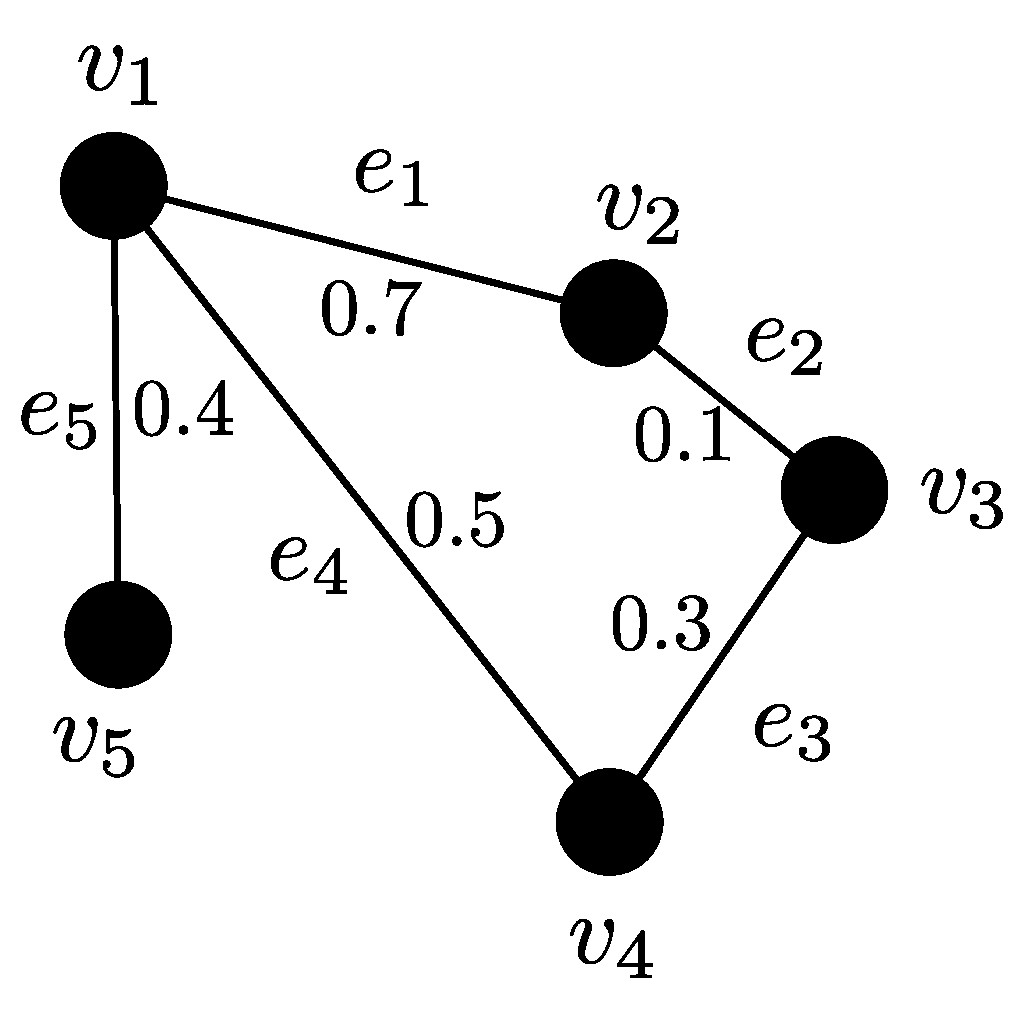
\includegraphics[width=0.5\textwidth]{example_graph.pdf}
%		\caption{Example graph.}
%		\label{fig:example_graph}
%	\end{center}
%\end{figure}
% ---
\begin{figure*}[!h]
	\centering	
	\hspace*{\fill}
	\begin{subfigure}[t]{0.32\textwidth}
		\subcaption{}
		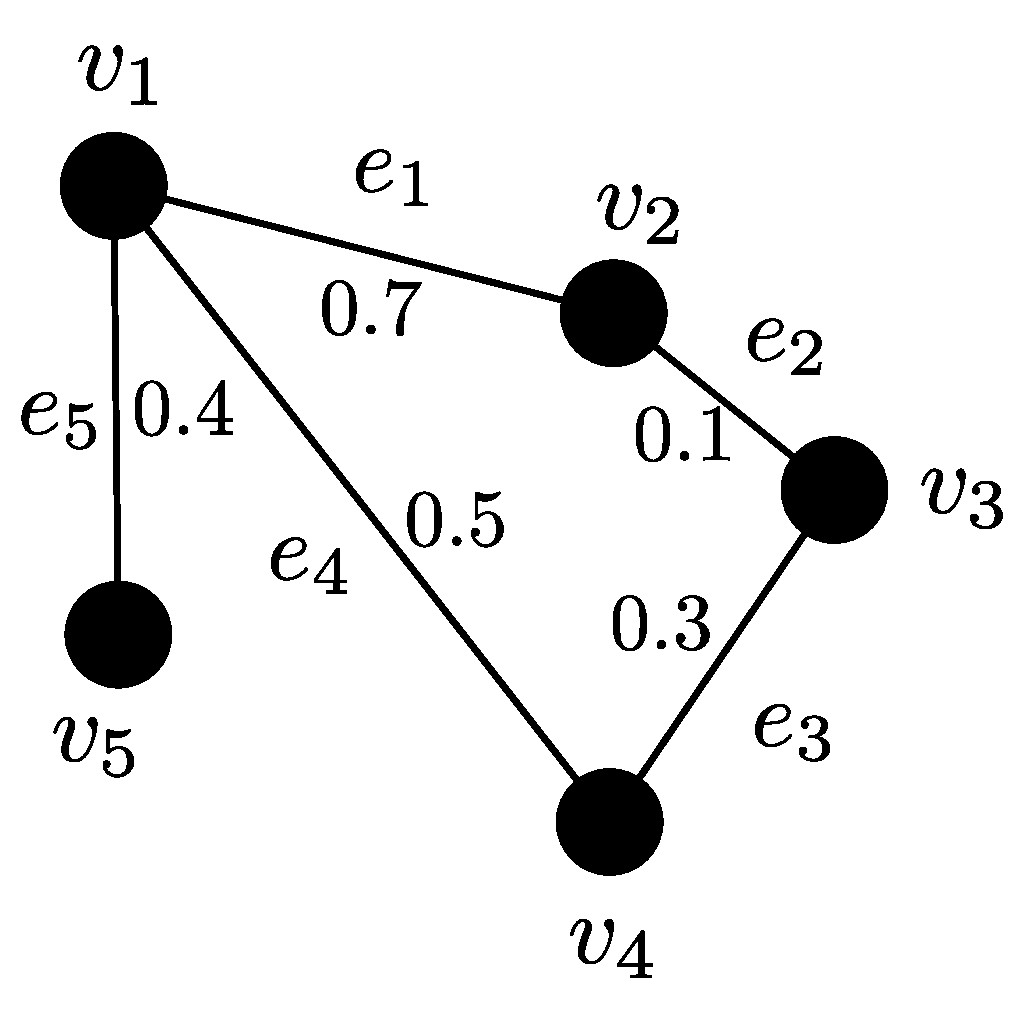
\includegraphics[width=\textwidth]{example_graph.pdf}
		\label{fig:example_graph}
	\end{subfigure}	
	\hfill
	\begin{subfigure}[t]{0.32\textwidth}
		\subcaption{}
		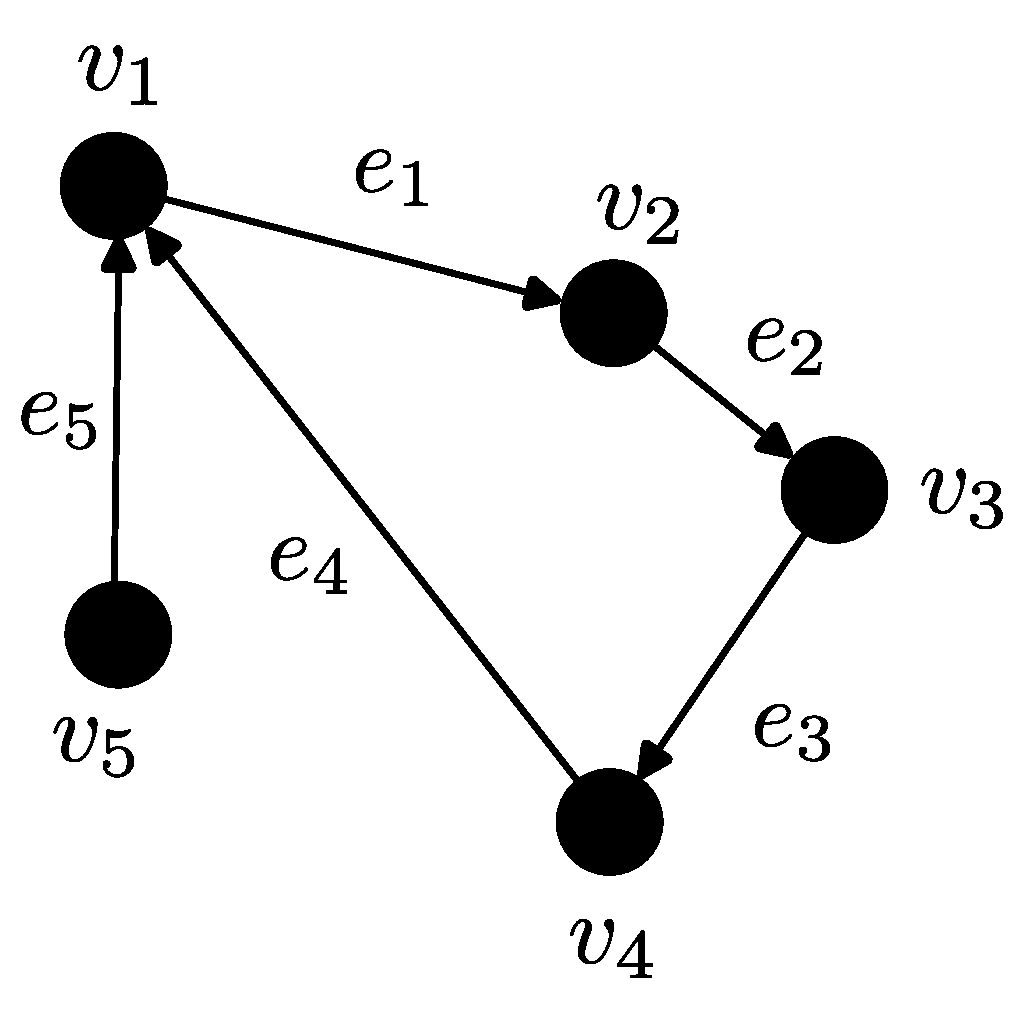
\includegraphics[width=\textwidth]{example_digraph.pdf}
		\label{fig:example_digraph}
	\end{subfigure}
	\hspace*{\fill}	
	\caption[] {\label{fig:graph_examples} \textbf{Two basic types of graphs}. (\subref{fig:example_graph}) An undirected and (\subref{fig:example_digraph}) a directed graph.}
\end{figure*}

%\begin{figure*}[!h]
%	\centering	
%	\hspace*{\fill}
%	\begin{subfigure}[t]{0.32\textwidth}
%		\subcaption{}
%		\includegraphics[width=\textwidth]{f6a_phantomx_hexapod.pdf}
%		\label{fig:phantomx_robot}
%	\end{subfigure}	
%	\hfill
%	\begin{subfigure}[t]{0.32\textwidth}
%		\subcaption{}
%		\includegraphics[width=\textwidth]{f6b_phantomx_pi_graph_kinematics.pdf}
%		\label{fig:phantomx_pigraph_kin_clusters}
%	\end{subfigure}
%	\hfill
%	\begin{subfigure}[t]{0.32\textwidth}
%		\subcaption{}
%		\includegraphics[width=\textwidth]{f6c_phantomx_morphology.pdf}
%		\label{fig:phantomx_morphology}
%	\end{subfigure}	
%	\hspace*{\fill}
%	\\
%	\hspace*{\fill}
%	\begin{subfigure}[t]{0.96\textwidth}
%		\subcaption{}
%		\includegraphics[width=\textwidth]{f6d_phantomx_morphology_errors_offline.pdf}
%		\label{fig:phantomx_morphology_errors_offline}
%	\end{subfigure}	
%	\hspace*{\fill}
%	\\
%	\hspace*{\fill}
%	\begin{subfigure}[t]{0.96\textwidth}
%		\subcaption{}
%		\includegraphics[width=\textwidth]{f6e_phantomx_morphology_errors_online.pdf} 		
%		\label{fig:phantomx_morphology_errors_online}
%	\end{subfigure}	
%	\hspace*{\fill}	
%	\caption[] {\label{fig:hexapod_simulated_results} \textbf{The hexapod robot}. (\subref{fig:phantomx_robot}) the PhantomX hexapod robot with its IMUs (red spheres), (\subref{fig:phantomx_pigraph_kin_clusters}) the kinematics graph $\mathcal{G}^{\mathcal{K}}_\pi$, (\subref{fig:phantomx_morphology}) the learned kinematic structure, errors in the estimated body structure via (\subref{fig:phantomx_morphology_errors_offline}) offline learning and (\subref{fig:phantomx_morphology_errors_online}) online learning (blue: difference rotation errors $\bar{\delta}~[\text{rad}]$, orange: sensor-to-sensor vector errors $\bar{\tilde{r}}~[\text{m}]$).}
%\end{figure*}
Two nodes $i$ and $j$ are said to be \emph{adjacent} if there is an edge $e$ connecting them. Similarly, the edge $e$ connecting the nodes is called \emph{incident} to $i$ and $j$. For example, the nodes $v_1$ and $v_4$ in Fig.~\ref{fig:example_graph} are adjacent to each other and the edge $e_4$ is incident to both nodes. The number of edges that are incident to a node is the \emph{degree} of the vertex. 

A \emph{path} represents a potential sequence of edges connecting any two given nodes. The number of edges determines the \emph{length} of the path. A graph is said to be \emph{connected} if there is at least one path between every pair of nodes; otherwise, it is labeled \emph{disconnected}. A \emph{cycle} constitutes a path comprising a minimum of three edges, where the initial and final vertices are identical, and no vertices are repeated in between. Lastly, a graph is \emph{complete} if there exists a path connecting every pair of nodes. Notice that the maximum number of edges in an undirected graph with $n$ nodes is $n(n-1)/2$

An \emph{undirected} graph lacks any specified direction assigned to its edges, meaning the connections between nodes are bidirectional. On the other hand, a \emph{directed} graph, commonly referred to as a \emph{digraph}, introduces directionality to its edges. In a directed graph, each edge has an explicit direction, indicating a one-way flow from one node to another. This directional information adds an extra layer of complexity to the relationships within the graph, as opposed to the bidirectional nature of edges in an undirected graph.

%A graph (or network) is a structure  that expresses the relationships between a set of vertices $ \mathcal{V}=\left\lbrace v_i\right\rbrace^m_{i=1}$ via a set of edges $ \mathcal{E}\subseteq \mathcal{V} \times \mathcal{V} $ with weights $ \bm{W}: \mathcal{V} \times \mathcal{V}\to \mathbb{R}_+$. Known as the weighted adjacency matrix, $ \bm{W} $ serves as the algebraic representation of $\mathcal{G}$.
A \emph{weighted} graph $ \mathcal{G}\big(\mathcal{V},\mathcal{E},\bm{W}\big) $ associates numerical value, a weight, to each edge. The weights with weights $ \bm{W}: \mathcal{V} \times \mathcal{V}\to \mathbb{R}_+$ express some quantitative measure such as distance, cost, time, or any other relevant metric depending on the context of the graph. Unlike an unweighted graph, where edges simply represent connections between nodes, a weighted graph provides additional information about the relationships between nodes. For a weighted graph, the \emph{strength} of a vertex corresponds to the sum of the edge weights associated with it.


\subsection{Algebraic representation of a graph}
A graph with $n$ vertices can be represented as a square $n\times n$ matrix $\bm{A}$. This algebraic representation is called the \emph{adjacency matrix} and depicts the graph's connectivity pattern; that is, the elements of the matrix indicate whether pairs of vertices $\left(i,j\right)$ are adjacent or not in the graph. Formally,
the elements of a \emph{binary} adjacency matrix $\bm{A}$ are determined as follows
% ---
\begin{equation}
	\left(\bm{A}\right)_{i,j} =
	\begin{cases}
		1 & \text{if and edge connects nodes $i$ and $j$}\\
		0 & \text{otherwise}.
	\end{cases}
\end{equation}
% --
By extension, a \emph{weighted} adjacency matrix $\bm{W}$ denotes a weighted connection for some of the $\left(i,j\right)$ entries, i.e $\left(\bm{W}\right)_{i,j} \in \mathbb{R}_+$. If the graph is undirected, the adjacency matrix is symmetric, which implies that $\bm{A}=\bm{A}^\intercal$ and $\bm{W}=\bm{W}^\intercal$respectively. Note, however, that for the case of digraphs, the adjacency matrix is not necessarily symmetric. To illustrate this, refer to the graph in Fig.~\ref{fig:example_graph}, the corresponding binary and weighted adjacency matrices are
% ---
\begin{equation*}
	\bm{A} = \begin{bmatrix}
		0 & 1 & 0 & 1 & 1\\
		1 & 0 & 1 & 0 & 0\\
		0 & 1 & 0 & 1 & 0\\
		1 & 0 & 1 & 0 & 0\\
		1 & 0 & 0 & 0 & 0\\
	\end{bmatrix}
\end{equation*} 
% ---
and
\begin{equation*}
	\bm{W} = \begin{bmatrix}
		0 & 0.7 & 0 & 0.5 & 0.4\\
		0.7 & 0 & 0.1 & 0 & 0\\
		0 & 0.1 & 0 & 0.3 & 0\\
		0.5 & 0 & 0.3 & 0 & 0\\
		0.4 & 0 & 0 & 0 & 0\\
	\end{bmatrix}.
\end{equation*} 
% ---
Similarly, for the digraph in Fig.~\ref{fig:example_digraph}, the adjacency matrix is
% ---
\begin{equation*}
	\bm{A}_D = \begin{bmatrix}
		0 & 1 & 0 & 0 & 0\\
		0 & 0 & 1 & 0 & 0\\
		0 & 0 & 0 & 1 & 0\\
		1 & 0 & 0 & 0 & 0\\
		1 & 0 & 0 & 0 & 0\\
	\end{bmatrix}.
\end{equation*} 
% ---
Notice that unless there are self loops in the graph, the main diagonal of an adjacency matrix contains only zero entries. Two other important matrices related to a graph $ \mathcal{G} $ are the degree matrix $ \bm{D}: (\bm{D}_{ii})=\sum_{j=1}^{m} w_{ij} $, a diagonal matrix whose entries are the sum of the rows of $ \bm{W} $, and the combinatorial graph Laplacian (CGL), defined as $ \bm{L}_\text{CGL} = \bm{D} - \bm{W} $ \cite{Mateos2019ConnectingdotsIdentifying}.

\subsubsection{The normalized adjacency matrix} 
The normalized adjacency matrix, defined as
% ---
\begin{equation}
	\mathbfcal{W} = \bm{D}^{-\frac{1}{2}} \bm{W} \bm{D}^{-\frac{1}{2}},
\end{equation}
% --- 
is particularly employed in spectral graph theory \cite{Spielman2012Spectralgraphtheory} and related analyses. Normalization helps account for variations in node degrees and provides a more balanced representation of the graph structure. One common application is in spectral clustering algorithms \cite{VonLuxburg2007tutorialspectralclusteringa}, where the normalized adjacency matrix is used to compute eigenvectors and eigenvalues, aiding in the identification of clusters or communities within a graph. %It also finds applications in various graph-based machine learning and data mining tasks.

\subsection{Subgraphs and spanning trees}
A \emph{subgraph} $\mathcal{G}_1$ is obtained by selecting a subset of the nodes of another graph $\mathcal{G}$ and a corresponding subset of the edges connecting those nodes. Formally, a graph $\mathcal{G}_1\left(\mathcal{V}_1, \mathcal{E}_1\right)$ is a subgraph of $\mathcal{G}$ if and only if $\mathcal{V}_1 \subseteq  \mathcal{V}$ and $\mathcal{E}_1 \subseteq \mathcal{E}$. This is written $\mathcal{G}_1 \subseteq \mathcal{G}$. One particular subgraph of interest in this work are spanning trees. First, a \emph{tree graph} is a graph that does not contain cycles. Such structure usually depicts a hierarchical arrangement. Consequently, a \emph{spanning tree} $\mathcal{G}_1$ of a graph $\mathcal{G}$ is a subgraph containing all the nodes in $\mathcal{G}$ and whose edges form a tree that defines paths that ensure that all the nodes remain connected. The edges of $\mathcal{G}_1$ are denoted as the branches of the tree. In general, a graph $\mathcal{G}_1$ is said to be a spanning subgraph of $\mathcal{G}$ if and only if $\mathcal{V}_1 = \mathcal{V}$ and $\mathcal{E}_1 \subseteq \mathcal{E}$. It is worth noting that every connected graph has a spanning tree and that there are $n^{n-2}$ distinct spanning trees with $n - 1$ edges on a connected graph with $n$ vertices \cite{West2001Introductiongraphtheory}. Examples of spanning trees are shown in Fig.~\ref{fig:tree_examples}.

\subsubsection{Minimum spanning tree and Kruskal's algorithm}
The minimum spanning tree of an undirected, connected, and weighted graph is the spanning tree whose edge weight sum is less than or equal to that of all other spanning trees \cite{Sefidgarminimumspanningtree}. Kruskal's algorithm \cite{Kershenbaum1972Computingminimumspanning} is the standard method to find th minimum spanning tree of a graph. In this work we use an equivalent concept, the \emph{maximum spanning tree} (MST), which corresponds to the spanning tree with maximum edge weight sum.
% ---
\begin{figure*}[!t]
	\centering	
	\hspace*{\fill}
	\begin{subfigure}[t]{0.32\textwidth}
		\subcaption{}
		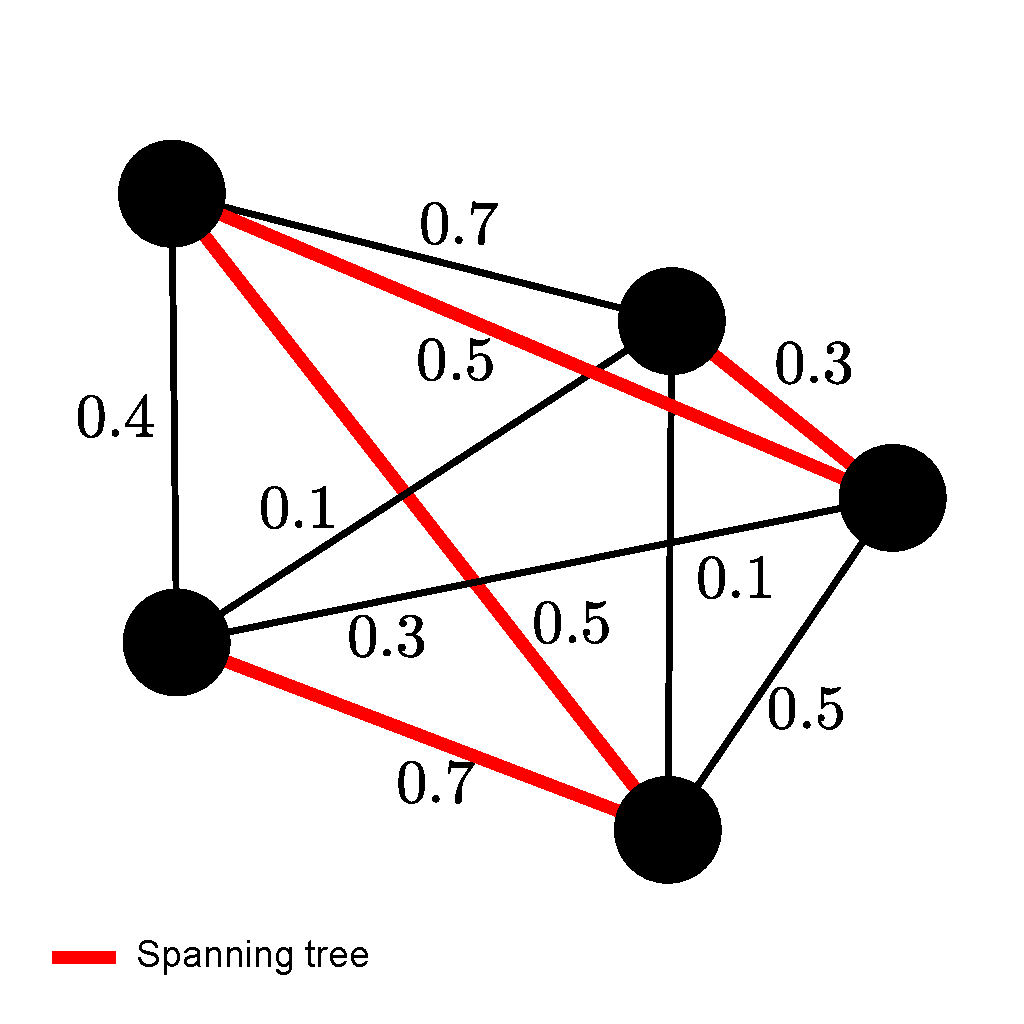
\includegraphics[width=\textwidth]{example_tree_1.pdf}
		\label{fig:example_tree_1}
	\end{subfigure}	
	\hfill
	\begin{subfigure}[t]{0.32\textwidth}
		\subcaption{}
		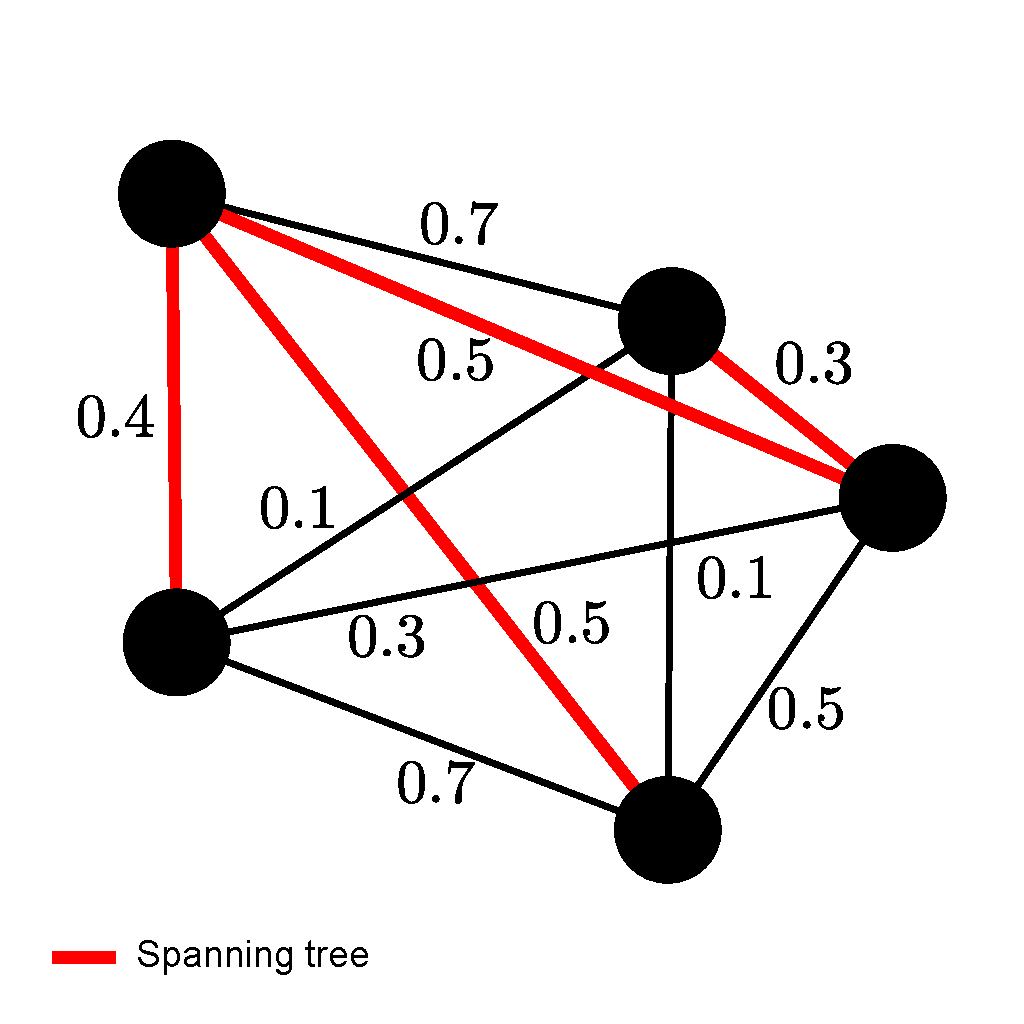
\includegraphics[width=\textwidth]{example_tree_2.pdf}
		\label{fig:example_tree_2}
	\end{subfigure}
	\hfill
	\begin{subfigure}[t]{0.32\textwidth}
		\subcaption{}
		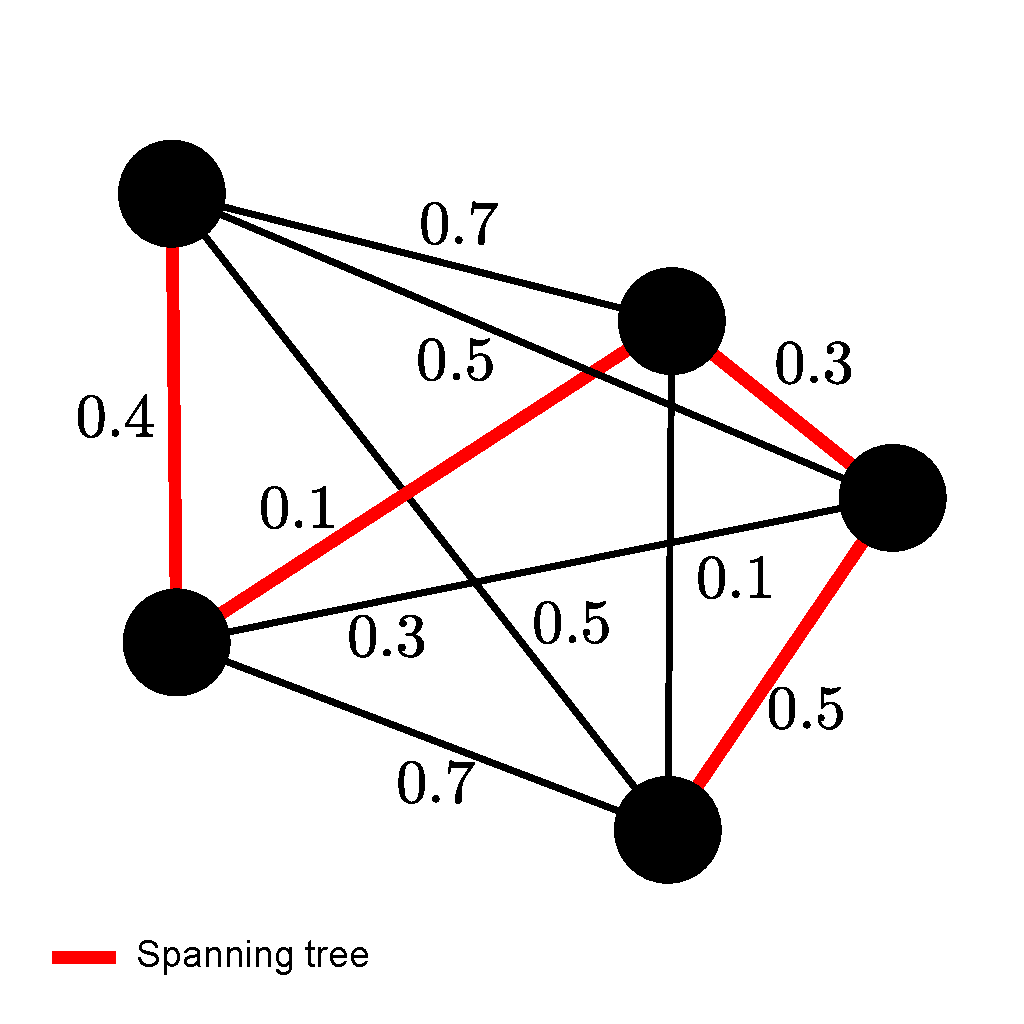
\includegraphics[width=\textwidth]{example_tree_3.pdf}
		\label{fig:example_tree_3}
	\end{subfigure}	
	\hspace*{\fill}	
	\caption[] {\label{fig:tree_examples} \textbf{Different spanning trees for the same graph}.}
\end{figure*}



\subsection{Metrics for graph comparison}
\TODO

% ===========================================================================================
%                                           |                                               |
% -------------------------------------- SECTION -------------------------------------------|
%                                           |                                               |
% ===========================================================================================
\section{Network topology inference}
The process of identifying and visually representing relationships among various elements within a system, based on the available measurements, is termed \emph{network topology inference} (NTI) \cite{Dong2019Learninggraphsdata}. Unveiling the structure of a network or graph through topology learning facilitates the analysis of interactions among entities. 

\subsection{Types connectivity}
%Finding and graphically representing the relationships among the different constituent elements of a system given the available measurements is known as \emph{network topology inference} (NTI) \cite{Dong2019Learninggraphsdata}. By learning the topology of a network/graph, it is possible to reveal a structure that aids in the analysis of the interaction among the entities. As discussed in \cite{Friston2011Functionaleffectiveconnectivity}, one method to represent interaction is via \emph{functional connectivity} (FC), which is an information-theoretic
%measure that characterizes dependencies based on the probability distributions of the observed signals (examples include correlations and mutual information). FC can be further subdivided into non-directed and directed, with the latter being related to statistical causation from the data \cite{Bastos2016tutorialreviewfunctional}. In contrast, \emph{effective connectivity} refers explicitly to the dynamic (state-dependent) influence that one element on the network has on another under a particular network model of causal dynamics; i.e, it refers to coupling or directed causal influence \cite{Park2013Structuralfunctionalbrain}. Exemplary works that use the concepts above can be found in biology\cite{Zhang2017Networkbasedmachine} and neuroscience \cite{Karwowski2019Applicationgraphtheory,Sporns2018Graphtheorymethods}.

\begin{figure*}[!h]
	\centering	
	\hspace*{\fill}
	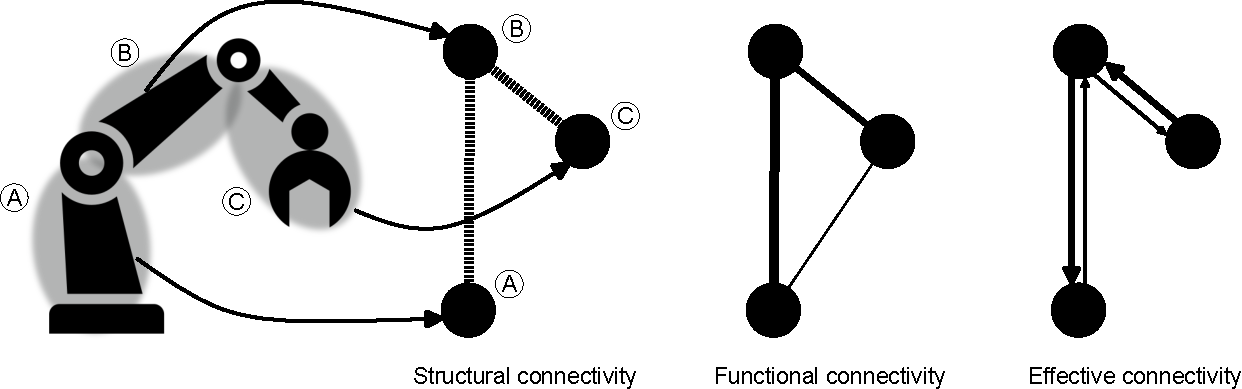
\includegraphics[width=0.9\textwidth]{types_of_connectivity.pdf}
	\hspace*{\fill}	
	\caption[] {\label{fig:types_of_connectivity}\textbf{Types of connectivity.} Every rigid body in the robot represents a node in the graphs.}
\end{figure*}

Often used in the field of neuroscience \cite{Karwowski2019Applicationgraphtheory}, three different types of connectivity are distinguished\cite{Park2013Structuralfunctionalbrain,FaskowitzEdgesbrainnetworks}:

\paragraph*{Structural Connectivity (SC).} Refers to the physical connections between different elements in a network. In the context of neuroscience, it typically involves the anatomical connections between brain regions. It is measured with techniques such as diffusion-weighted imaging (DWI) or diffusion tensor imaging (DTI) are commonly used to infer structural connectivity in the brain.

\paragraph*{Functional Connectivity (FC).} Refers to the statistical dependencies or temporal correlations between the activity of different elements in a network. As explained in \cite{Friston2011Functionaleffectiveconnectivity}, FC is an information-theoretic metric that characterizes dependencies using probability distributions of observed signals. It can be categorized into non-directed and directed forms, with the latter being associated with statistical causation derived from the data \cite{Bastos2016tutorialreviewfunctional}. %FC is often assessed through statistical methods applied to time-series data to identify patterns of correlated activity between different brain regions.

\paragraph*{Effective Connectivity (EC).} Specifically addresses the dynamic, state-dependent influence that one network element has on another within a particular causal dynamics model. Essentially, effective connectivity denotes coupling or directed causal influence \cite{Park2013Structuralfunctionalbrain}. Exemplary applications of these concepts can be observed in the fields of biology \cite{Zhang2017Networkbasedmachine} and neuroscience \cite{Karwowski2019Applicationgraphtheory,Sporns2018Graphtheorymethods}.

To understand the intricate relationships among the three types of connectivity refer to Fig.~\ref{fig:types_of_connectivity}. The figure depicts a simple robot arm as an example. The nodes represent the three links that compose the robot. Regarding SC and FC, a nuanced connection exists, albeit not strictly one-to-one. For example, the SC reflect the physical composition of the body, three bodies connected by two joints (the edges in the SC graph). Sensory signals coming from these bodies might lead to potential functional interactions of varied degree (the edges in the FC graph) that have a foundation on the bodily structure of the robot; yet, it does not ensure their occurrence. Actually, functional relationships can appear even in the absence of direct structural connections, not the light edge between nodes $A$ and $C$ in the FC graph. Moving to EC and FC, the former extends the latter by seeking to model the direction and strength of influence between different elements. While FC identifies statistical associations, EC strives to unveil the underlying causal relationships, the directed edges in the EC graph. In summary, these three connectivity types are interrelated components in the complex landscape of NTI. Structural connections provide the anatomical substrate, functional connections depict statistical dependencies, and effective connections aspire to model causal relationships within the network.


%\redtext{The relationships between SC, FC, and EC in NTI are intricate and multifaceted. Regarding structural and functional connectivity, a nuanced connection exists, albeit not strictly one-to-one. Structural connectivity establishes the anatomical foundation for potential functional interactions, but it doesn't ensure their occurrence. Notably, functional correlations can manifest even in the absence of direct structural connections. Moving to effective connectivity and functional connectivity, the former extends the latter by seeking to model the direction and strength of influence between different elements. While functional connectivity identifies statistical associations, effective connectivity delves deeper, striving to unveil the underlying causal relationships. In summary, these connectivity types are interrelated components in the complex landscape of network topology inference. Structural connections provide the anatomical substrate, functional connections depict statistical dependencies, and effective connections aspire to model causal relationships within the network.} %While these concepts are often explored within the realm of neuroscience, their principles are versatile and applicable to understanding other intricate systems beyond the brain.
%**Relationships:**
%- **Structural and Functional Connectivity:** There is a relationship between structural and functional connectivity, but it's not one-to-one. Structural connectivity provides the anatomical substrate for potential functional interactions, but structural connections do not guarantee functional interactions, and functional correlations can occur in the absence of direct structural connections.
%
%- **Effective Connectivity and Functional Connectivity:** Effective connectivity builds upon functional connectivity by attempting to model the direction and strength of the influence between different elements. While functional connectivity identifies statistical associations, effective connectivity aims to infer the underlying causal relationships.
%
%In summary, structural, functional, and effective connectivity are interrelated aspects of network topology inference, with structural connections providing the anatomical substrate, functional connections representing statistical dependencies, and effective connections aiming to model causal relationships within the network. Techniques from neuroscience are often applied to study these aspects in the context of brain networks, but similar principles can be extended to other complex systems.

\subsection{Inferring the connectivity}
In NTI the elements $\mathcal{V}$ of a graph $\mathcal{G}$ are known but its connectivity (i.e. how these elements relate to each other) is unknown. Then, the graph topology inference problem consists in finding the edges $\mathcal{E}$ that best explain the relationships among the nodes $\mathcal{V}$ given some prior knowledge, such as  data distribution, the location of the sensors, the physical relationships between the signals, or the data similarity \cite{Dong2019Learninggraphsdata,Stankovic2019Introductiongraphsignal}. 

With \textbf{mutual information} \cite{Villaverde2014MIDERnetworkinference}

With \textbf{GSP} \cite{Dong2019Learninggraphsdata}. We consider a method \cite{Kalofolias2016Howlearngraph} which learns a relational matrix $ \bm{W}_{GSP} $ without prior structural information considering the signals in $\bm{x}(t) $ as graph signals\cite{Dong2019Learninggraphsdata}. $ \bm{W}_{GSP} $ is derived under the assumption that the signals on the graph change smoothly between connected nodes. Likewise, the Graph Signal Processing Toolbox (GSPBOX) from \cite{Perraudin2014GSPBOXtoolboxsignal} was used to compute $ \bm{W}_{GSP} $ using $\alpha = 0.6$, $\beta  = 1$ (parameters that control the edge weight magnitude and the sparsity of $ \bm{W}_{GSP} $, respectively) and normalizing the required pairwise distance matrix $\bm{Z}$ between $[0,1]$.

With \textbf{correlation}. The first technique \cite{Olsson2006unknownsensorsactuators} upgrades standard correlation-based NTI by searching for an inverse covariance matrix with Laplacian (to find valid adjacency matrices $ \bm{W}_{cor} $) and structural constraints (requiring a sparse matrix to reduce the graph edge density). We used the Graph Laplacian Learning (GLL) package \cite{Egilmez2021GraphLaplacianLearning} to calculate $ \bm{W}_{cor} $, with regularization parameter $\gamma = 0.07$ and using a matrix $\bm{W}_0$ as connectivity prior with zero diagonal elements and ones elsewhere (denoting lack of structural knowledge).










\hrule

\subsubsection{Challenges in NTI}
NTI brings with it challenges such as noisy measurements, lack of ground truth, large parameter spaces, and varying model complexity \cite{Brugere2018Networkstructureinference}. Moreover, inferring graph topology only from data is an ill-posed problem, having statistical models (e.g. correlation, entropy, mutual information) and physically motivated models (e.g. network diffusion) as general approaches \cite{Dong2019Learninggraphsdata}. %Statistics-based models entail methods based on correlation, probabilistic graphical models, as well as methods based on concepts such as entropy, mutual information and transfer entropy. Physically motivated models consider the data to be generated by an underlying physical phenomenon on the graph, such as network diffusion. 
Finally, the recently introduced paradigm of Graph Signal Processing (GSP) \cite{Stankovic2019Introductiongraphsignal} considers samples from the signals at a given time as \emph{graph signals}, whose properties are a consequence of the underlying graph. %Excellent works that discuss NTI via GSP methods can be found in \cite{Dong2019Learninggraphsdata,Mateos2019ConnectingdotsIdentifying,Stankovic2019Introductiongraphsignal}.


\subsection{Detecting linear dependencies with covariance}
\subsection{Graph signal processing}
The fairly recent field of Graph Signal Processing (GSP) \cite{Mateos2019ConnectingdotsIdentifying}

\redtext{Under the assumption that the signals are related to the topology of the graph where they are supported, the goal of GSP is to develop algorithms that fruitfully leverage this relational structure and can make inferences about these
	relationships even when they are only partially observed.}

A network may represent a conceptual model of pairwise relationships

A fundamental question in GSP is how to use the graph signals to infer the underlying structure of the network.

\subsection{Based on statistic measures}

% ===========================================================================================
%                                           |                                               |
% -------------------------------------- SECTION -------------------------------------------|
%                                           |                                               |
% ===========================================================================================
\section{Information theory}
As discussed in \cite{Cover1999Elementsinformationtheory} information is$\ldots$
¸\subsection{The meaning information}
\subsection{Entropy of random variables}
\subsection{Mutual Information: The correlation of the 21st century }
\subsection*{Mutual information}
The mutual information between two random variables is a symmetric measure of information computed as:
% ---
\begin{equation}\label{eq:mutual_information}
	I\left(X;Y\right) =I\left(Y;X\right) = H(X) + H(Y) - H(X,Y)
\end{equation}
% ---
with the Shannon's entropy of a variable $X$ defined by 
% ---
\begin{equation}\label{eq:entropy}
	H(X) = -\sum_{i=1}^{n}p(x_i)\text{log}_2\left(p\left(x_i\right)\right)
\end{equation}
% ---
and the joint entropy between $ X $ and $ Y $ expressed as
% ---
\begin{equation}\label{eq:joint_entropy}
	H(X,Y) = -\sum_{i=1}^{n}\sum_{j=1}^{n} p(x_i,y_j)\text{log}_2\big(p\left(x_i,y_j\right)\big).
\end{equation}
% ---

%As mentioned in the main text, the MI is used to create the relational matrix $\hat{\bm{W}}_{MI}$. In practice, the computation of $(\hat{\bm{W}}_{MI})_{i,j}$ involves selecting a pair $\left({x}_i(t),{x}_j(t)\right)$ of time series from the data matrix $\bm{X}$, centering their samples (to zero mean and unit standard deviation) and using either binning, kernel, or nearest neighbor methods \cite{WaltersWilliams2009Estimationmutualinformation} to compute their mutual information. Yet, such a process can be memory- and computation-demanding when the length $n$ of each of the time series is large or when streaming signals are considered. Therefore, to enable the online computation of the $m\left(m-1\right)/2$ pairwise MI values, every $N_{\mathbfcal{X}}$ points, we extract a mini-batch $\mathbfcal{X}$ from the replay buffer $\mathbfcal{B}$ and compute its corresponding MI matrix $\bm{W}^\mathbfcal{X}_{MI}$. Then, the overall MI matrix estimate $\hat{\bm{W}}_{MI}$ for the time series is the cumulative average over the previously computed matrices $\bm{W}^\mathbfcal{X}_{MI}$. To monitor its convergence, we observe the total information content in the matrix, defined as
%% ---
%\begin{equation}\label{eq:total_information}
%	T_{MI} =  \frac{1}{2}\text{tr}\left(\hat{\bm{D}}_{MI}\right),
%\end{equation}
%% ---	
%where $\hat{\bm{D}}_{MI}$ is the associated degree matrix. After the change in $T_{MI}$ falls below a threshold value $\epsilon$, namely 
%$\Delta T_{MI}<\epsilon$, $\hat{\bm{W}}_{MI}$ exhibits minimal changes in its structure. In Sec.~\nameref{sec:topology_convergence}, we provide examples of the convergence of this term for the robot manipulator, hexapod, and humanoid cases.
%
%In this work, for the computation of $\hat{\bm{W}}_{MI}  $ either offline from $\bm{X}$ or incrementally from the mini-batch matrices $\bm{W}^\mathcal{X}_{MI}$, we use the Java Information Dynamics Toolbox (JIDT) \cite{Lizier2014JIDTinformationtheoretic} and choose a kernel method to compute the MI from the signals $ \bm{x}(t) $ with a kernel width of $k = 0.8$. We alternatively used the Python machine learning library scikit-learn\cite{Pedregosa2011ScikitlearnMachine} and the open-source MATLAB package Mutual Information Computation \cite{PengMutualInformationcomputation} for comparison.

\subsubsection{Unexplored alternatives}
The transfer entropy \cite{Bossomaier2016introductiontransferentropy} is

% ===========================================================================================
%                                           |                                               |
% -------------------------------------- SECTION -------------------------------------------|
%                                           |                                               |
% ===========================================================================================
\section{Differential geometry}
\subsection{Fundamentals of differential geometry}
\subsection{Manifolds and the tangent space}
\subsection{Riemannian geometry and the metric}
\subsection{Applications in robotics}

\say{The Symmetric Positive Definite (SPD) manifold is one specific type of Riemannian manifold. It is a smooth manifold where the tangent space is endowed with a Riemannian metric [2]. The Riemannian metric allows us to define various geometric notions such as the geodesic distance.}

%% ===========================================================================================
%%                                           |                                               |
%% -------------------------------------- SECTION -------------------------------------------|
%%                                           |                                               |
%% ===========================================================================================
%\section{Model learning in robotics}
%Existing learning frameworks often focus on developing forward and inverse models using either a global or local approach to capture input-output relationships \cite{NguyenTuong2011Modellearningrobot}.
%
%Global methods risk overfitting and computational overload, while local methods suffer from limited generalization and hyperparameter sensitivity \cite{Thrun2002Probabilisticrobotics,Goodfellow2016DeepLearning}. Despite advancements in computational power and data availability, deep learning faces challenges due to the neglect of prior principled knowledge, making it difficult to determine dedicated neural network architectures \cite{Baker2017Designingneuralnetwork,Elsken2019Neuralarchitecturesearch}. 
%
%\subsection{End-to-end learning}
%
%\subsubsection{Classical neural networks model learning}
%Model-learning problems using neural networks (NN) mainly involves:
%\begin{enumerate}
%	\item Input/output data collection: assumed to be available
%	\item Architecture design: usually found by trial and error
%	\item Parameter optimization/learning: via well understood schemes, e.g., backpropagation and variants
%\end{enumerate}
%Designing NN for a particular problem requires experts to determine the best topology, i.e. the number of nodes and layers, connectivity, and activation functions \cite{Matteucci2006ELeaRNTEvolutionarylearning}. Furthermore, generalization is difficult as the architecture needs to balance achieving accuracy while avoiding overfitting \cite{Rocha2005Simultaneousevolutionneural,He2015Topologicaloptimisationartificial,Matteucci2006ELeaRNTEvolutionarylearning,Kwok1995Constructivefeedforwardneural,Lawrence1998Whatsizeneural,Talebi2010NeuralNetworkBased}. Therefore, if a NN is used without any model information, large amounts of training data are required to generalize to unknown data \cite{Urolagin2012Generalizationcapabilityartificial}.
%
%\subsubsection{Topology learning related works}
%Finding NN topologies is an important and challenging step \cite{Tirumala2016Evolvingdeepneural,Rocha2005Simultaneousevolutionneural,Baker2017Designingneuralnetwork}. Normally, function approximation via NN uses empirical topologies that rely on numerous parameters and do not lend themselves to interpretation. Such models provide no insight into the actual relation between the system variables. Recent works have aimed to find optimal topologies automatically. For example, evolutionary methods have been utilized to optimize the topology of Feed Forward NN (FFNN) \cite{Rocha2005Simultaneousevolutionneural,Matteucci2006ELeaRNTEvolutionarylearning} as well as  deep NN \cite{Tirumala2016Evolvingdeepneural}, by adding/deleting connections and weights. Constructive methods \cite{Kwok1995Constructivefeedforwardneural} and pruning methods \cite{Srinivas2016LearningNeuralNetwork} have also been applied to FFNN. Another method used for FFNN represents the network as a graph and reduces its degrees-of-freedom (DoF) \cite{He2015Topologicaloptimisationartificial}. Furthermore, reinforcement learning (through Q-learning) and topology learning (using variance analysis) have also been implemented to generate architectures \cite{Baker2017Designingneuralnetwork,Castillo2007Functionalnetworktopology}. Noticeably, for learning complex dynamical systems, such as articulated robot structures, results have been limited in accuracy and generalization capabilities \cite{NguyenTuong2011Modellearningrobot,NguyenTuong2008Learninginversedynamics,NguyenTuong2010Usingmodelknowledge}. 
%
%\subsubsection{Robot inverse dynamics estimation via classical NN}\label{sec:classic_inv_dyn}
%NN have been applied in numerous variants to model robot inverse dynamics. In \cite{Atencia2015Hopfieldnetworksoptimization}, Hopfield NN were applied to identify the inertial parameters. Likewise, in \cite{Zhu2014Inertiaparameteridentification} a FFNN that used the regressor matrix as training samples was applied. Extreme Learning Machines were utilized in \cite{Bargsten2016ExperimentalRobotInverse} with the same purpose. More recently a two-hidden-layers network with rectified linear activation units (ReLU) was used in \cite{Christiano2016TransferSimulationReal}. Similarly, recurrent NN have been used to account for the sequential nature of the data. In \cite{Yan1997Robotlearningcontrol}, a recurrent NN in the hidden layer of an otherwise conventional three-layer FFNN was proposed. Additionally, self-organizing-networks, in conjunction with echo state networks, were used in \cite{Polydoros2015Realtimedeep} via a real-time deep learning algorithm.
%% ===========================================================================================
%%                                           |                                               |
%% -------------------------------------- SECTION -------------------------------------------|
%%                                           |                                               |
%% ===========================================================================================
%\section{Data-driven learning with structure information}
%In lieu of the challenges faced by deep learning to capture the intricacies of complex systems from scratch,  
%Issues such as low sample efficiency, extended training times, and limited generalization highlight the necessity of balancing data-driven and principle-driven approaches \cite{Pierson2017Deeplearningrobotics,Suenderhauf2018limitspotentialsdeep}. Recently, there has been a growing acknowledgment of the importance of integrating structure into the learning of physical systems \cite{Geist2021Structuredlearningrigid,Lutter2023Combiningphysicsdeep}.
%
%% ===========================================================================================
%%                                           |                                               |
%% -------------------------------------- SECTION -------------------------------------------|
%%                                           |                                               |
%% ===========================================================================================
%\section{Model learning and the body schema}
%
%
%
%
%Building on the significance of structure in model learning for robotics, this dissertation addresses the inference of essential morphological properties in tree-like floating base structures, mimicking the development of a body schema. Efforts in cognitive robotics stress the pivotal role of internal body models in enhancing spatial awareness, motor control, and adaptability \cite{Nguyen2021Sensorimotorrepresentationlearning,Hoffmann2010Bodyschemarobotics}. However, consensus is lacking on what constitutes a robot's body schema. Some approaches focus solely on learning the kinematic structure, relying predominantly on off-body vision \cite{Hersch2008Onlinelearningbody,MartinezCantin2010Bodyschemaacquisition,Hart2011roboticmodelecological,Lipson2019Taskagnosticself,Chen2022Fullybodyvisual,Sturm2009Bodyschemalearning}. Others explore sensorimotor associations between proprioceptive, tactile, and visual modalities \cite{Fuke2007BodyImageConstructed,Malinovska2022connectionistmodelassociating,Nguyen2019Reachingdevelopmentvisuo,Pugach2019BrainInspiredCoding,Lanillos2016Yieldingselfperception}, but they provide limited insights into the robot's physical structure.
%
%Model-based robotics offers reliable methods for identifying physical attributes of robots based on known mechanical topologies. Conventional calibration routines \cite{Hollerbach1996CalibrationIndexTaxonomy} and offline system identification methods \cite{Swevers2007Dynamicmodelidentification,LeboutetInertialParameterIdentification} are effective for known kinematic structures in controlled environments. However, these methods face challenges when applied to floating base robots without standardized identification procedures \cite{Ayusawa2014Identifiabilityidentificationinertial,Lee2022OptimizedSystemIdentification}. Importantly, these conventional methods were not initially designed for integration into online learning frameworks. While model-based robotics addresses kinematic calibration and forward/inverse kinematics, it provides limited insights into the comprehensive understanding of joint and link arrangement, known as mechanical topology. In cognitive robotics, only a few studies have approached this problem for self-modeling and monitoring, relying on exteroceptive vision \cite{Bongard2006Automatedsynthesisbody,Bongard2006Resilientmachinescontinuous}. Regardless of the approach taken---black-box machine learning, cognitive methods, or model-based robotics---reliance on external measurement devices persists, overlooking embodied sensing modalities.
%
%In summary, current robotics research reveals gaps in understanding and methods for refining body models. A comprehensive interpretation of the robot body schema and the determination of essential features are crucial. Identifying the fundamental set of necessary signals, both proprioceptive and embodied exteroceptive, is paramount. Integrating advanced machine learning with prior information and first-order principles shows promise for enhanced body models, addressing data requirements and generalization issues. However, the lack of synergy between modeling and learning approaches, along with the absence of a unified scheme for relevant learning stages, represents notable gaps requiring attention to advance robotics into more sophisticated and adaptable embodied systems.
%
%\section{Model learning in robotics}
%\subsection{Classical and recent works in system identification}
%\subsection{Local and global models linear models}
%\subsection{End-to-end learning (black box models)}
%\section{Data-driven learning with structure information}
%\section{Model learning and the body schema}
%\subsection{Internal representations}
%\subsection{Sensorimotor maps}


\chapter{Methods: How to learn the robotic body schema}
We envision learning the robotic body schema as a series of learning stages that the robot must go through to discover core features of its body morphology. These features are part of the set 
% ---
\begin{equation}
	\mathcal{S} = \left\lbrace N, \mathcal{G}, \bm{A}, \bm{\lambda}, \bm{\theta} \right \rbrace
	\label{eq:self_elements},
\end{equation}
% ---
whose elements are the number of bodies $N$ in the kinematic chain, the graph $\mathcal{G}$ that describes the sensorimotor interactions that result from the robot's embodiment, the adjacency matrix $\bm{A}$ that captures the topology ---mechanical arrangement of the bodies and joints---, its kinematic description (basic geometry) $\bm{\lambda}$, and the inertial parameters of the links $\bm{\theta}$. Thus, a robot capable of acquiring knowledge of the elements of $\mathcal{S}$ is an agent that builds an understanding of its physical self. An overview of this process is depicted in Fig.~S1.

\chapter{Results}

\chapter{Discussion}
The results and approach presented in this work bear resemblance to the work by Sturm \cite{Sturm2009Bodyschemalearning}, Hersch\cite{Hersch2008Onlinelearningbody}, Bongard \cite{Bongard2006Resilientmachinescontinuous}, and Lipson \cite{Chen2022Fullybodyvisual}
%\chapter{Conclusion}
%
%\chapter{Test Chapter}
%%This chapter introduces the theoretical foundations on which the proposed learning architecture is built.
The fundamental element of the framework is the tactile skill formalism described in Sec.~\ref{ch:foundations:representation} consisting of the tactile platform, tactile controller, tactile policy, and a performance evaluator.
As a complementary component, a formal process definition is provided that describes industrial processes in terms of manipulation steps and boundary conditions such as error and success states.
In order to connect these two elements, a taxonomy is devised with a hierarchical structure that organizes tactile policies according to process properties.
Based on the tactile skill, process definition, and taxonomy, a synthesis procedure is presented that automatically selects a tactile policy that is suited to solve a given input process.
In Sec.~\ref{ch:foundations:planning} an assembly planner is introduced that makes direct use of the tactile skill concept and extends it to skill sequences. The planner solves the allocation problem for a team of humans and robots for a given assembly problem.
Finally, in Sec.~\ref{ch:foundations:learning} the basis for the learning architecture introduced in Ch.~\ref{ch:architecture} is introduced.
It presents a number of state-of-the-art learning algorithms that are used throughout this thesis as well as useful performance metrics to realize the performance evaluator.
Finally, a robot motor memory effect is described that was discovered in an earlier experiment. The effect forms the basis for the transfer learning experiments described in Ch.~\ref{ch:experiments}.
This chapter was written based on \cite{Johannsmeier.2017,Johannsmeier.2019,Johannsmeier.2023,Johannsmeier.2023b}.
%\section{Taxonomy Verification}\label{ch:experiments:taxonomy}
%In this final section the possible contribution of this thesis to future industrial applications as well as important new research directions are elaborated.

\section{Applications}
\input{chapter/outlook/applications}

\section{Further Research}
\input{chapter/outlook/research}
%\section{Tactile Skill Learning}\label{ch:experiments:learning}
%In this final section the possible contribution of this thesis to future industrial applications as well as important new research directions are elaborated.

\section{Applications}
\input{chapter/outlook/applications}

\section{Further Research}
\input{chapter/outlook/research}
%\section{Performance Comparison: Robot vs. Human}\label{ch:experiments:comparison}
%In this final section the possible contribution of this thesis to future industrial applications as well as important new research directions are elaborated.

\section{Applications}
\input{chapter/outlook/applications}

\section{Further Research}
\input{chapter/outlook/research}
%\section{Collaborative Assembly Planning}\label{ch:experiments:planning}
%In this final section the possible contribution of this thesis to future industrial applications as well as important new research directions are elaborated.

\section{Applications}
\input{chapter/outlook/applications}

\section{Further Research}
\input{chapter/outlook/research}
%\section{Conclusion}\label{ch:experiments:conclusion}
%This chapter describes the extensive experimental work done in this thesis.
Specifically, the taxonomy of manipulation skills is verified with a large number of challenging skills that exhibit high robustness and performance.
This shows that the approach is applicable to a wide range of relevant processes.
The learning architecture is experimentally validated with a number of different learning algorithms and a comparison with state-of-the-art deep learning methods.
The results aid in selecting compatible learning algorithms and show superior results when compared to the state-of-the-art.
Furthermore, a large experimental campaign is described that investigates the architecture’s transfer learning capabilities.
It demonstrates accelerated learning when reusing knowledge to learn new skills and provides insights into the transfer mechanism such as dependency on geometry and asymmetric transferability.
The learning performance as well as achieved manipulation performance were directly compared to human manipulation capabilities and skill programming. The results show that for some skills human performance can already be achieved, while also pointing out the specific gaps that still need to be closed.
Finally, a collaborative assembly problem is solved by an automatic planning system and a human-robot team demonstrating how existing skills can be used automatically to solve even complex tasks.


\section{Introduction}
\subsection{Contributions}
In this paper we cast robot system identification into an incremental learning problem integrating machine learning methods and first-order principles from mechanics and differential geometry. Moreover, we enforce physical conformity of the inertial properties at all times by seamlessly moving on the Riemannian manifold of symmetric positive definite (SPD) matrices, where the inertial parameters of a rigid body are known to reside. We implement a Riemannian gradient descent algorithm with adaptive learning rate and extend it with an experience replay buffer to accelerate convergence and cope with sensor noise. Unlike other approaches, we do not depend on informed initial values. Additionally, we analyze different force/torque measurement setups and evaluate their influence on the learning process. Finally, we implement the method on a real robot and investigate the quality of the inverse dynamics torques generated by the learned parameters and assess the modeling error via a momentum observer.


% ===================================================================================================
%                                                 |                                                 |
%                                                 |                                                 |
% -------------------------------------------- SECTION ---------------------------------------------|
%                                                 |                                                 |
%                                                 |                                                 |
% ===================================================================================================
\section{Literature review}\label{sec:literature_review}


% SUBSECTION ========================================================================================
\subsection{Related works}

\subsubsection{Classical neural networks model learning}
%Conventional neural networks (NN) are often applied to model-learning problems as depicted in Figure~\ref{fig:NN_ID}. The process involves, mainly, the following steps:
Model-learning problems using typical neural networks (NN) involves, mainly, the following steps:
\begin{enumerate}
	\item Input/output data collection: assumed to be available
	\item Architecture design: usually found by trial and error
	\item Parameter optimization/learning: via well understood schemes, e.g., backpropagation and variants
\end{enumerate}
Overall, NN design involves many meta parameters, i.e. number of nodes, numbers of layers, connectivity, activation functions; requiring experts to determine the best topology for a particular problem \cite{Matteucci2006ELeaRNTEvolutionarylearning}. Furthermore, it is difficult to achieve an acceptable level of generalization \cite{Rocha2005Simultaneousevolutionneural}\cite{He2015Topologicaloptimisationartificial}\cite{Matteucci2006ELeaRNTEvolutionarylearning}\cite{Kwok1995Constructivefeedforwardneural}\cite{Lawrence1998Whatsizeneural}\cite{Talebi2010NeuralNetworkBased} as the architecture needs to be balanced to obtain accurate results without overfitting, which may lead to poor generalization, \cite{He2015Topologicaloptimisationartificial}\cite{Muzhou2013NewConstructiveMethod}\cite{Talebi2010NeuralNetworkBased}. Therefore, if a non-parametric model, such as a NN, is used without any model information, large amounts of data are required to generalize to unknown data \cite{Urolagin2012Generalizationcapabilityartificial}.
%\begin{figure}
%    \centering
%    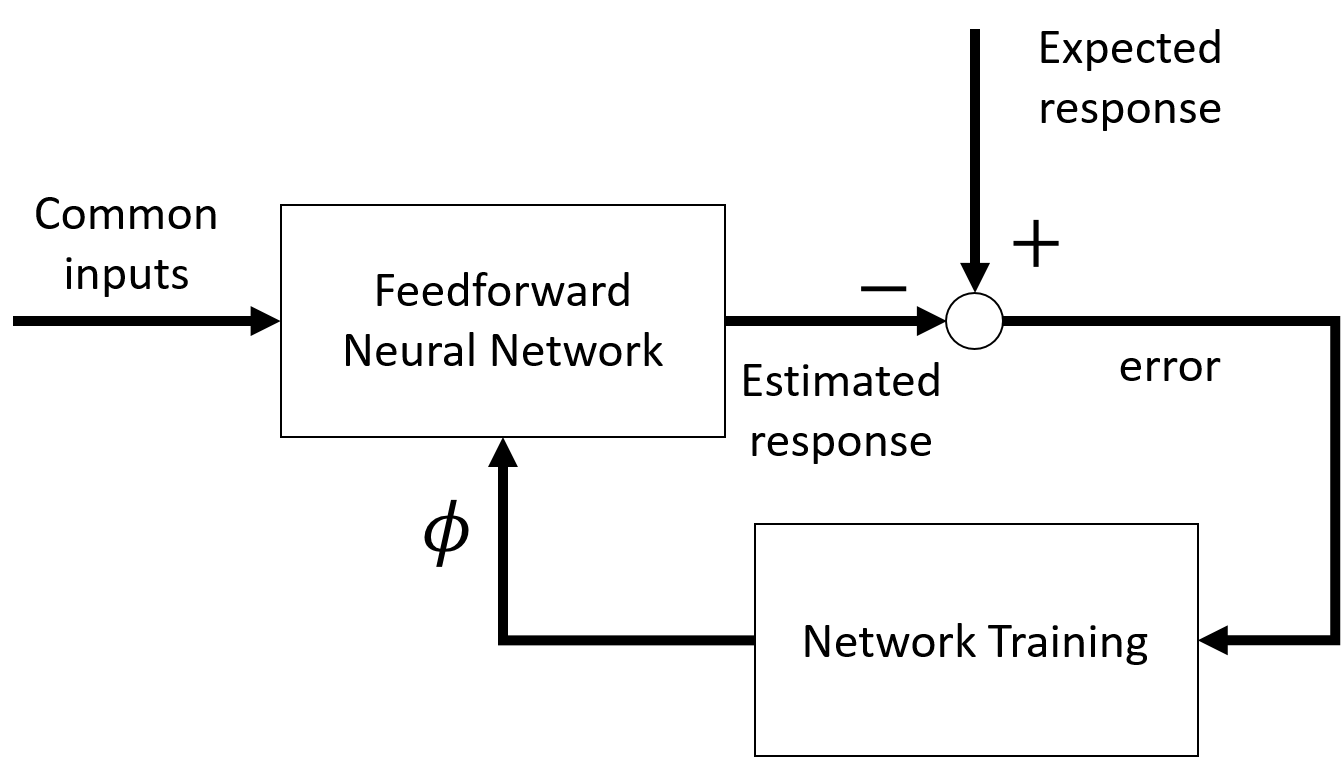
\includegraphics[width=0.3\textwidth]{fig/generalNN_ID}
%    \caption{General model learning using neural networks.}
%    \label{fig:NN_ID}
%\end{figure}

\subsubsection{Topology learning related works}
Finding NN topologies is an important and challenging step \cite{Miikkulainen2017EvolvingDeepNeural}\cite{Rocha2005Simultaneousevolutionneural}\cite{Baker2017Designingneuralnetwork}. Function approximation using NN uses subjective or empirical topologies that are, however, not suitable for interpretation and rely on numerous parameters. As a result, such models are not able to give insight into the actual relation between system variables. 

%As defined in \cite{Matteucci2006}: \textit{"The problem of finding an optimal topology can be thought of as a search problem, where the search space is the space of all possible network topologies, and where the goal is to minimize an error function while preserving generalization capabilities"}. 

Recent works have aimed to find optimal topologies automatically. Evolutionary methods are commonly utilized to optimize the topology and the weights of NN by adding or deleting connections and weights, as shown in \cite{Rocha2005Simultaneousevolutionneural} and \cite{Matteucci2006ELeaRNTEvolutionarylearning} for Feed Forward Neural Networks (FFNN) or \cite{Miikkulainen2017EvolvingDeepNeural} for deep NN. Results tend to show satisfactory generalization capabilities, comparable to human designs. Another method used for FFNN represents the network as a graph and reduces its degrees-of-freedom (DoF), as shown in \cite{He2015Topologicaloptimisationartificial}. Constructive methods are also utilized for FFNN, shown in \cite{Kwok1995Constructivefeedforwardneural}, and pruning methods as applied in \cite{Srinivas2016LearningNeuralNetwork}. Furthermore, reinforcement learning (through Q-learning) and topology learning (using variance analysis) have also been applied to generate the architectures, as shown in \cite{Baker2017Designingneuralnetwork}\cite{Castillo2007Functionalnetworktopology}. Noticeably, for learning complex dynamical systems, such as articulated robot structures, results are still promising, however, limited in accuracy and generalization capabilities \cite{NguyenTuong2011Modellearningrobot}\cite{NguyenTuong2008Learninginversedynamics}\cite{NguyenTuong2010Usingmodelknowledge}. 

\begin{table*}[t]
	\begin{center}
		\begin{tabular}{ |l|l|l|l| } 
			\hline
			&  \textbf{Conventional NN} &  \textbf{FOP Network} & \textbf{Functional Network}\\ 
			\hline
			\textbf{Topology} & Trial \& error & FOP \& system knowledge & System knowledge \\ 
			\hline
			\textbf{Units} & Homogeneous neurons & Parameterized operators & Functions \\ 
			\hline
			\textbf{Activation function} & Sigmoid, tanh, ReLU & Functions & Functions \\   
			\hline
			\textbf{Learned parameters} & Connection weights & Operators parameters \& topology & Neuron function parameters \\
			\hline
			\textbf{Training} & Backpropagation / optimization & Optimization algorithms  & Standard gradient descent and variants\\
			\hline
		\end{tabular}
	\end{center}
	\caption{Comparison between traditional neural networks, first-order principles networks and functional networks.}
	\label{tab:comparison}
\end{table*}


\subsubsection{Robot inverse dynamics estimation via classical NN}\label{sec:classic_inv_dyn}
NN have been applied in numerous variants to model robot inverse dynamics. In \cite{Atencia2015Hopfieldnetworksoptimization}, Hopfield NN were applied to identify the inertial parameters. Moreover, in \cite{Zhu2014Inertiaparameteridentification} a FFNN that used the regressor matrix as training samples was applied. Extreme Learning Machines were utilized in \cite{Bargsten2016ExperimentalRobotInverse} with the same purpose. More recently a two-hidden-layers network with rectified linear activation units (ReLU) was used in \cite{Christiano2016TransferSimulationReal}. Similarly, recurrent NN have been used to account for the sequential nature of the data. \textcolor{red}{In \cite{Yan1997Robotlearningcontrol}, a recurrent NN in the hidden layer of an otherwise conventional three-layer FFNN was proposed.} Additionally, self-organizing-networks, in conjunction with echo state networks, were used in \cite{Polydoros2015Realtimedeep} via a real-time deep learning algorithm.


\subsubsection{Inertial parameters}

Determining the inertial parameters of a robot has been typically achieved using system identification \cite{Atkeson1986Estimationinertialparameters}. Just recently, their physical feasibility has been brought to attention. Works such as \cite{Sousa2014Physicalfeasibilityrobot} study the feasibility conditions on the inertial parameters as convex sets and propose solutions using linear matrix inequalities (LMI). Similarly, authors in \cite{Wensing2017Linearmatrixinequalities} use LMIs to find feasible inertial parameters paying particular attention to the mass distribution. In \cite{Traversaro2016Identificationfullyphysical} \emph{full physical consistency} is introduced and linked to the triangle inequality and the principal moments of inertia of a rigid body. An approach that represents the feasible parameters on the manifold of symmetric positive definite (SPD) matrices is presented in \cite{Lee2018geometricalgorithmrobust}. Extensions to this work within the context of adaptive control are given in \cite{Lee2018naturaladaptivecontrol}. In \cite{Ayusawa2010Identificationstandardinertial}, robot links are represented as a finite number of point masses and use LMIs to introduce physical feasibility constraints. Likewise, \cite{Joukov2015Constraineddynamicparameter} uses an Extended Kalman Filter with sigmoidal constraint functions to estimate online feasible inertial parameters of a robot manipulator. Recently, in \cite{Gaz2019Dynamicidentificationfranka}, system identification of a 7 degrees-of-freedom (DOF) robot was conducted while considering for the first time full physical consistency. None of the methods discussed in these works have considered the problem as an incremental learning problem and only a few have contemplated coupling online learning capability with physical feasibility as a desired feature. As such, their applicability in developmental robotics contexts is hindered. Table \ref{tab:scheme_comparison} contains relevant works with direct focus on full physical feasibility (PF) that are comparable to our work, whether the solution is computed online (OL) or not.

% ===================================================================================================
%                                                 |                                                 |
%                                                 |                                                 |
% -------------------------------------------- SECTION ---------------------------------------------|
%                                                 |                                                 |
%                                                 |                                                 |
% ===================================================================================================
\section{Theoretical framework}\label{sec:theoretical_framework}
A \emph{body schema} is an internal representation of the body, including the arrangement and geometry of its parts, and is built mainly from proprioceptive information \cite{Hoffmann2010Bodyschemarobotics,Morasso2015Revisitingbodyschema}. Adaptive and self-acquired, it is part of an agent's internal forward and inverse models and used to plan and predict sensorimotor interactions. In our view, a robot's body schema encompasses a description of its sensing and actuation capabilities together with its topological, morphological and dynamical characterization. Furthermore, from a developmental perspective, a robot is an embodied agent that autonomously learns and refines incrementally its body schema. Robotics research in this area has focused on discovering the kinematic structure of the robot from exploratory motions and sensorimotor information\cite{Stoytchev2003Computationalmodelextendable, Hart2010RoboticSelfModels, Mathew2014learningbasedapproach, Hoffmann2014Minimallycognitiverobotics, Shoushtari2016Robotbodyself}. Yet, the inertial properties of the agent's body as part of the schema have been neglected. We argue that, in developing a body schema, the robot must incrementally acquire knowledge of these properties to cope with and adapt to alterations in its body. Typically, the classical system identification paradigm has been used to find sets of inertial parameters \cite{Swevers2007Dynamicmodelidentification}; however, it does not contemplate a robot as an embodied agent capable of learning. Alternatively, the machine learning paradigm makes possible the definition of data-driven robot models. Yet, it suffers from a lack of interpretability \cite{Murdoch2019Definitionsmethodsapplications,Rudin2019Stopexplainingblack} and generalization capability limited by the size and variability of the training data. Inspired by both paradigms and starting from knowledge of the robot's kinematic structure, we present a method to incrementally learn the inertial parameters of the robot's constituent links guaranteeing physical feasibility at all times.



% SUBSECTION ========================================================================================


%% ---
%\begin{table*}[!ht]
%	\caption{Research on fully physically consistent inertial parameter learning.}
%	\vspace{-2ex}
%	\begin{center}
%		\resizebox{\textwidth}{!}{%
%			\begin{tabular}{|c|x{5cm}|x{5cm}|c|c|} 
%				\hline
%				\textbf{Study} &  \textbf{Key concept} &  \textbf{Solution method} &  \textbf{OL} & \textbf{PF} \\ 
%				
%				\hline
%				\citeauthor*{Sousa2019Inertiatensorproperties} (\citeyear{Sousa2019Inertiatensorproperties})\cite{Sousa2019Inertiatensorproperties}	  & Feasibility of base parameters & Linear Matrix Inequalities - Semidefinite Programming & \xmark & \Checkmark 
%				\\		
%				
%				\hline
%				\citeauthor*{Traversaro2016Identificationfullyphysical}
%				(\citeyear{Traversaro2016Identificationfullyphysical})\cite{Traversaro2016Identificationfullyphysical} & Full physically consistent parametrization & Nonlinear optimization on manifolds & \xmark & \Checkmark
%				\\
%				
%				\hline
%				\citeauthor*{Wensing2017Linearmatrixinequalities} (\citeyear{Wensing2017Linearmatrixinequalities})\cite{Wensing2017Linearmatrixinequalities} & Manifold parameterization of full physical consistency & Linear Matrix Inequalities - Semidefinite Programming & \xmark & \Checkmark
%				\\
%				
%				\hline
%				\rowcolor{Gray}
%				\citeauthor*{Lee2018naturaladaptivecontrol} (\citeyear{Lee2018naturaladaptivecontrol})\cite{Lee2018naturaladaptivecontrol} & Natural adaptive control law based on SPD manifold & Natural gradient descent & \textcolor{black}{\Checkmark} & \textcolor{black}{\Checkmark}
%				\\
%		\end{tabular}}
%	\end{center}
%	\label{tab:scheme_comparison}
%\end{table*}
%% ---

% ===================================================================================================
%                                                 |                                                 |
%                                                 |                                                 |
% -------------------------------------------- SECTION ---------------------------------------------|
%                                                 |                                                 |
%                                                 |                                                 |
% ===================================================================================================
\subsection{Learning the inertial parameters in the SPD manifold}\label{sec:rb_ip_on_spd}

% SUBSECTION ========================================================================================
\subsubsection{The space of symmetric positive definite matrices}\label{sec:spd_manifold}
A \emph{differentiable manifold} $\mathcal{M}$ is a topological space that is locally similar to Euclidean space and has a globally defined differential structure \cite{Jayasumana2013KernelmethodsRiemannian}. $\mathcal{T}_{\bm{P}}\mathcal{M}$ is the \emph{tangent space} at a point $\bm{P}\in \mathcal{M}$ and represents the vector space of all the possible tangent vectors to the manifold that pass through $\bm{P}$. The pair $(\mathcal{M},\rho)$ defines a \emph{Riemannian manifold} if $ \mathcal{M} $ is differentiable and is equipped with a positive definite metric tensor $\rho$ at each point \cite{Pennec2006Riemannianframeworktensor}. 

Let $\mathcal{S}^n \triangleq\left\lbrace \bm{S} \in \mathbb{R}^{n \times n} : \bm{S} = \bm{S}^T\right\rbrace$ be the space of real square symmetric matrices of dimension $n \times n$. Then, the space of $n \times n$ SPD matrices $ \mathcal{S}^n_{++}\triangleq \left\lbrace \bm{P}\in \mathcal{S}^n : \bm{P} \succ 0 \right\rbrace $  defines a smooth submanifold $\mathcal{M}$ of $\mathcal{S}^n$. By definition, its tangent space $\mathcal{T}\mathcal{M} \in \mathcal{S}^n$ is equipped with an \emph{affine invariant Riemannian metric} $\rho$ \cite{Lee2018geometricalgorithmrobust}. Consequently, $ \mathcal{S}^n_{++} $ defines a Riemannian manifold. Finally, the product manifold $ \mathcal{M}^N $ of SPD manifolds is the Cartesian product $\mathcal{M}^N =\mathcal{M}_1\times \mathcal{M}_2\times \ldots \times \mathcal{M}_N$. It is the set of matrices  $\left\lbrace \left(\bm{P}_1,\ldots,\bm{P}_N\right):\bm{P}_i\in\mathcal{M}_i,\quad i=1,\ldots,N\right\rbrace$ and is also a Riemannian manifold with the metric $ \bm{\rho} =\text{diag}\left( \rho_{1},\ldots, \rho_{N} \right) $. Similarly, the generalizations of the operators mentioned above to $\mathcal{M}^N$ are the concatenations of the individual operators for each $\mathcal{M}_i$.

% SUBSECTION ========================================================================================
\subsection{The inverse dynamics problem}
Let $ \bm{w} = \bm{W}\left(\bm{q},\dot{\bm{q}},\ddot{\bm{q}}\right)\bm{\theta} $ denote the inverse dynamics equation of a serial robot with $N$ links, where the inputs are the vector of joint angles $ \bm{q} $ and its first and second derivatives. We use here the formulation $ \bm{w} = \bm{W}\left(\bm{\omega},\dot{\bm{\omega}},\dot{\bm{v}}\right)\bm{\theta} $ as it allows the decoupling of the kinematics and dynamics parts of the robot model \cite{DiazLedezma2018FOPNetworksLearning}. The vector $\bm{w} = [\bm{w}^T_1,\cdots, \bm{w}^T_N]^T$ contains the wrenches of all the bodies in the kinematic chain expressed in the corresponding body frame. Each wrench is composed of the forces $\bm{f}_i$ and moments $\bm{n}_i$ acting on the $ i $-th body, e.g. $\bm{w}_i = \left[\bm{f}_i^T, \bm{n}_i^T \right]^T$. The regressor matrix $\bm{W}(\cdot)$ depends on the robot kinematics and the Cartesian angular velocities $\bm{\omega}_i$, as well as on the angular $\dot{\bm{\omega}}$ and linear accelerations $\dot{\bm{v}}$\footnote{It is worth mentioning that the vector $\bm{w}$ and, correspondingly, the matrix $\bm{W}$ can be adjusted according to the available sensors.}.
The vector $ \bm{\theta}=\begin{bmatrix} \bm{\theta}_1^\intercal & \ldots  & \bm{\theta}_i^\intercal & \ldots & \bm{\theta}_N^\intercal \end{bmatrix}^\intercal  $ contains the inertial parameters of the robot, with $ \bm{\theta}_i = [\begin{smallmatrix} m_i & \bm{h}^\intercal_i & XX_i & XY_i & XZ_i & YY_i & YZ_i & ZZ_i \end{smallmatrix}]^T \in \mathbb{R}^{10} $ and $ \bm{h}_i =
\begin{bmatrix} mX_i & mY_i & mZ_i\end{bmatrix}^T $. The first element of $\bm{\theta}_i$ is the mass of link $i$, the vector $\bm{h}_i$ contains the first moments of mass, and the last six entries are the elements of the inertia matrix of link $i$ expressed in joint frame $i$.

%% SUBSECTION ========================================================================================
%\subsection{Physical feasibility of the inertial parameters}
%The constraints that ensure fully physically feasible $\bm{\theta}_i$ are a strictly positive mass and a SPD inertia matrix $ \bm{I}_i $ with its eigenvalues ---$\lambda\left(\bm{I}_i\right) = [\lambda_1,\lambda_2,\lambda_3]^T$--- satisfying the triangle inequality, i.e.:\\
%%---
%\begin{equation}\label{eq:feasibility_constraints}
%	m_i>0, 
%	\quad
%	\resizebox{0.4\hsize}{!}{$
%		\bm{I}_i=\begin{bmatrix}
%			XX_i & XY_i & XZ_i \\ XY_i & YY_i & YZ_i\\ XZ_i& YZ_i & ZZ_i
%		\end{bmatrix} \succ 0$},
%	\quad
%	\begin{aligned}
%		\resizebox{0.25\hsize}{!}{$\begin{cases}
%				\lambda_1 + \lambda_2 \geq \lambda_3\\
%				\lambda_2 + \lambda_3 \geq \lambda_1\\
%				\lambda_1 + \lambda_3 \geq \lambda_2
%			\end{cases}$}
%	\end{aligned} 
%\end{equation}
%%---
%Moreover, physical feasibility is achieved as long as the symmetric $4 \times 4$ \emph{pseudo inertia matrix}
%%---
%\begin{equation}\label{eq:pseudo_inertia_matrix}
%	\bm{P}_i(\bm{\theta}_i)=f(\bm{\theta}_i)=\begin{bmatrix}
%		\bm{\Sigma}_i && \bm{h} \\ \bm{h}^T && m
%	\end{bmatrix}\in \mathcal{S}^4,
%\end{equation}
%%---
%defined for each rigid body is positive-definite \cite{Wensing2017Linearmatrixinequalities}. Here $ \bm{\Sigma}_i = \frac{1}{2}\Tr(\bm{I}_i)\mathbb{1} - \bm{I}_i\in \mathcal{S}^3 $ is called the \emph{density weighted covariance matrix}. Conversely,  $ \bm{I}_i = \Tr\left(\bm{\Sigma}_i\right)\mathbb{1} - \bm{\Sigma}_i \in \mathcal{S}^3_{++} $, where $\mathbb{1}$ is the $3 \times 3$ identity matrix. The requirement that $\bm{P}_i(\bm{\theta}_i) \succ 0$ implies the fully physically feasible inertial parameters are in the manifold $\mathcal{S}^4_{++}=\left\lbrace \bm{P}_i(\bm{\theta}_i) \in \mathcal{S}^{4}: \bm{P}_i(\bm{\theta}_i) \succ 0 \right\rbrace$. As explained in \cite{Lee2018geometricalgorithmrobust}, for every rigid body $i$ in the kinematic chain, there exist a pseudo inertia matrix \eqref{eq:pseudo_inertia_matrix}. This means that the set of matrices  $\left\lbrace \bm{P}_i\right\rbrace_{i=1}^N$ resides in $\mathcal{M}^N$.
%
%% SUBSECTION ========================================================================================
%\subsection{Online learning of the inertial parameters}
%Let $\bm{w}_k$ and $\hat{\bm{w}}_k(\hat{\bm{\theta}})$ be the measured and estimated joint wrench at time $k$. The optimal fully-physically-feasible estimated inertial parameters $ \hat{\bm{\theta}} $ minimize the mean squared error $ J(\cdot) $ for a recurrently-updated mini batch of $ N_{\mathcal{X}} $ samples while satisfying the constraints $\mathcal{\Theta}$ given in %\eqref{eq:positive_mass}, \eqref{eq:spd_inertia}, \eqref{eq:triangular_inequalities}. 
%\eqref{eq:feasibility_constraints}. Learning $ \hat{\bm{\theta}} $ online requires starting from an initial guess $\hat{\bm{\theta}}_0$ collecting input-output pairs $ \left(\bm{x}_k, \bm{w}_k\right)  $ on-the-fly generated by the robot's motion, with $ \bm{x} = \left[\bm{q}^T,\bm{\omega}^T,\dot{\bm{\omega}}^T,\dot{\bm{v}}^T\right]^T $, and then updating $ \hat{\bm{\theta}} $ at every time step $ k $ based on the incoming data and the metric  $J(\cdot) $. However, incorporating the constraints $\mathcal{\Theta}$ to the online setting is challenging due to their nonlinearity. 
%
%% ===================================================================================================
%%                                                 |                                                 |
%%                                                 |                                                 |
%% -------------------------------------------- SECTION ---------------------------------------------|
%%                                                 |                                                 |
%%                                                 |                                                 |
%% ===================================================================================================
%\section{Riemannian Incremental Learning}\label{sec:riemannian_opt}
%% SUBSECTION ========================================================================================
%\subsection{General description}
%To circumvent the need for $\mathcal{\Theta}$, in this work we translate the Euclidean learning problem from
%\begin{equation}\label{eq:dyn_cost_func_euclidean}
%	%	\underbrace{
%		\begin{aligned}
%			& \underset{\hat{\bm{\theta}}}{\text{min}}
%			& &J(\hat{\bm{\theta}})=\frac{1}{2N_{\mathcal{X}}}\sum_{k=1}^{N_{\mathcal{X}}} \left\lVert \bm{w}_k-\hat{\bm{w}}_k(\hat{\bm{\theta}}) \right\rVert^2_2\\
%			& \text{subject to}
%			& & \hat{\bm{\theta}} \in \Theta
%		\end{aligned}
%		%	}_{Constrained}
%\end{equation}
%to
%\begin{equation}\label{eq:dyn_cost_func_manifold}
%	\underbrace{
%		\begin{aligned}
%			& \underset{\hat{\bm{P}}\in \mathcal{M}^N}{\text{min}}
%			& &J(\hat{\bm{P}})=\frac{1}{2N_{\mathcal{X}}}\sum_{k=1}^{N_{\mathcal{X}}} \left\lVert \bm{w}_k-\hat{\bm{w}}_k(\hat{\bm{P}}) \right\rVert^2_2,
%	\end{aligned}}_{Unconstrained}
%\end{equation}
%%---
%such that all constraints are inherently met by requiring $ \hat{\bm{\theta}} \in \mathcal{M}^N$, and update $ \hat{\bm{\theta}} $ according to Algorithm~\ref{alg:rams_gd}. We call the method \emph{Riemannian Incremental Learning} (RIL), as it is tailored for online learning and is based on Riemannian updates. An overview of RIL is shown in Fig.~\ref{fig:riemannian_incremental_learning}. Based on a developmental approach, it assumes no prior knowledge of the inertial properties and incrementally learns them based on gathered experience from exploration motions. Such motions result from the \emph{Excitation Motion Generator}\footnote{The online generation of excitation trajectories is not the focus of this paper and remains an open problem that we will tackle in subsequent work.} \textcircled{1} (not considered here) and are driven by a pure \emph{Feedback Controller} \textcircled{2} as no model is yet available. The torques given to the robot and the signals from joint position velocity and acceleration are fed to block \textcircled{5} to compute \emph{Riemannian Updates} to the estimated inertial parameters $ \hat{\bm{\theta}} $ using Algorithm~\ref{alg:rams_gd} and a Newton-Euler-derived regressor matrix from the \emph{Model} block \textcircled{4}. As time progresses these estimates are refined and at a time $ t=T_{s} $, determined by a convergence criterion, the model is ready to provide the inverse dynamics torques $ \bm{\tau}_{RIL} $ generated by the $ \hat{\bm{\theta}} $-parameterized model.
%---
\begin{figure}[t!]
	\centering
	\hspace*{\fill}
	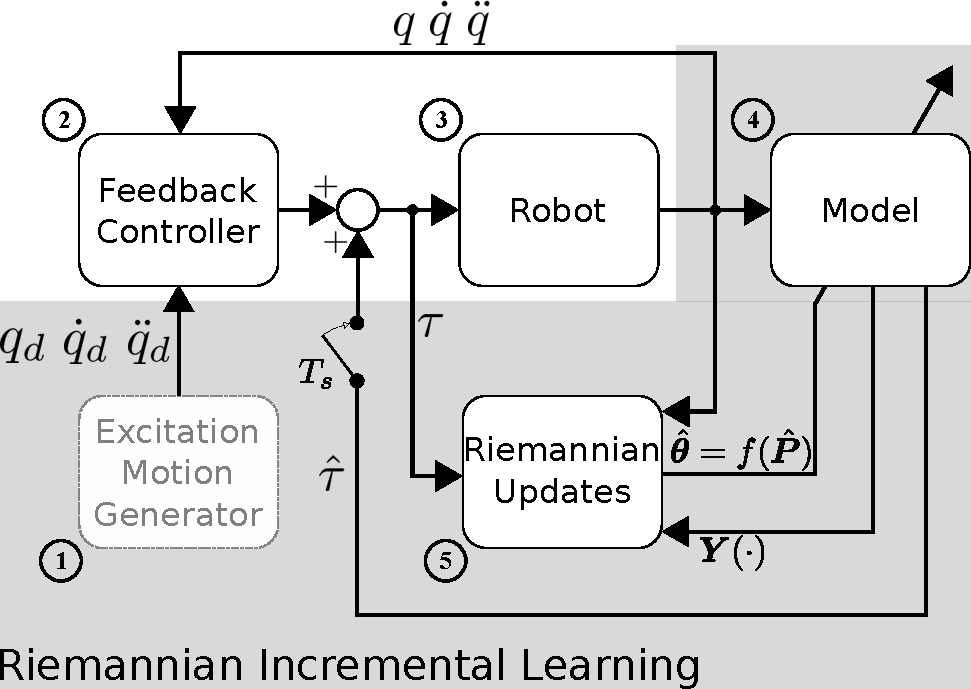
\includegraphics[width= 0.7\columnwidth]{riemannian_incremental_learning.pdf} 
	\hspace*{\fill}
	\caption[] {Overview of the proposed learning scheme.}\label{fig:riemannian_incremental_learning}
\end{figure}
%--- 
%% SUBSECTION ========================================================================================
%\subsection{Riemannian gradient descent on $ \mathcal{S}^{4}_{++} $}
%The \emph{Riemannian gradient} at a point $\bm{P}\in\mathcal{M}$ is the orthogonal projection of the gradient in ambient Euclidean space $\bm{G} = \nabla J(\cdot)=\frac{\partial J}{\partial \bm{P}}\in \mathbb{R}^{n \times n}$ onto $\mathcal{T}_{\bm{P}}\mathcal{M}$ \cite{Boumal2014Optimizationestimationmanifolds.}; that is, 
%$ \text{grad}_{\bm{P}}J(\bm{P}) = \Pi_{ \mathcal{T}_{\bm{P}}}\left(\nabla J(\bm{P})\right) \in \mathcal{T}_{\bm{P}}\mathcal{M} $, with the projection operator defined as $\Pi_{ \mathcal{T}_{\bm{P}}}(\bm{G})\triangleq\bm{P}\left(\frac{\bm{G}+\bm{G}^T}{2}\right)\bm{P},\quad \forall \bm{P}\in \mathcal{M}  $ \cite{Brooks2019Riemannianbatchnormalization}. As described in \cite{Bonnabel2013Stochasticgradientdescent}, Riemannian gradient descent uses $
%\bm{P}^{k+1}= \text{Exp}_{\bm{P}^k}\left(-\gamma \text{grad}_{\bm{P}^k}J(\bm{P}^k)\right)$, $ \gamma \in (0,1]$, to compute the update to the parameter $\bm{P}$ on $\mathcal{M}$. Likewise, the Riemannian gradient of a function $J(\bm{P})$ at a point $\bm{P}=(\bm{P}_1,\ldots,\bm{P}_N)\in\mathcal{M}^N$ is expressed by $
%\text{grad}_{\bm{P}}J=\left(\text{grad}_{\bm{P}_i}J_1, \ldots, \text{grad}_{\bm{P}_N}J_N\right)$;  with $\bm{P}_i\in\mathcal{M}_i$, i.e. defined on a product manifold.
%%
%Here the term $\text{grad}_{\bm{P}_i}J_i$ represents the Riemannian gradient of the partial map $
%J_i:\bm{Q}\in \mathcal{M}_i \mapsto f\left(\bm{P}_1,\ldots,\bm{P}_{i-1},\bm{Q},\bm{P}_{i+1},\ldots,\bm{P}_N\right)$. 
%%---
%\begin{center}
%	\begin{algorithm}[t!]\small
%		\caption{RAMS gradient descent in $\mathcal{M}^N$}\label{alg:rams_gd}
%		\begin{algorithmic}[1]
%			%		\Procedure{Parameter update}{$n$}
%			\State \textbf{Require} $\hat{\bm{P}}(0)\in \mathcal{S}^4_{++}$ initial feasible point
%			\State \textbf{Require} $\beta_1,~\beta_2 \in \left[0,1\right)$ exponential decay rates for moment estimates%\footnote{The standard values for the first momentum term $ \beta = 0.9 $ and second momentum term $ \beta_2 = 0.999 $ are considered.}
%			\State \textbf{Require} $\alpha$~learning rate
%			\State $\bm{P}_t \gets \hat{\bm{P}}(0)$~\Comment{initialization}
%			\State $\bm{m}_t \gets \bm{0}$
%			\State $\bm{\tau}_t \gets \bm{0}$
%			\State $v_t \gets 0$
%			\State $\hat{v}_t \gets 0$
%			\For{$t= 1$ to $T_s$} \Comment{loop over samples}
%			\State $\mathcal{B} \gets  \bm{x}_t $ \Comment{store current sample}
%			%\tikzmark{top}
%			\State Select $ \mathcal{X} $  from $ \mathcal{B} $
%			% \tikzmark{right}
%			\State Compute $ J(\bm{P}\lvert\ \mathcal{X}) $ and $ \text{grad}_{\bm{P}_t}J(\cdot) $					
%			\For{$i=1$ to N} 
%			%\tikzmark{bottom}
%			\State $ \bm{g}^i_t = \text{grad}_{\bm{P}_t}J_i(\bm{P}_t\lvert\ \mathcal{X}) $
%			\State $ \bm{m}^i_t = \beta_1 \bm{\tau}^i_{t-1} + (1 - \beta_1)\bm{g}^i_t $
%			\State $ v^i_t = \beta_2 v^i_{t-1} + (1 - \beta_2) \left\lVert \bm{\bm{g}^i_t} \right\rVert^2_{\bm{P}_t} $
%			\State $ \hat{v}^i_t = \text{max}(\hat{v}^i_{t-1},v^i_t)  $
%			\State $ \bm{P}^i_{t+1}= \text{Exp}^i_{\bm{P}^i_t}\left(- \frac{\alpha}{\sqrt{\hat{\bm{v}}^i_t + \epsilon}}\bm{m}^i_t\right) $
%			\State 	$ \bm{\tau}^i_t = \Gamma^i_{\bm{P}^i_t\to \bm{P}^i_{t+1}}\left(\bm{m}^i_t\right) $
%			\EndFor
%			\EndFor
%			\State \textbf{return} $\bm{P}^i_{t+1}$ for $i=1,\ldots,N$ \Comment{parameter updates}
%		\end{algorithmic}
%		%			\AddNote{top}{bottom}{right}{Replay buffer.}
%	\end{algorithm}
%\end{center}
%%---
%Motivated by the stability and convergence speed of the state-of-the-art online gradient descent algorithm AMSGrad \cite{Reddi2019convergenceADAM}, we now use its manifold version, the Riemannian AMS gradient descent ---RAMSGrad for short \cite{Becigneul2018Riemannianadaptiveoptimization}. \textcolor{black}{Algorithm~\ref{alg:rams_gd} shows the core steps of RAMSGrad, where $ \bm{m}_t $ and $ v_t $ are the moving averages of the gradient and its Riemannian norm. The term $ \bm{\tau}_t $ allows the aggregation of the previous gradients by considering the curvature of the manifold. 	Finally, $ \alpha $ is the initial learning rate. In our implementation, the standard values for the first and second momentum terms are used ($ \beta_1 = 0.9 $, $ \beta_2 = 0.999 $). The algorithm runs up to a final user-defined time $ T_s$. We expand the algorithm introducing an experience replay buffer $ \mathcal{B} $ to break the correlation between consecutive samples by storing $N_{\mathcal{B}}$ previous data points. At every time step $ t $ the current sample $ \bm{x}_t $ is pushed into the buffer by taking the place of a randomly-chosen sample. From $ \mathcal{B} $ a mini batch $ \mathcal{X} $ of $ N_{\mathcal{X}}  $ samples is selected and used to compute the cost $ J(\bm{P}_t \lvert\ \mathcal{X}) $ and its corresponding Riemannian gradient $
%	\text{grad}_{\bm{P}}J$. %This mitigates the temporal correlations of the samples and induces a more \emph{independent and identically distributed} construction of the mini batches.}
%This results in mini batches constructed from \emph{independent and identically distributed} samples with no temporal correlation.}
%
%% ===================================================================================================
%%                                                 |                                                 |
%%                                                 |                                                 |
%% -------------------------------------------- SECTION ---------------------------------------------|
%%                                                 |                                                 |
%%                                                 |                                                 |
%% ===================================================================================================
%\section{Results}
%% SUBSECTION ========================================================================================
%\subsection{Influence of force/torque measurement setups}
%Using a virtual robot with fully determined properties we analyze the influence of different joint force/torque measurement setups on the $ \hat{\bm{\theta}} $ generated by RIL. The robot is made of cylindrical bodies of uniform density and revolute joints that rotate around the z-axis of the corresponding joint frame. Fig.~\ref{fig:cylindrical_robot} shows the structure of the robot together with the actual inertia ellipsoids for all its links. To generate motion data, a set of pre-computed excitation trajectories was given to the manipulator and the joint wrenches were computed using the recursive Newton-Euler algorithm. RIL was used to generate Riemannian updates based on \eqref{eq:dyn_cost_func_manifold} and starting from $ {\hat{\bm{P}}_i(0)}_{i=1}^N = \bm{I}_{4\times4}$ (identity matrix), i.e. \textbf{prior information is neither used nor required}. Additionally, we set the replay buffer $ \mathcal{B} $ to  hold $ N_{\mathcal{B}} =5$ samples and a mini batch $ \mathcal{X} $ with size equal to the buffer size. We contemplate three different force/torque measurement setups as supervisory signals: (a) joint wrench, (b) wrench at the first joint and all subsequent joint torques, and (c) only joint torques. Figure~\ref{fig:cylindric_robot_estimated_structure} shows the resulting inertia ellipsoids for each setup. Clearly, wrench measurements (see Fig.~\ref{fig:cylindrical_robot_wrench}) lead to parameters that closely resemble ground truth. In contrast, with joint torques only, it is not possible to fully reproduce the original set, as seen noticeably by the wanting estimations of the proximal links. Nonetheless, estimates for the distal-most links do approximate the real values. Finally, the information provided by a force/torque sensor at the first joint results in improvements to the location of the center of mass of the proximal links, see  Fig.~\ref{fig:cylindrical_robot_wrenchTorque}. To the right of Figs.~\ref{fig:cylindrical_robot_wrench} to \ref{fig:cylindrical_robot_wrenchTorque}, the results of learning when choosing $ \hat{\bm{P}}(0) = \bm{P}^*(1 + \bm{\epsilon})$, where  $ \bm{P}^* $ are the actual values and $ \bm{\epsilon} \sim \mathcal{N}(0,0.5)$ is a small perturbation, are displayed. This shows that, when the initial values are in the vicinity of the real values, RIL will induce negligible changes.
%%---
%\begin{figure}
%\centering	
%\hspace*{\fill}
%\subfloat[]{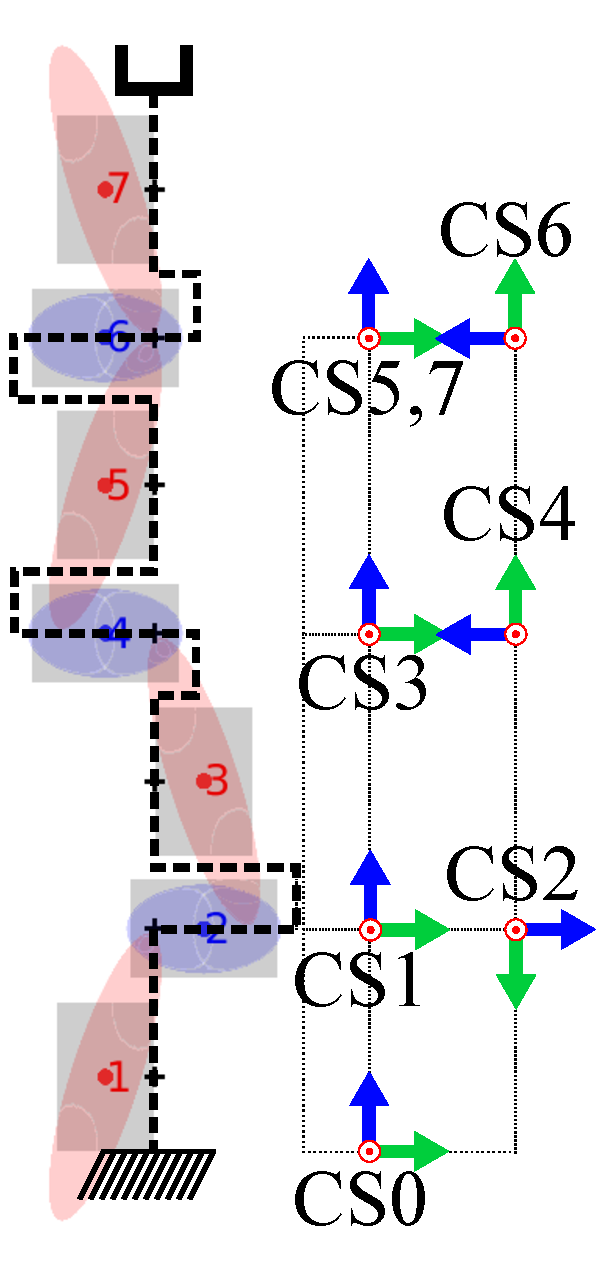
\includegraphics[width= 0.23\columnwidth]{fig/cylindrical_robot_update.pdf} \label{fig:cylindrical_robot}}
%\hspace*{-0.9em}
%\subfloat[]{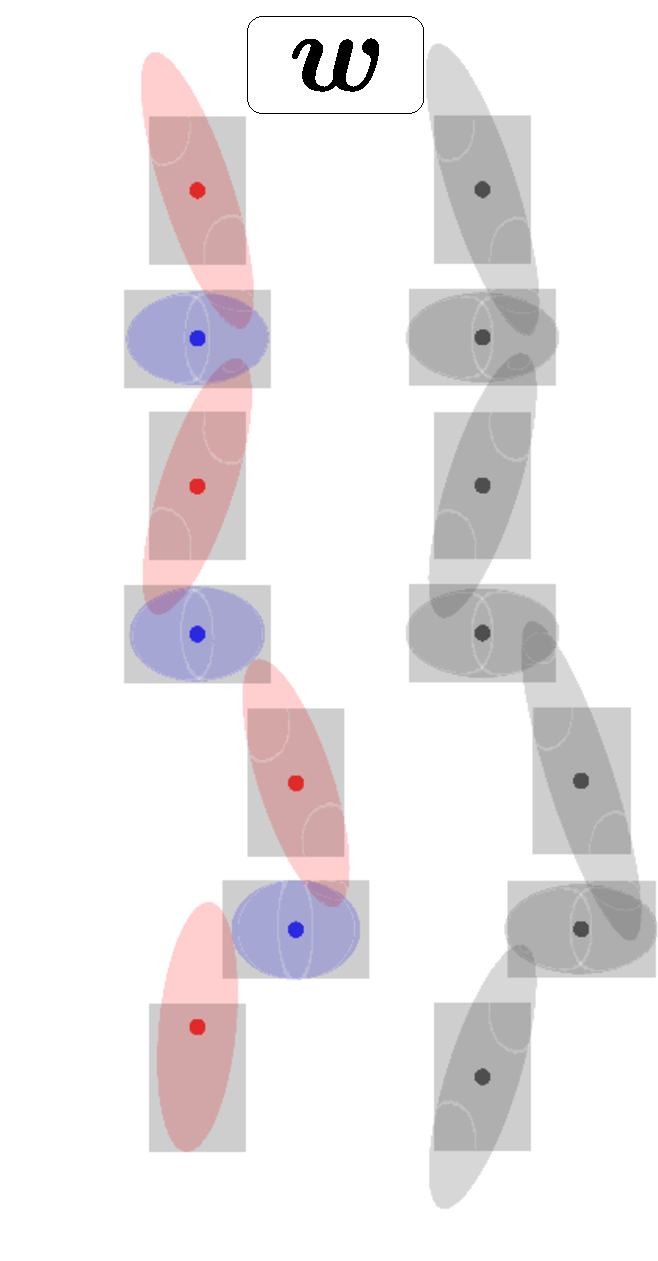
\includegraphics[width= 0.25\columnwidth]{fig/cylbot_wrench_v2.pdf} \label{fig:cylindrical_robot_wrench}}
%\hspace*{-0.9em}
%\subfloat[]{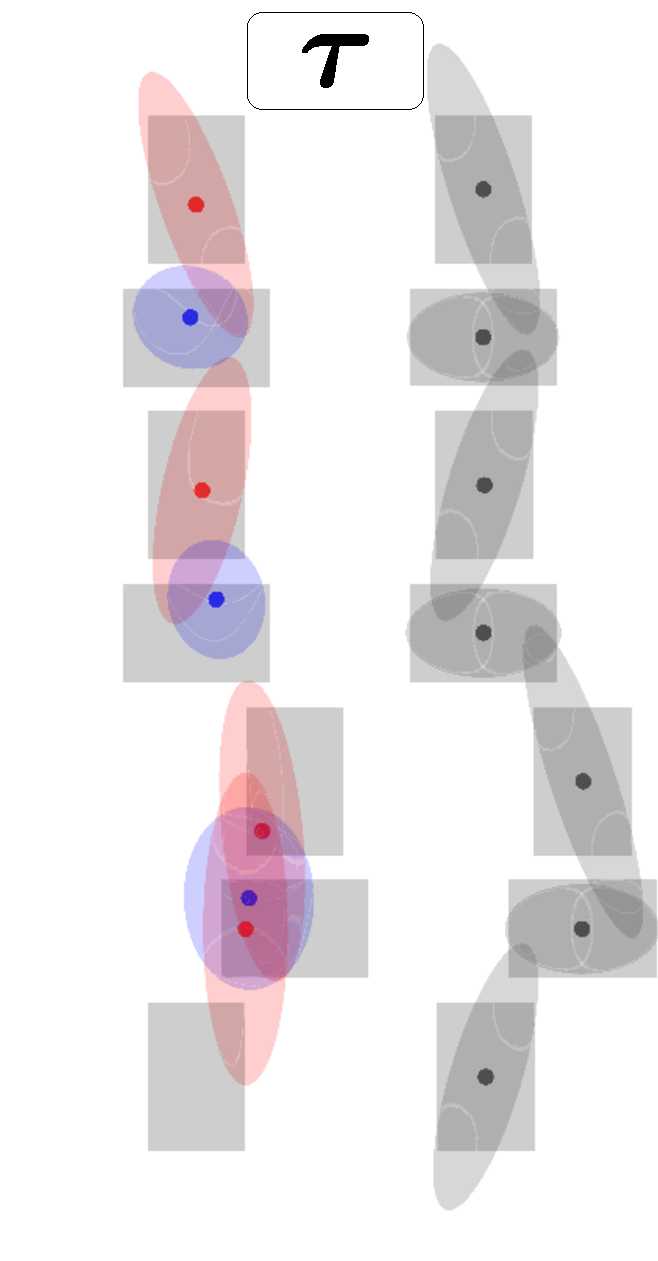
\includegraphics[width= 0.25\columnwidth]{fig/cylbot_torque_v2.pdf} \label{fig:cylindrical_robot_torque}}
%\hspace*{-0.9em}
%\subfloat[]{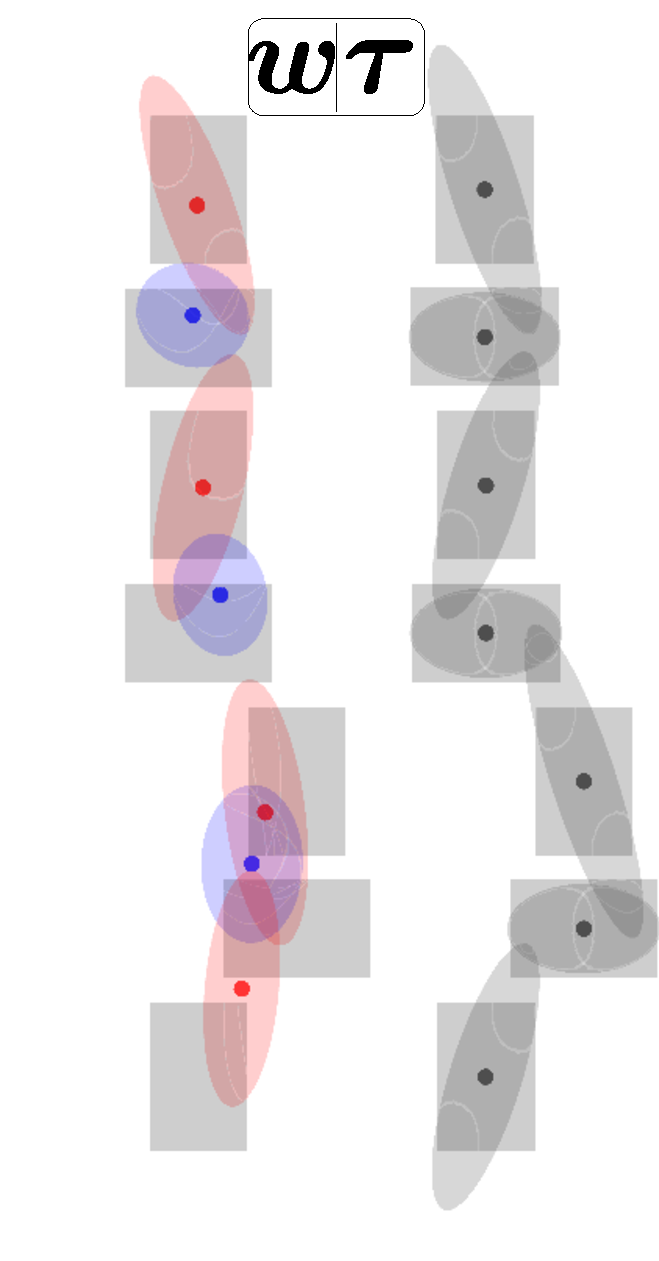
\includegraphics[width= 0.25\columnwidth]{fig/cylbot_wrench_torque_v2.pdf} \label{fig:cylindrical_robot_wrenchTorque}}			
%\hspace*{\fill}
%\caption[] {\label{fig:cylindric_robot_estimated_structure} A robot with cylindrical links and their corresponding inertial ellipsoids: \subref{fig:cylindrical_robot} actual structure, estimation using \subref{fig:cylindrical_robot_wrench} joint wrench ($ \bm{w} $), \subref{fig:cylindrical_robot_torque} joint torque only ($ \bm{\tau} $), \subref{fig:cylindrical_robot_wrenchTorque} first joint wrench and the torques from subsequent joints ($ \bm{w}|\bm{\tau} $).}
%\end{figure}
%%---
%% SUBSECTION ========================================================================================
%\subsection{Simulated Franka Emika Panda}
%Now we consider a model of a state-of-the-art 7 DoF collaborative robot, the Franka Emika Panda. For this we take as ground truth the inertial parameters reported in \cite{Gaz2019Dynamicidentificationfranka}, found using classical system identification (SID), and use the Newton-Euler approach to simulate the forward and inverse dynamics of the robot.  In the experiment the manipulator executes repeatedly a series of pre-computed excitation trajectories composed of the sum of a Fourier series and a polynomial, as described in \cite{Park2006Fourierbasedoptimal}. Additionally, the end-effector holds a load to generate significant joint torques at the distal joints.  RIL is then used to learn the parameters and evaluate how they compare to the values reported in \cite{Gaz2019Dynamicidentificationfranka}. This time we set $ N_{\mathcal{B}}=$1000 for the replay buffer. 
%% ---------------------------------------------------------------------------------------------------
%\subsubsection{Change in load}
%To evaluate if RIL can adapt to structural changes an experiment was performed in which the test load ($ m_L = \unit[1.45]{kg} $) was learned as part of the manipulator's body and was then suddenly removed. This resembles an abrupt change in the dynamic properties. The experiment allowed us to see how fast RIL can adapt to such changes. The test ran for 1000 seconds with the load being removed at $ t = \unit[700]{s} $. Fig.~\ref{fig:load_drop_mass_estimates} shows the estimates from RIL for all the masses. We chose to focus on the link masses to address one potential limitation: the dependence on proprioception. Taking the seventh link's mass as example ($m_7 = \unit[1.46]{kg} $), it can be seen that while the load is held, the estimation of the compound mass is reasonably good; i.e. $ \hat{m}_7 \simeq m_7 + m_L $. When the load is removed, a large difference between the actual mass and the estimated mass is evident ($\hat{m}_7< \unit[1]{kg}$). Although the learning metric $ J(\cdot) $ is still minimized, it obviously deviates from reality. The cause of this is that RIL depends on proprioceptive information, i.e. joint measurements. In particular, without a test load, the torque at the seventh joint is considerably small in relation to the rest, a fact that naturally complicates the correct learning of the 7th link parameters.
%%---
%\begin{figure}[t!]
%\centering
%\hspace*{\fill}
%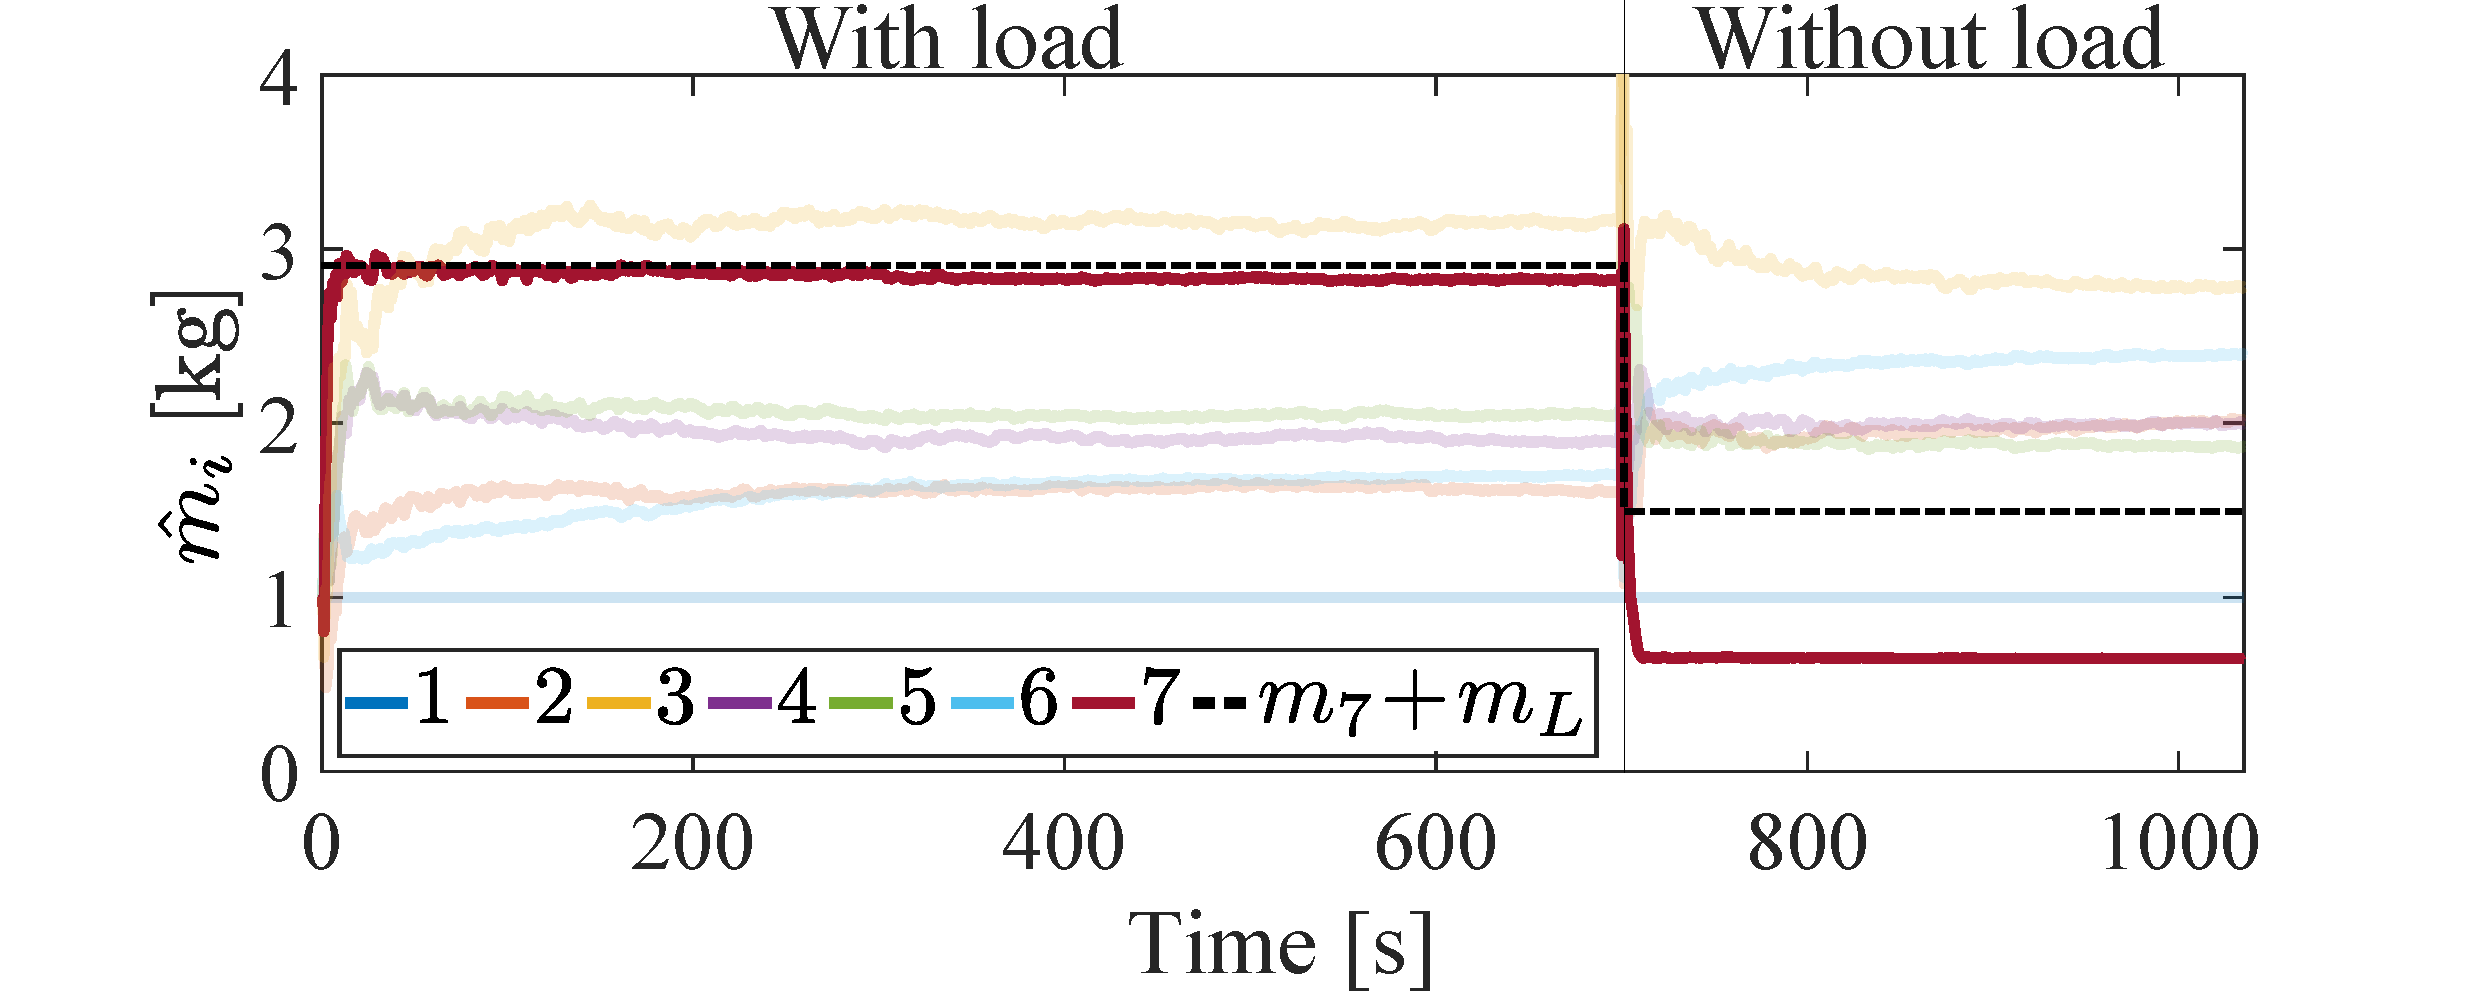
\includegraphics[width= 0.99\columnwidth]{fig/load_drop_mass_estimates_annotated_v3.pdf} 
%\hspace*{\fill}
%\caption[] {Relearning of the robot's link masses.}\label{fig:load_drop_mass_estimates}
%\end{figure}
%%---
%% ---------------------------------------------------------------------------------------------------
%\subsubsection{Comparison to a similar method}
%We implemented the natural adaptive controller (NAC) introduced in \cite{Lee2018naturaladaptivecontrol} to track the same excitation trajectory. In this method a Riemannian metric is used to derive a passibity-based parameter adaption law that uses natural gradient descent. This work directly compares to ours in that it deals with online estimation and physical feasibility. After a period of 1000 seconds the parameters were considered learned. Three aspects are of interest to us: the quality of the estimated parameters, their feasibility and the accuracy of the inverse dynamics torques that result from them. The former two points can be addressed by looking at the estimated mass and the eigenvalues of the density weighted covariance matrix for all links (i.e. $m_i$ and $ \lambda(\bm{\Sigma}_i) $) for methods RIL and NAC and comparing them against those from SID. In Table~\ref{tab:panda_simulation_results} we show the parameters grouped in the vector $ \bm{p}_i= [m, \lambda_1, \lambda_2, \lambda_3]^T  $ for all links for the three cases. Notice that feasibility is ensured as both, NAC and RIL, produced positive values. To evaluate the accuracy and generalizability of the inverse dynamics torques, we computed them for a new unseen trajectory using the (ground truth) parameters from SID and the estimated parameters from RIC and NAC and calculated the corresponding mean squared error,  $ J(\cdot) $, as defined in \eqref{eq:dyn_cost_func_euclidean}. Table~\ref{tab:panda_simulation_results} shows that $ J_{RIL} $  was orders of magnitude smaller than $ J_{NAC} $ at final time.
%%---
%\begin{table}[!t]
%\caption{Parameter feasibility and mean squared error for NAC and RIL relative to SID.}
%\centering
%\tiny
%\resizebox{\columnwidth}{!}{
%	\begin{tabular}{ p{0.05cm}p{0.2cm}p{0.3cm}p{0.3cm}p{0.3cm}p{0.3cm}p{0.3cm}p{0.3cm}p{0.3cm}p{0.5cm}}
%		\label{tab:panda_simulation_results}
%		& $\boldsymbol{p}$ & Link 1 & Link 2 & Link 3 & Link 4 & Link 5 & Link 6 & Link 7 & $J(\cdot)$\\    \hline
%		\multirow{4}{*}{\STAB{\rotatebox[origin=c]{90}{SID}}} & $m_i$	&	4.971	&	0.647	&	3.229	&	3.588	&	1.226	&	1.667	&	2.915	& \multirow{4}{*}{\STAB{\rotatebox[origin=c]{0}{N/A}}}\\
%		&$\lambda_{1}$	&	0.745	&	0.028	&	0.047	&	0.072	&	0.031	&	0.010	&	0.131 &	\\
%		&$\lambda_{2}$	&	0.006	&	0.003	&	0.016	&	0.012	&	0.010	&	0.002	&	0.018 &	\\
%		&$\lambda_{3}$	&	0.002	&	0.000	&	0.001	&	0.005	&	0.000	&	0.001	&	0.003 &	\\ \hline
%		\multirow{4}{*}{\STAB{\rotatebox[origin=c]{90}{NAC}}} & $m_i$	&	1.000	&	1.897	&	2.257	&	2.670	&	2.240	&	1.828	&	2.790	& \multirow{4}{*}{0.0037}\\
%		&$\lambda_{1}$	&	0.200	&	0.081	&	0.071	&	0.092	&	0.101	&	0.027	&	0.118 &	\\
%		&$\lambda_{2}$	&	0.015	&	0.021	&	0.019	&	0.013	&	0.007	&	0.007	&	0.010 &	\\
%		&$\lambda_{3}$	&	0.015	&	0.015	&	0.013	&	0.012	&	0.006	&	0.007	&	0.005 &	\\ \hline
%		\multirow{4}{*}{\STAB{\rotatebox[origin=c]{90}{RIL}}} & $m_i$	&	1.000	&	1.610	&	3.162	&	1.897	&	2.047	&	1.703	&	2.822 & \multirow{4}{*}{\textbf{9.7E-5}}	\\
%		& $\lambda_{1}$	&	1.000	&	0.073	&	0.048	&	0.121	&	0.098	&	0.025	&	0.120 &	\\
%		& $\lambda_{2}$	&	0.003	&	0.024	&	0.017	&	0.012	&	0.005	&	0.006	&	0.011 &	\\
%		& $\lambda_{3}$	&	0.003	&	0.009	&	0.006	&	0.008	&	0.003	&	0.005	&	0.003 &	\\
%		\hline
%\end{tabular}}
%\end{table}
%%---
%% ---------------------------------------------------------------------------------------------------
%\subsubsection{Comparison to neural networks}
%Today, neural networks (NN) are the flagship method for data-driven learning. For completeness, we briefly discuss the implementation of a simple NN to learn the inverse dynamics torque of the seventh links using the joint position, velocity and acceleration from all seven joints. A NN with two hidden layers, each having a 100 rectified linear units (ReLU), was used. We fed the NN the same 1000 seconds worth of data  seen by RIL and NAC as training data set and test for generalization on the same unseen trajectory. The results for the test, validation and training sets are shown in Table~\ref{tab:nn_results}. The results from the test set are far from satisfactory when compared to RIL on the same number of samples. Naturally, other architectures and networks (such as LSTMs \cite{Rueckert2017Learninginversedynamics} and recurrent NN \cite{Polydoros2017Onlinemultitarget}) could be used to learn inverse dynamics, but they always involve many hyperparameters and demand large amounts of data. Apart from this limitation, the lack of interpretability of the model is striking; e.g., the tested NN has 12,200 tunable parameters that provide no useful information about the system.
%%---
%\begin{table}[!t]
%\caption{Results using a neural network.}
%\vspace{-2ex}
%\begin{center}
%	\begin{tabular}[b]{p{1cm}p{1cm}p{1cm}} 
%		\hline
%		\textbf{$ J_{train} $} & $ J_{val} $ &  $ J_{test} $ \\ 			
%		\hline
%		0.042	  & 0.05 & 0.59\\
%		\hline
%	\end{tabular}
%\end{center}
%\label{tab:nn_results}
%\end{table}
%%---
%% SUBSECTION ========================================================================================
%\subsection{Test on a real Franka Emika Panda}
%We use RIL to learn the inertial parameters of a real Franka Emika Panda 7-DoF manipulator. Once again, the experiment consisted on the robot following repeatedly a precomputed 30 seconds excitation trajectory while holding an external load to excite the torques at the distal joints. The robot was driven by a built-in velocity tracking controller. Measurement data from the robot was recorded at a rate of 1 kHz and included joint angle and torque. Joint velocity was obtained using numerical differentiation. As for joint acceleration, since there is no direct measurement for it, the desired values were taken instead under the assumption that the controller achieves a small tracking error (i.e. $ \ddot{\bm{q}} \approx \ddot{\bm{q}}_{ref}$). Since we \textbf{do not} make assumptions about the inertial properties of the links \textbf{nor} have any initial values taken from a CAD software or any other source, we select once again the initial guess $ \hat{\bm{P}}_0 $ as an identity matrix for all links. Regarding RAMSGrad hyperparameters, we took the defaults values for $ \beta_1 = 0.9 $ and $ \beta_2 = 0.999 $ and settled for a learning rate $ \alpha = 0.01 $. Since we focus on trying to find the parameters of the robot, we provide information to the algorithm about the inertial properties of the load. 
%
%% SUBSECTION ========================================================================================
%\subsubsection{Impact of noise}\label{sec:results}
%%\textcolor{red}{We observed that RAMSGrad was particularly sensitive to noise as it hindered parameter convergence introducing high variability in the updates. To combat this we increased the size of the replay buffer and the mini batches to $N_{\mathcal{B}} = 10000$ and $N_{\mathcal{X}} = 5$. With this strategy it was possible to shrink the parameter update variability and elucidate a convergence trend. Fig.~\ref{fig:results_panda} shows this trend in the parameters of interest to evaluate physical feasibility (an exponential moving average was superimposed on the plots to facilitate readability); i.e. mass and eigenvalues of the density weighted covariance matrix $ \bm{\Sigma} $. As all values are positive at all times, then \emph{feasibility is ensured}.	As for the learned inertia ellipsoids, similar to the case study, the distal-most links were better estimated, with the proximal links suffering from identifiability limitations and lack of excitation.}
%\textcolor{black}{We observed that RAMSGrad was particularly sensitive to noise as it hindered parameter convergence introducing high variability in the updates. To combat this we increased the size of the replay buffer to $N_{\mathcal{B}} = 10000$ keeping the mini batch size as $N_{\mathcal{X}} = 5$. With this strategy it was possible to shrink the parameter update variability and reveal a convergence trend.}
%% ---------------------------------------------------------------------------------------------------
%\subsubsection{Comparison to system identification}
%Figs.~\ref{fig:panda_ril_parameters} and \ref{fig:panda_sid_parameters} report the full set of inertial parameters obtained from RIL and SID. Although we cannot fully learn the parameters of proximal links since it is a fixed-base robot, RIL was able to learn a more consistent description of the second link, as the mass found in  SID  is comparatively too small (considering that the first two links are structurally similar). The remaining masses are comparable in both methods. As for the remaining parameters, a qualitative assessment can be made by looking at the resulting inertial ellipsoids shown in Figs.~\ref{fig:panda_ril_parameters} and \ref{fig:panda_sid_parameters}. The distal-most links were better estimated, with the proximal links suffering from identifiability limitations and lack of excitation. While both sets satisfy full physical feasibility, there are differences in how well the ellipsoids represent their corresponding link. For instance, as joint motors represent a large part of the link mass, it is expected that the center of mass will be close to the joint location\footnote{Please note that the method followed in \cite{Gaz2019Dynamicidentificationfranka} considered a numerical model of the robot manipulator available from the robot interface, thus, additional information that is not available in our online learning setting.}. Looking at the inertia ellipsoids, it seems that RIL learns a better representation of the inertial parameters of the distal-most links (links 5-7), based on their orientation and center point location. In contrast, the parameters for links 3 and 4 obtained from the system identification process are more consistent (both ellipsoids are comparable in size, as expected from the actual shape of the links). Finally, estimation of the proximal links was unsatisfactory as both methods struggle to generate a good representation for the first link, even though RIL was able to learn a more reasonable mass for link 2. 
%%---
%\begin{figure}[!t]
%\begin{tabular}{m{1.5cm} m{3cm}}
%	\centering
%	\tiny
%	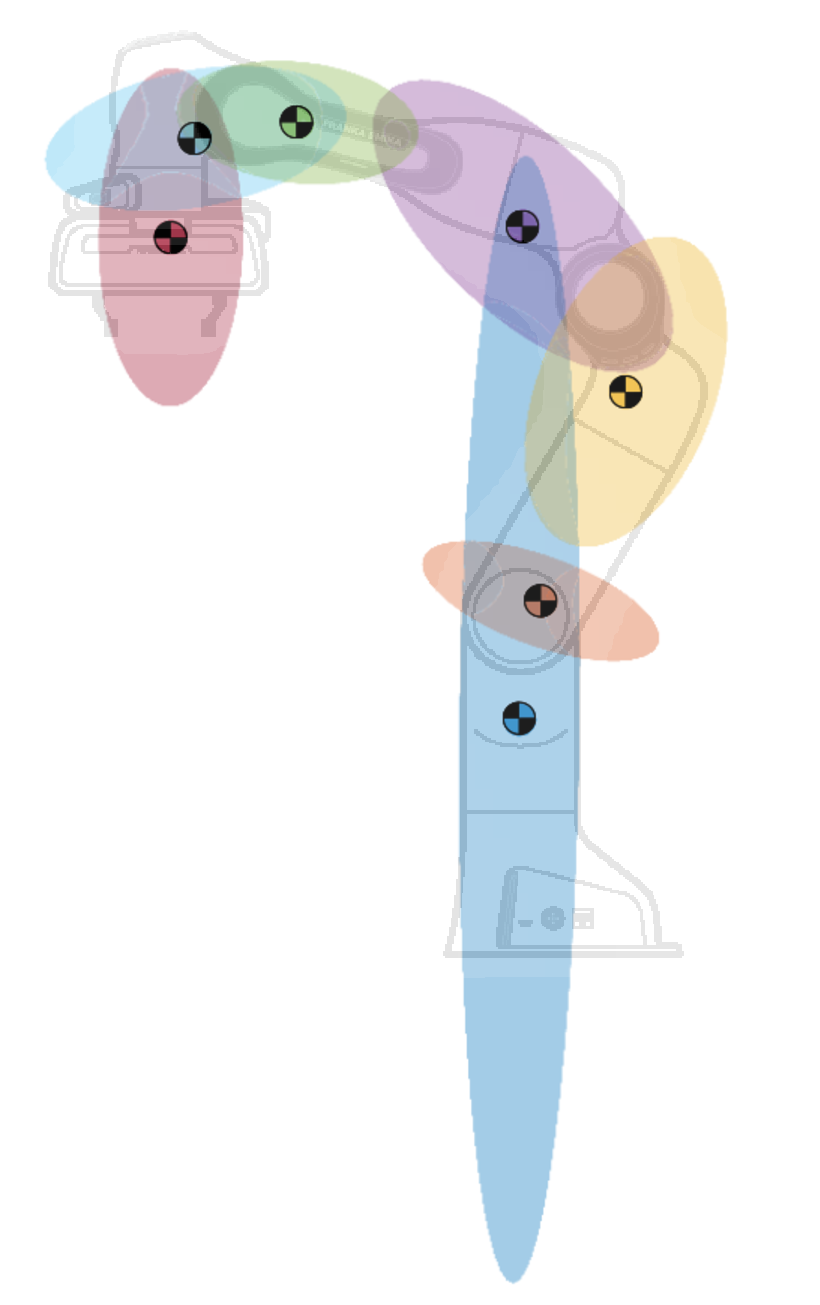
\includegraphics[width = 0.25\columnwidth]{fig/panda_ellipsoid_estimates_sid.pdf} 
%	&
%	\resizebox{0.75\columnwidth}{!}{
%		\begingroup
%		\setlength{\tabcolsep}{1pt} % Default value: 6pt
%		%\renewcommand{\arraystretch}{1.5} % Default value: 1
%		\tiny
%		\begin{tabular}[b]{p{0.6cm}p{0.6cm}p{0.6cm}p{0.6cm}p{0.6cm}p{0.6cm}p{0.6cm}p{0.6cm}}
%			$\boldsymbol{\theta}$ & Link 1 & Link 2 & Link 3 & Link 4 & Link 5 & Link 6 & Link 7\\    \hline
%			$m_i$	&	4.9707	&	0.6469	&	3.2286	&	3.5879	&	1.2259	&	1.6666	&	1.4655	\\
%			$m_iX_{i}$	&	0.0193	&	-0.0020	&	0.0888	&	-0.1908	&	-0.0147	&	0.1002	&	0.0004	\\
%			$m_iY_{i}$	&	0.0103	&	-0.0186	&	0.1267	&	0.3746	&	0.0503	&	-0.0235	&	-0.0031	\\
%			$m_iX_{i}$	&	-0.4654	&	0.0023	&	-0.2147	&	0.0985	&	-0.0471	&	-0.0175	&	0.1453	\\
%			$XX_i$	&	0.7470	&	0.0085	&	0.0565	&	0.0677	&	0.0394	&	0.0025	&	0.0308	\\
%			$XY_i$	&	-0.0002	&	-0.0040	&	-0.0082	&	0.0277	&	-0.0015	&	0.0015	&	0.0004	\\
%			$XZ_i$	&	0.0086	&	0.0103	&	-0.0055	&	0.0039	&	-0.0046	&	-0.0001	&	-0.0007	\\
%			$YY_i$	&	0.7503	&	0.0281	&	0.0529	&	0.0324	&	0.0315	&	0.0106	&	0.0284	\\
%			$YZ_i$	&	0.0201	&	0.0008	&	-0.0044	&	-0.0016	&	0.0022	&	0.0001	&	-0.0005	\\
%			$ZZ_i$	&	0.0092	&	0.0265	&	0.0182	&	0.0776	&	0.0109	&	0.0118	&	0.0067	\\
%			\hline
%		\end{tabular}
%		\endgroup
%	}
%\end{tabular}
%\caption{Inertial parameters and ellipsoids from SID.}\label{fig:panda_ril_parameters}
%\end{figure}
%%---
%\begin{figure}[!t]
%\begin{tabular}{m{1.5cm} m{3cm}}
%	\centering
%	\tiny
%	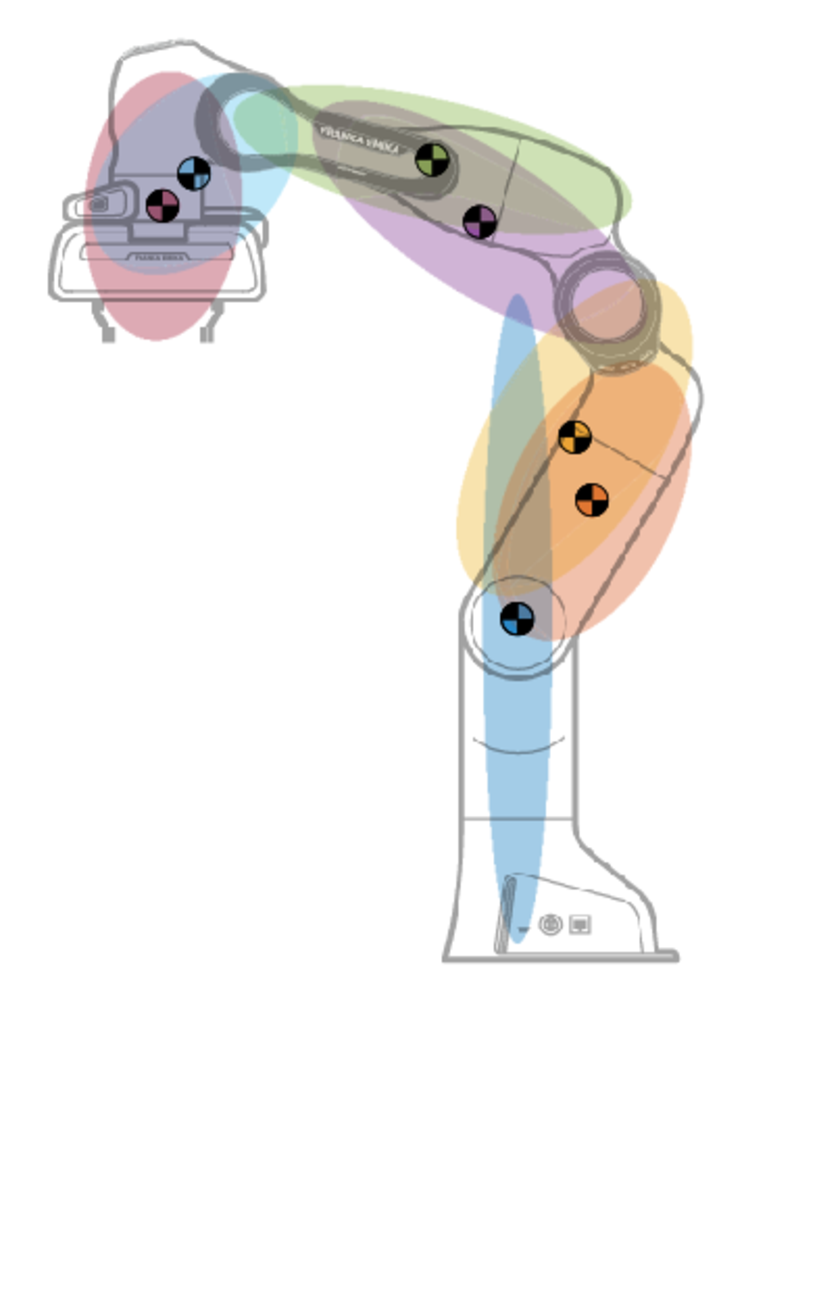
\includegraphics[width= 0.25\columnwidth]{fig/panda_ellipsoid_estimates_ril.pdf} 
%	&
%	\resizebox{0.75\columnwidth}{!}{
%		\begingroup
%		\setlength{\tabcolsep}{1pt} % Default value: 6pt
%		%\renewcommand{\arraystretch}{1.5} % Default value: 1
%		\tiny
%		\begin{tabular}[b]{p{0.6cm}p{0.6cm}p{0.6cm}p{0.6cm}p{0.6cm}p{0.6cm}p{0.6cm}p{0.6cm}}
%			$\boldsymbol{\theta}$ & Link 1 & Link 2 & Link 3 & Link 4 & Link 5 & Link 6 & Link 7\\    \hline
%			$m_i$	&	1.000	&	2.6473	&	3.1301	&	2.4053	&	1.8933	&	1.9949	&	1.4170	\\
%			$m_iX_{i}$	&	0.000	&	-0.0143	&	0.1289	&	-0.1090	&	-0.0209	&	0.1173	&	0.0013	\\
%			$m_iY_{i}$	&	0.000	&	-0.3686	&	-0.0052	&	0.3392	&	0.0289	&	-0.1009	&	0.0139	\\
%			$m_iX_{i}$	&	0.000	&	0.0673	&	-0.4106	&	-0.0002	&	-0.3443	&	-0.0451	&	0.0774	\\
%			$XX_i$	&	1.006	&	0.0998	&	0.1051	&	0.1067	&	0.1078	&	0.0182	&	0.0161	\\
%			$XY_i$	&	0.000	&	0.0049	&	0.0000	&	0.0300	&	0.0003	&	0.0066	&	-0.0001	\\
%			$XZ_i$	&	0.000	&	-0.0029	&	0.0018	&	0.0000	&	-0.0035	&	0.0030	&	-0.0028	\\
%			$YY_i$	&	1.006	&	0.0348	&	0.1179	&	0.0250	&	0.1065	&	0.0190	&	0.0183	\\
%			$YZ_i$	&	0.000	&	0.0161	&	-0.0031	&	-0.0022	&	0.0044	&	-0.0022	&	-0.0006	\\
%			$ZZ_i$	&	0.012	&	0.1020	&	0.0249	&	0.1169	&	0.0099	&	0.0243	&	0.0099	\\
%			\hline
%		\end{tabular}
%		\endgroup
%	}
%\end{tabular}
%\caption{Inertial parameters and ellipsoids from RIL.}\label{fig:panda_sid_parameters}
%\end{figure}
%%---
%% ---------------------------------------------------------------------------------------------------
%\subsubsection{Inverse dynamics estimation}\label{sec:inv_dyn_estimation}
%%---
%\begin{figure*}[t!]
%\centering
%\hspace*{\fill}
%\subfloat[]{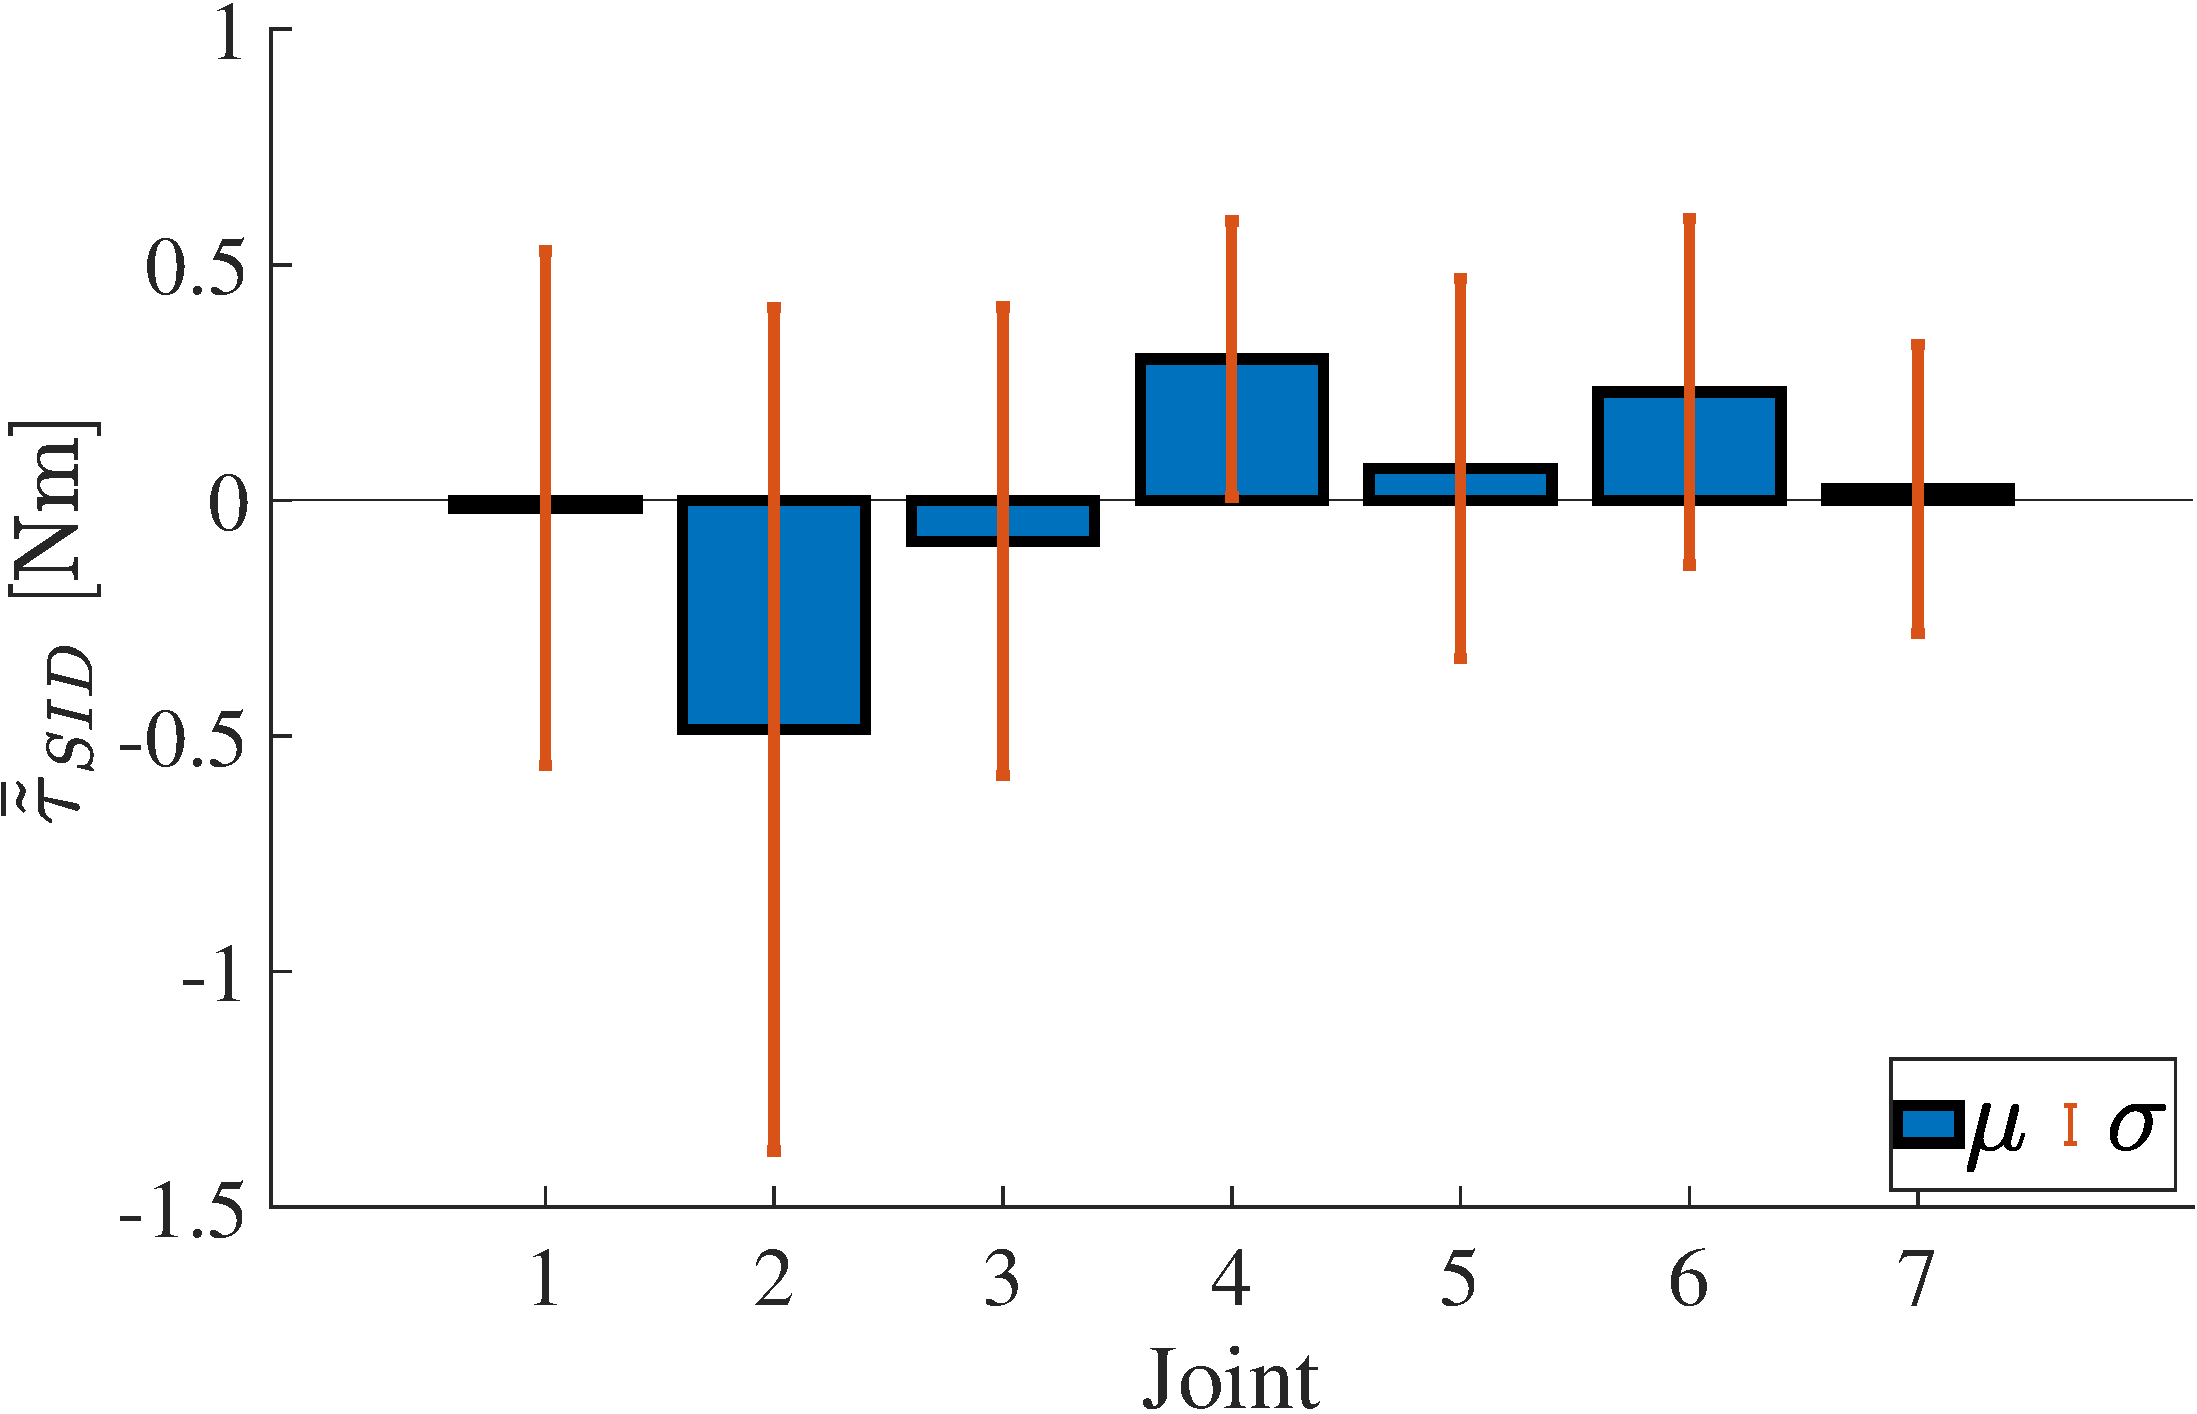
\includegraphics[width= 0.23\textwidth]{fig/panda_torque_sid_abs_error.pdf} \label{fig:panda_torque_error_sid_statistics}}
%\hspace{-0.2em}
%\subfloat[]{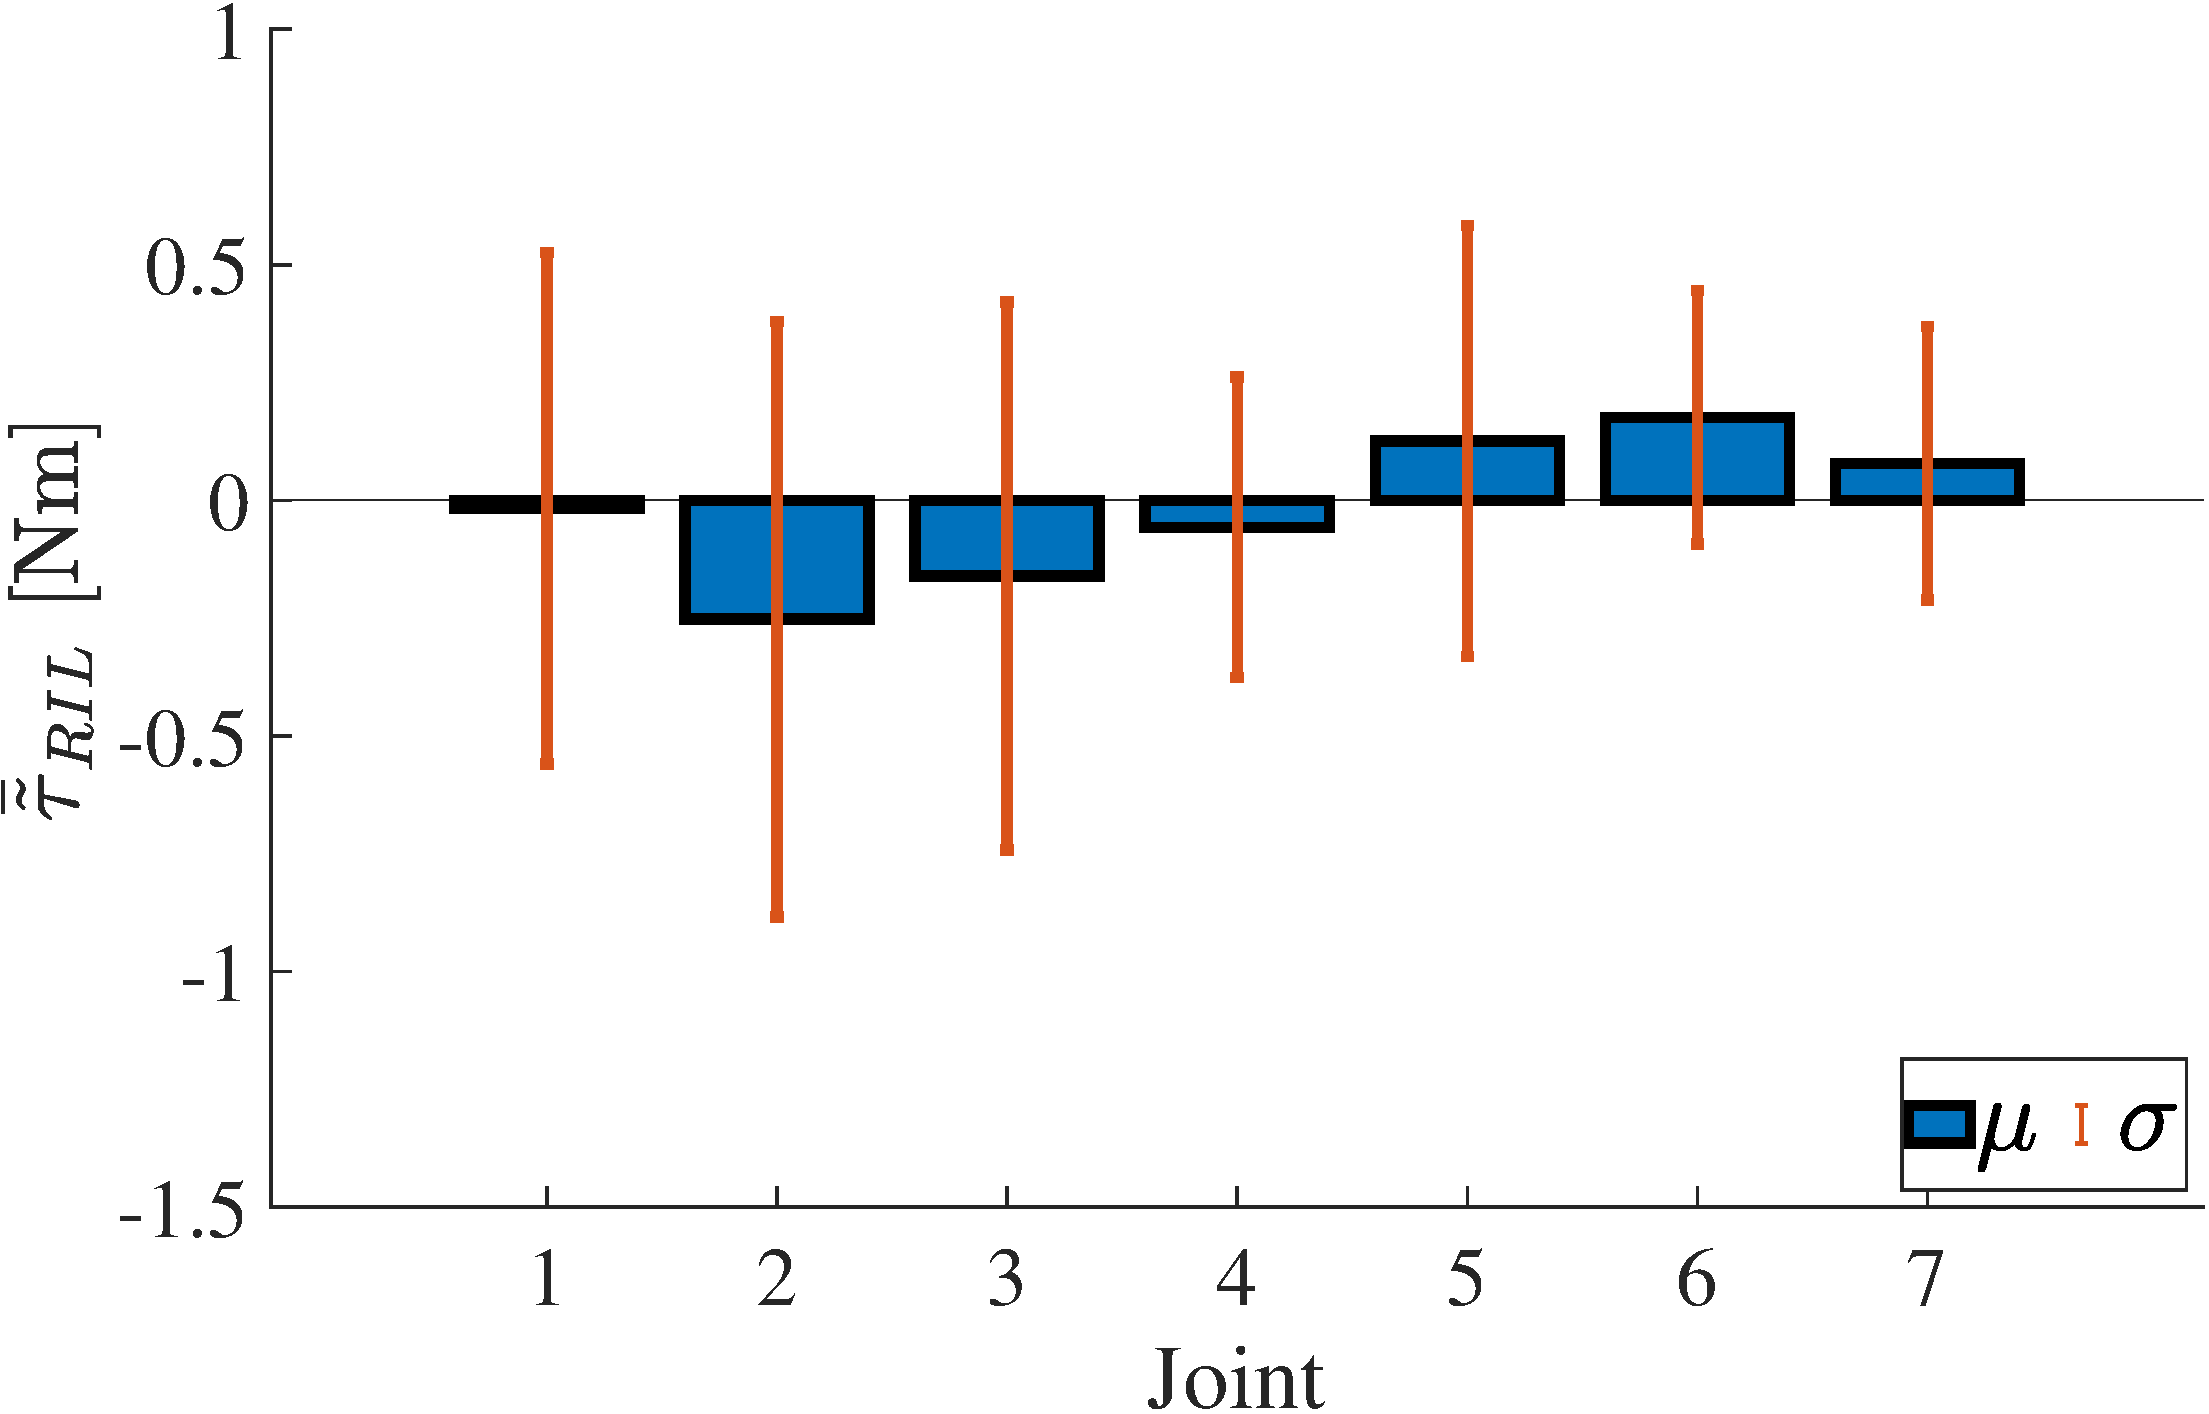
\includegraphics[width= 0.23\textwidth]{fig/panda_torque_ril_abs_error.pdf} \label{fig:panda_torque_error_ril_statistics}}			
%\hspace{-0.2em}
%\subfloat[]{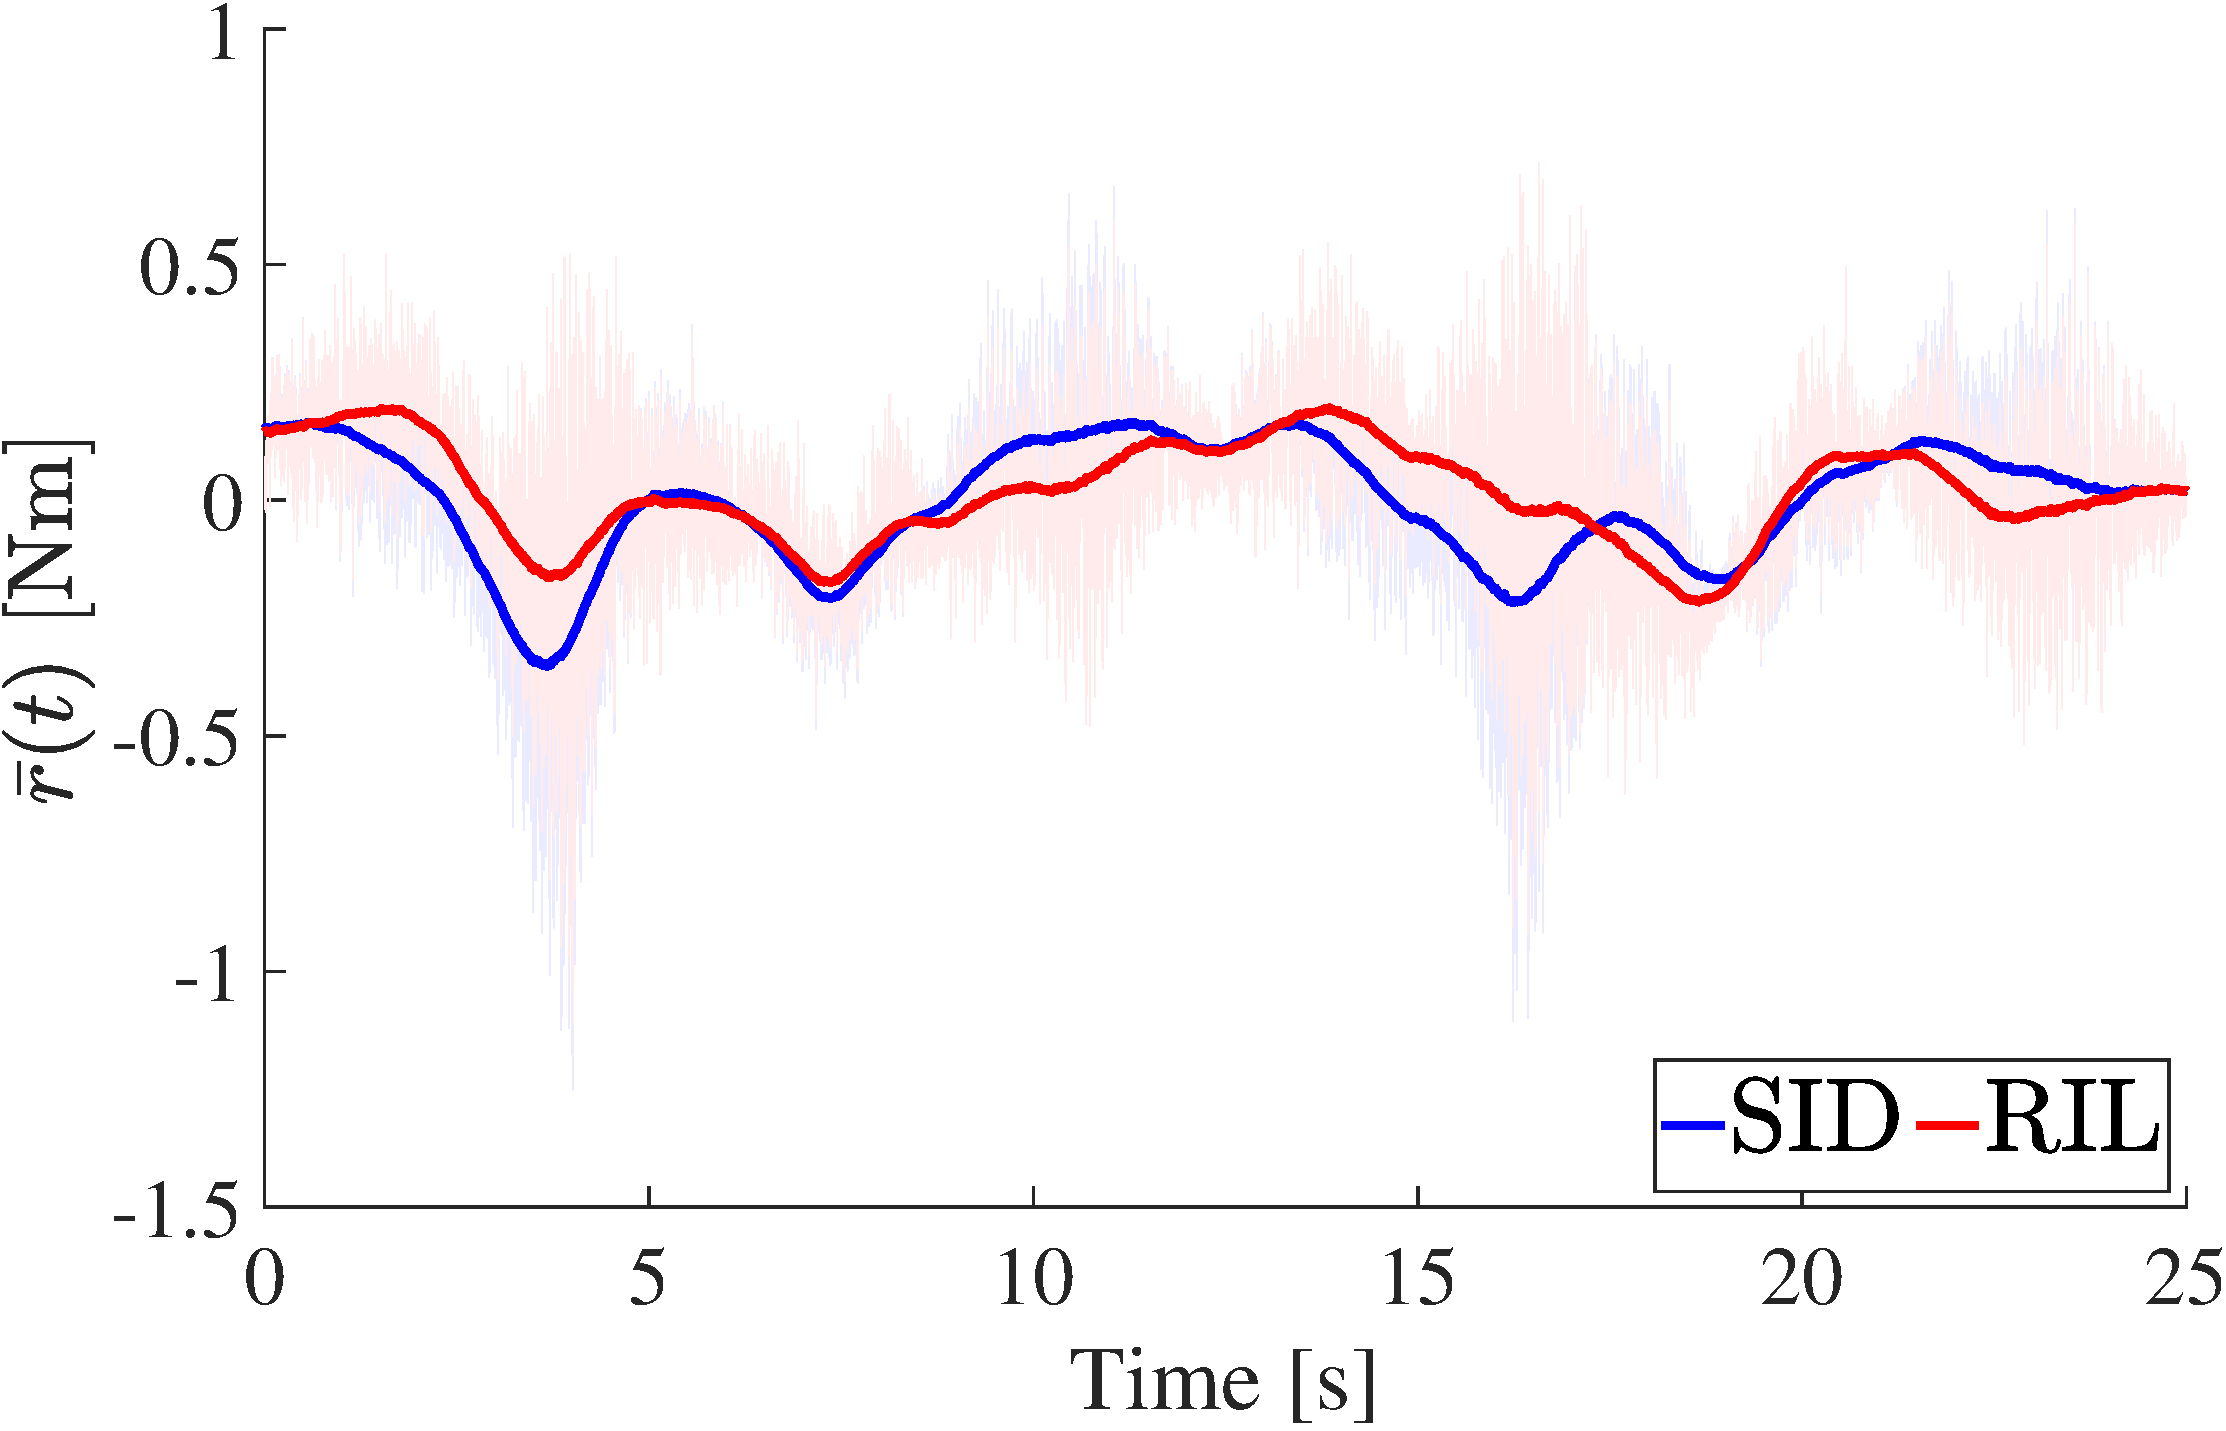
\includegraphics[width= 0.23\textwidth]{fig/momentum_residual_average.pdf} \label{fig:momentum_residual_average}}	
%\hspace{-0.2em}
%\subfloat[]{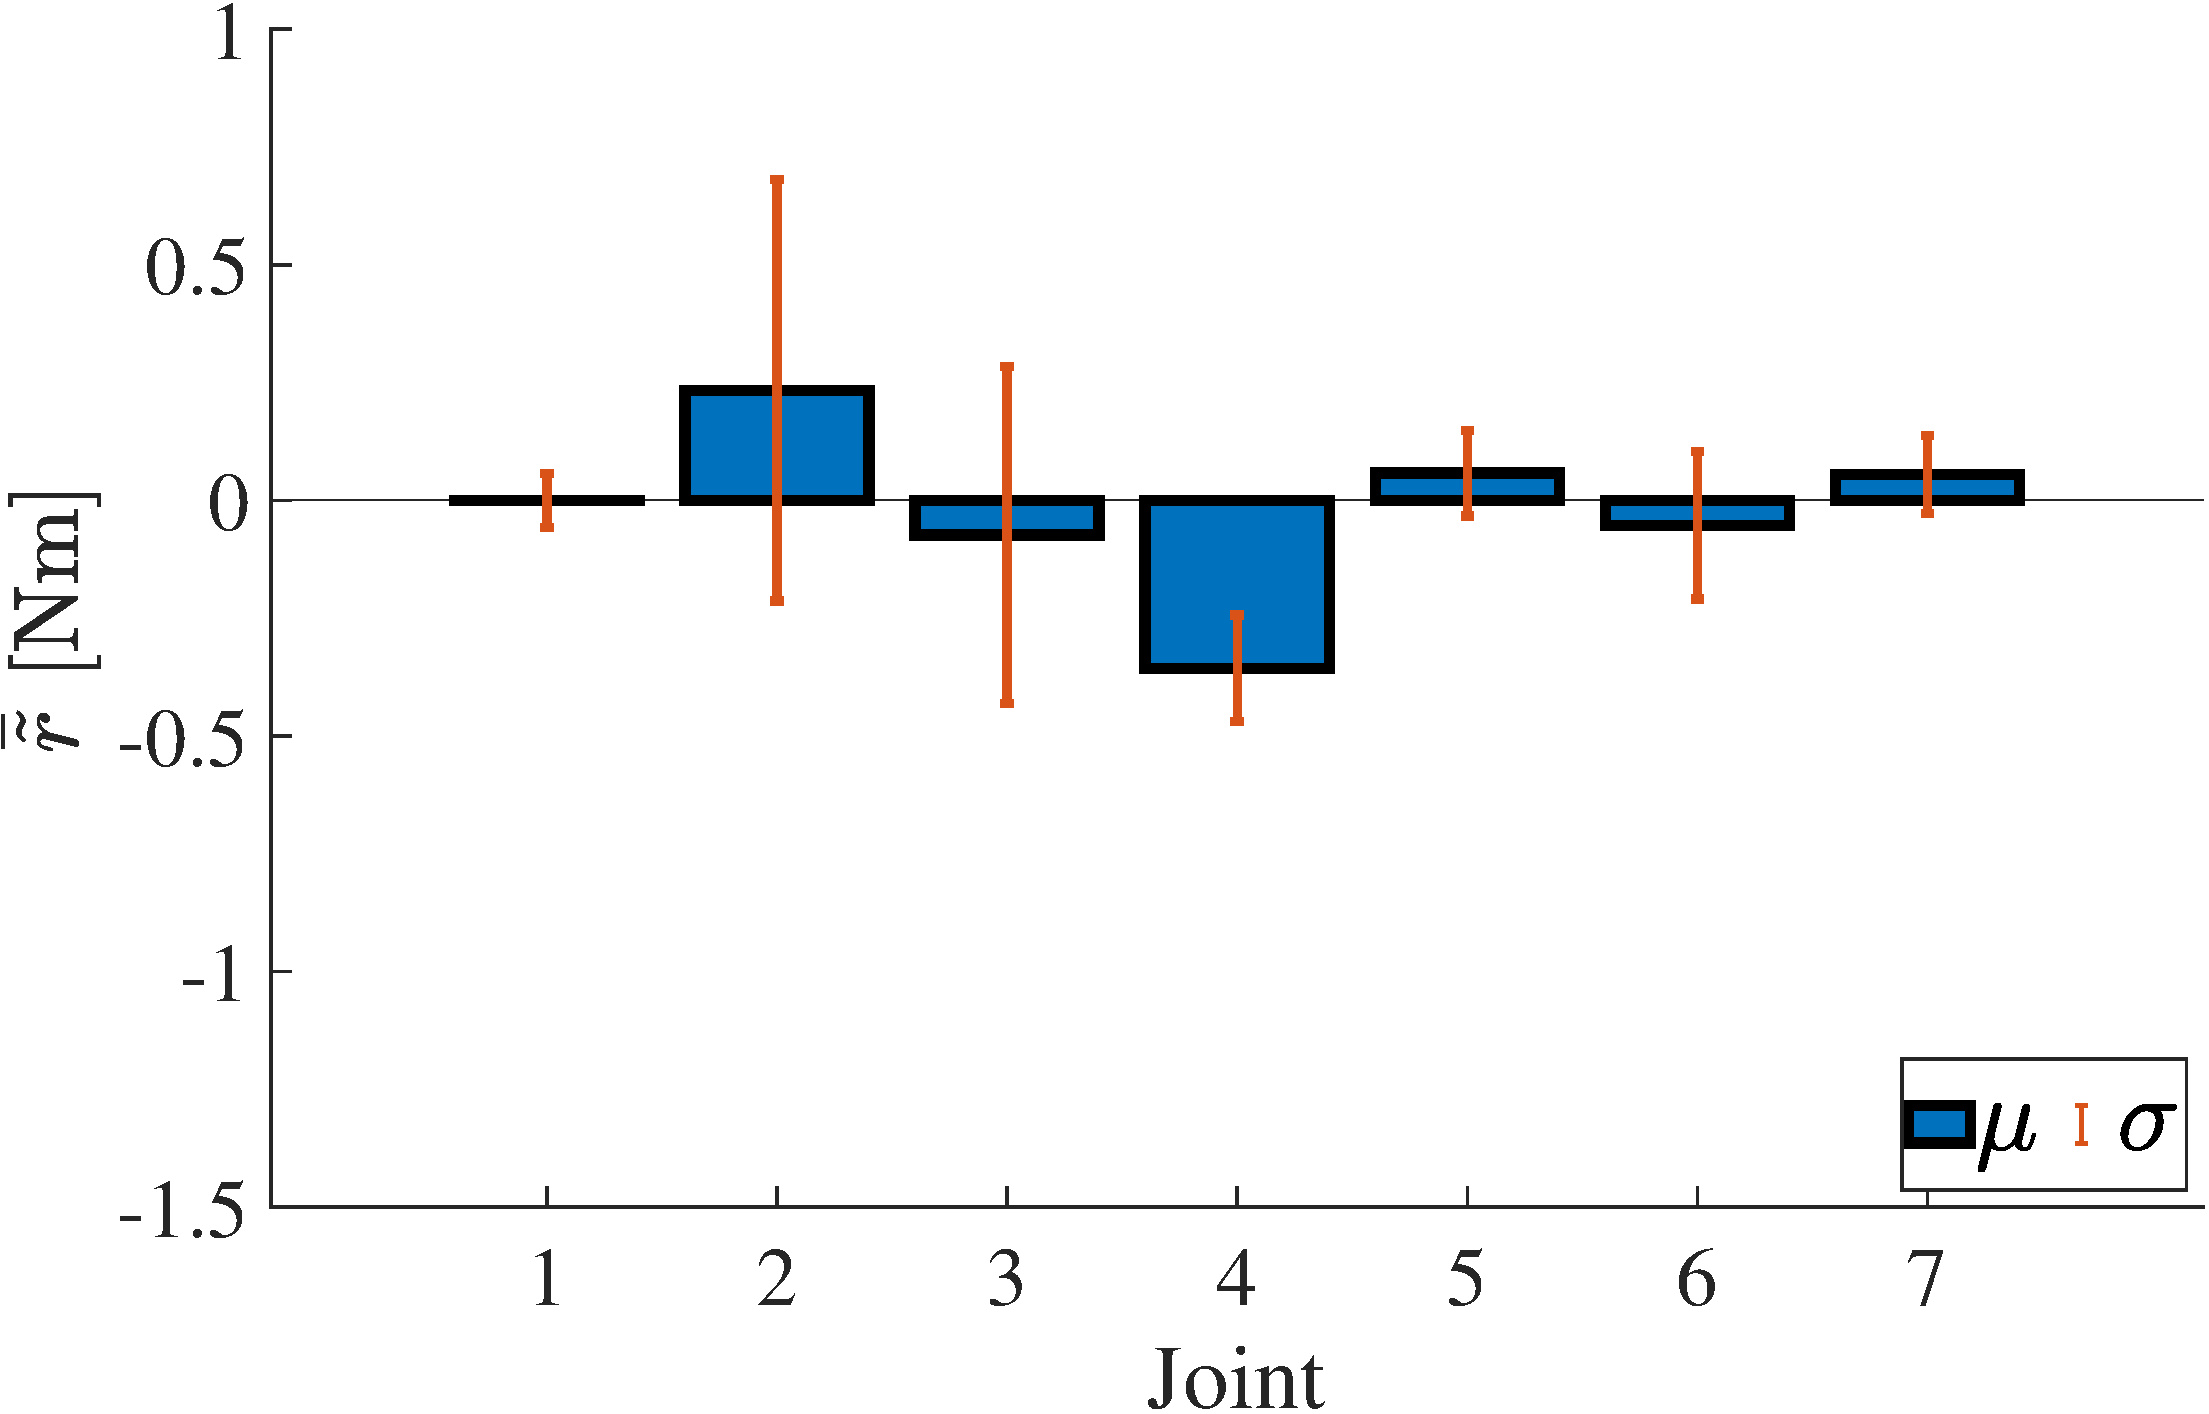
\includegraphics[width= 0.23\textwidth]{fig/residual_abs_error.pdf} \label{fig:residual_abs_error}}			
%\hspace*{\fill}
%\caption[] {\label{fig:panda_inverse_dynamics_torque_estimation} Experimental results: average absolute error for \subref{fig:panda_torque_error_sid_statistics} SID and \subref{fig:panda_torque_error_ril_statistics} RIL, \subref{fig:momentum_residual_average} momentum average residual and \subref{fig:residual_abs_error} average absolute residual per joint.}
%\end{figure*}
%%---
%A goal of characterizing the inertial properties of the robot's body schema is to use it as an inverse dynamics model. Consequently, we assess here the accuracy of the inverse dynamics torques $ \hat{\bm{\tau}} $ that result from $ \hat{\bm{\theta}} $. For a different 25 seconds trajectory we: record its joint torques $ \bm{\tau} $, compute the corresponding torque estimates, and obtain the estimation error $ \tilde{\bm{\tau}}_{RIL} = \bm{\tau} - \hat{\bm{\tau}}_{RIL} $. The mean $ \mu $ and standard deviation $ \sigma $ of its value for all joints during the experiment is shown in Fig.~\ref{fig:panda_torque_error_ril_statistics}. Observe that estimation for the large torques in proximal joints was rather good. In contrast, the error was more apparent in distal joints, where torques had smaller magnitudes. Nonetheless, the generated inverse dynamics torque closely reproduce the measured ones. Moreover, it could be further improved as the robot keeps collecting more diverse data samples during operation. Additionally, we computed the SID inverse dynamics torques (denoted here by $ \tilde{\bm{\tau}}_{SID} = \bm{\tau} - \bm{\tau}_{SID} $). Notoriously, the torques are practically the same and the errors can be attributed to minor non modeled effects and observed noise ($\pm$\SI{0.5}{\newton\meter} in the measured torque signal).
%
%% SUBSECTION ========================================================================================
%\subsection{A measure of model quality}
%The parameter estimates $ \hat{\bm{\theta}} $ can be used to reconstruct the standard rigid body dynamics model of the robot, i.e.
%\begin{equation}\label{eq:robt_dynamics_eq}
%\hat{M}(\bm{q};\hat{\bm{\theta}})\ddot{\bm{q}} + \hat{c}(\bm{q},\dot{\bm{q}};\hat{\bm{\theta}})+ \hat{g}(\bm{q};\hat{\bm{\theta}}) = \bm{\tau}_m + \bm{\tau}_{ext} - \bm{\tau}_{\epsilon}
%\end{equation}
%with $ \hat{M} $ being the robot mass matrix, $ \hat{\bm{c}} $ is the vector of centrifugal and Coriolis forces and $ \hat{\bm{g}} $ is the gravity torque vector. The RHS of \eqref{eq:robt_dynamics_eq} includes the motor, external and modeling error torques, respectively. 
%
%To provide further insight into the quality of a given set of learned inertial parameters, we used a momentum observer \cite{Haddadin2017Robotcollisionssurvey} whose output is given by:
%%---
%\begin{align}
%\bm{r}(t) &= \bm{K}\left(\bm{p}(t) - \int_{0}^{t}\left(\bm{\tau}_m - \hat{\bm{g}} - \hat{c}  \dot{\hat{\bm{M}}}+ \bm{r} \right)ds - \bm{p}(0)\right)\label{eq:observer_residual}
%\end{align}
%%---
%where $ \bm{p}=\hat{\bm{M}}(\bm{q})\dot{\bm{q}} $ is the generalized momentum estimate, $ \bm{K} $ is a diagonal matrix of positive values and $ \bm{r} $ is the monitoring residual. As the observer depends on an estimated model, then $ \bm{r} $ would converge to zero only if a perfect model is available and if no external torque is acting on the robot (i.e. $ \bm{\tau}_{ext}=0 $). Assuming the latter, then, by differentiating \eqref{eq:observer_residual} we obtain the residual dynamics $ \dot{\bm{r}}=-\bm{K}\left(\bm{\tau}_\epsilon + \bm{r}\right) $, whose solution converges asymptotically to $ \bm{\tau}_\epsilon $. We ran the momentum observer on the test trajectory and used two models: (a) one from $ \hat{\bm{\theta}}_{SID} $ and (b) $ \hat{\bm{\theta}}_{RIL} $. Fig.~\ref{fig:momentum_residual_average} shows the average of the residuals $ \bar{\bm{r}} $ for all seven joints for SID and RIL, where clearly $ \bar{\bm{r}}_{SID} \approx \bar{\bm{r}}_{RIL} $ . In Fig.~\ref{fig:residual_abs_error} we show the mean and standard deviation for the difference of the residuals of each joint $ \tilde{r}_i $; where it is apparent that the differences are negligible.
%
%% SUBSECTION ========================================================================================
%\subsection{Discussion}\label{sec:discussion}
%RIL comes with a few challenges. First, parameter convergence is slower than conventional euclidean unconstrained methods. Second, due to manifold operators, generating Riemannian updates is computationally more demanding. Third, RAMSGrad seems to be more sensitive to the learning rate $\alpha$ than its Euclidean homologue, which can be attributed to the curvature of $ \mathcal{M} $. Fourth, the algorithm's performance was hindered by measurement noise. Despite these challenges, RIL presents interesting areas of opportunity. For instance, although we used the standard values for the decay rates $ \beta_1 $ and $ \beta_2 $ further research can determine more appropriate values which can eventually cope with the learning rate challenge. Likewise a better use of the replay buffer $ \mathcal{B} $ and the mini batches $\mathcal{X}$ together with a more computationally efficient implementation can help leveraging past information to get a better parameter convergence and reduce the impact of noise. Furthermore, as discovering the body schema is in itself a self-driven task, developing a reward-based online motion strategy that induces efficient self exploration of the state space can contribute to a faster learning of the inertial parameters. A key point is that, unlike other algorithms, we do not need here any  previous knowledge to determine the initial guess, requiring only that $\hat{\bm{P}}_0 \in \mathcal{S}^4_{++}$. Additionally, the observed experimental inverse dynamics errors are comparable with those obtained by other offline methods using full data batches (e.g. see results in \cite{Sousa2019Inertiatensorproperties, Wensing2017Linearmatrixinequalities}) but with the added benefit of online learning. Moreover, from the relatively small values in the residual differences and inverse dynamics torques we can conclude that the model from RIL is qualitatively comparable to that from SID. Finally, there is the most appealing benefit: full physical feasibility at every time step. This guarantees valid incrementally-learned parameters that generate accurate inverse dynamics torques and can be used in other model-based techniques.
%
%% ===================================================================================================
%%                                                 |                                                 |
%%                                                 |                                                 |
%% -------------------------------------------- SECTION ---------------------------------------------|
%%                                                 |                                                 |
%%                                                 |                                                 |
%% ===================================================================================================
%\section{Conclusions}\label{sec:conclusion}
%We introduced the RIL method to characterize the dynamical properties of a robot's body schema. 
%Analysis on a virtual manipulator confirmed that RIL provides guarantees on the physical feasibility and learns consistent parameters at all times without prior information. Although experiments on a real robot exhibited high sensitivity to noise, the experience replay buffer helped to obtain parameter updates with reduced variability. Analysis of the inverse dynamics torques and modeling errors indicate that RIL is able to produce valid sets of inertial parameters that can generate accurate inverse dynamic torques and that result in consistent models. RIL opens pathways towards adaptable models that respect physical constraints, thus, positively impacting control and safety applications where failing to provide valid parameters may induce instabilities. Finally, we see potential in the method to be naturally complemented with a learning scheme that computes excitation motions online.


%\chapter{Introduction}\label{ch:introduction}
%In this final section the possible contribution of this thesis to future industrial applications as well as important new research directions are elaborated.

\section{Applications}
\input{chapter/outlook/applications}

\section{Further Research}
\input{chapter/outlook/research}
%\chapter{Theoretical Framework}\label{ch:foundations}
%In this final section the possible contribution of this thesis to future industrial applications as well as important new research directions are elaborated.

\section{Applications}
\input{chapter/outlook/applications}

\section{Further Research}
\input{chapter/outlook/research}
%\chapter{System Architecture and Validation Cases}\label{ch:architecture}
%In this final section the possible contribution of this thesis to future industrial applications as well as important new research directions are elaborated.

\section{Applications}
\input{chapter/outlook/applications}

\section{Further Research}
\input{chapter/outlook/research}
%\chapter{Experimental Analysis}\label{ch:experiments}
%In this final section the possible contribution of this thesis to future industrial applications as well as important new research directions are elaborated.

\section{Applications}
\input{chapter/outlook/applications}

\section{Further Research}
\input{chapter/outlook/research}


%\chapter{Introduction}\label{ch:introduction}
%In this final section the possible contribution of this thesis to future industrial applications as well as important new research directions are elaborated.

\section{Applications}
\input{chapter/outlook/applications}

\section{Further Research}
\input{chapter/outlook/research}
%\chapter{Related Work}
\section{Robot Platforms}
\section{Control}
\section{Skill Models}
\section{Taxonomies}
\section{Skill Learning}

\chapter{Taxonomy of Manipulation Skills}
\section{Introduction (taxonomy-introduction)}
\subsection{Definition of Tactile Skill (taxonomy-tactile skill)}
\subsection{Hypothesis (taxonomy-hypothesis)}
\section{Taxonomy}
\subsection{Process Definition (taxonomy-process definition)}
\subsection{Graph-guided Tactile Policies (taxonomy-ggtwrep)}
\subsection{Taxonomy (taxonomy-taxonomy)}
\subsection{Synthesis Procedure (taxonomy-synthesis)}
\section{Experiments}
\subsection{Setup (taxonomy-setup)}
\subsection{Results (taxonomy-results)}
\section{Discussion (taxonomy-discussion)}

\chapter{Manipulation Skill Learning}
\section{Introduction (transfer-introduction, comparison-introduction)}
\section{Methods}
\subsection{Algorithms (framework-algorithms, dl-algorithms}
\subsubsection{BO}
\subsubsection{CMA-ES}
\subsubsection{PSP}
\subsection{Metrics (transfer-metrics)}
\subsubsection{Cost function etc.}
\subsubsection{Transfer Metrics}
\subsection{Knowledge transfer (transfer-knowledge)}
\section{First Experiments (framework)}
\subsection{Setup}
\subsection{Results}
\subsection{Discussion/Conclusion}
\section{Comparison to DL (dl)}
\subsection{Comparison Paper: Setup}
\subsection{Comparison Paper: Results}
\subsection{Comparison Paper: Discussion/Conclusion}
\section{Transfer Learning (transfer)}
\subsection{Transfer Learning Paper: Hypothesis}
\subsection{Transfer Learning Paper: Setup}
\subsection{Transfer Learning Paper: Results}
\subsection{Transfer Learning Paper: Discussion}
\section{Performance Evaluation (comparison)}
\subsection{Introduction}
\subsection{Setup}
\subsection{Results}
\subsection{Discussion/Conclusion}
%\chapter{Related Work}\label{ch:related}
%In this final section the possible contribution of this thesis to future industrial applications as well as important new research directions are elaborated.

\section{Applications}
\input{chapter/outlook/applications}

\section{Further Research}
\input{chapter/outlook/research}
% \chapter{Application Cases}\label{ch:applications}
% In this final section the possible contribution of this thesis to future industrial applications as well as important new research directions are elaborated.

\section{Applications}
\input{chapter/outlook/applications}

\section{Further Research}
\input{chapter/outlook/research}
% \chapter{Taxonomy-Based Manipulation Skill Modeling}\label{ch:taxonomy}
% In this final section the possible contribution of this thesis to future industrial applications as well as important new research directions are elaborated.

\section{Applications}
\input{chapter/outlook/applications}

\section{Further Research}
\input{chapter/outlook/research}
% \chapter{Manipulation Skill Learning}\label{ch:learning}
% In this final section the possible contribution of this thesis to future industrial applications as well as important new research directions are elaborated.

\section{Applications}
\input{chapter/outlook/applications}

\section{Further Research}
\input{chapter/outlook/research}
% \chapter{Software}\label{ch:software}
% In this final section the possible contribution of this thesis to future industrial applications as well as important new research directions are elaborated.

\section{Applications}
\input{chapter/outlook/applications}

\section{Further Research}
\input{chapter/outlook/research}
%\chapter{Conclusion}\label{ch:conclusion}
%In this final section the possible contribution of this thesis to future industrial applications as well as important new research directions are elaborated.

\section{Applications}
\input{chapter/outlook/applications}

\section{Further Research}
\input{chapter/outlook/research}

%%%%%%%%%%%%%%%%%%%%%%%%%%%%%%%%%%%%%%%%%%%%%%%%%%%%%%%%%%%%%%%%
% appendix
%%%%%%%%%%%%%%%%%%%%%%%%%%%%%%%%%%%%%%%%%%%%%%%%%%%%%%%%%%%%%%%%
%\begin{appendix}
%\addcontentsline{toc}{chapter}{Appendix}
%In this final section the possible contribution of this thesis to future industrial applications as well as important new research directions are elaborated.

\section{Applications}
\input{chapter/outlook/applications}

\section{Further Research}
\input{chapter/outlook/research}
%\end{appendix}



%\cleardoublepage\currentpdfbookmark{List of Figures}{phd_listoffigures}
%\listoffigures
%
%\cleardoublepage\currentpdfbookmark{List of Tables}{phd_listoftables}
%\listoftables

%%%%%%%%%%%%%%%%%%%%%%%%%%%%%%%%%%%%%%%%%%%%%%%%%%%%%%%%%%%%%%%%
% bibliography
%%%%%%%%%%%%%%%%%%%%%%%%%%%%%%%%%%%%%%%%%%%%%%%%%%%%%%%%%%%%%%%%
%\cleardoublepage
\ifpdf
	\phantomsection 
\fi
\addcontentsline{toc}{chapter}{\bibname}

%\bibliographystyle{alpha}
\bibliographystyle{./IEEEtran}
\bibliography{bibliography/dissertation_bibliography}
%\printbibliography
%%%%%%%%%%%%%%%%%%%%%%%%%%%%%%%%%%%%%%%%%%%%%%%%%%%%%%%%%%%%%%%%
%%%%%%%%%%%%%%%%%%%%%%%%%%%%%%%%%%%%%%%%%%%%%%%%%%%%%%%%%%%%%%%%
%%%%%%%%%%%%%%%%%%%%%%%%%%%%%%%%%%%%%%%%%%%%%%%%%%%%%%%%%%%%%%%%
\end{document}

%%%%%%%%%%%%%%%%%%%%%%%%%%%%%%%%%%%%%%%%%%%%%%%%%%%%%%%%%%%%%%%%
